\documentclass[]{book}
\usepackage{lmodern}
\usepackage{amssymb,amsmath}
\usepackage{ifxetex,ifluatex}
\usepackage{fixltx2e} % provides \textsubscript
\ifnum 0\ifxetex 1\fi\ifluatex 1\fi=0 % if pdftex
  \usepackage[T1]{fontenc}
  \usepackage[utf8]{inputenc}
\else % if luatex or xelatex
  \ifxetex
    \usepackage{mathspec}
  \else
    \usepackage{fontspec}
  \fi
  \defaultfontfeatures{Ligatures=TeX,Scale=MatchLowercase}
\fi
% use upquote if available, for straight quotes in verbatim environments
\IfFileExists{upquote.sty}{\usepackage{upquote}}{}
% use microtype if available
\IfFileExists{microtype.sty}{%
\usepackage{microtype}
\UseMicrotypeSet[protrusion]{basicmath} % disable protrusion for tt fonts
}{}
\usepackage[margin=1in]{geometry}
\usepackage{hyperref}
\hypersetup{unicode=true,
            pdftitle={Data 624 - HA Assignments (HW1)},
            pdfauthor={Group 1: Andrew Carson, Nathan Cooper, Baron Curtin, Heather Geiger},
            pdfborder={0 0 0},
            breaklinks=true}
\urlstyle{same}  % don't use monospace font for urls
\usepackage{color}
\usepackage{fancyvrb}
\newcommand{\VerbBar}{|}
\newcommand{\VERB}{\Verb[commandchars=\\\{\}]}
\DefineVerbatimEnvironment{Highlighting}{Verbatim}{commandchars=\\\{\}}
% Add ',fontsize=\small' for more characters per line
\usepackage{framed}
\definecolor{shadecolor}{RGB}{248,248,248}
\newenvironment{Shaded}{\begin{snugshade}}{\end{snugshade}}
\newcommand{\AlertTok}[1]{\textcolor[rgb]{0.94,0.16,0.16}{#1}}
\newcommand{\AnnotationTok}[1]{\textcolor[rgb]{0.56,0.35,0.01}{\textbf{\textit{#1}}}}
\newcommand{\AttributeTok}[1]{\textcolor[rgb]{0.77,0.63,0.00}{#1}}
\newcommand{\BaseNTok}[1]{\textcolor[rgb]{0.00,0.00,0.81}{#1}}
\newcommand{\BuiltInTok}[1]{#1}
\newcommand{\CharTok}[1]{\textcolor[rgb]{0.31,0.60,0.02}{#1}}
\newcommand{\CommentTok}[1]{\textcolor[rgb]{0.56,0.35,0.01}{\textit{#1}}}
\newcommand{\CommentVarTok}[1]{\textcolor[rgb]{0.56,0.35,0.01}{\textbf{\textit{#1}}}}
\newcommand{\ConstantTok}[1]{\textcolor[rgb]{0.00,0.00,0.00}{#1}}
\newcommand{\ControlFlowTok}[1]{\textcolor[rgb]{0.13,0.29,0.53}{\textbf{#1}}}
\newcommand{\DataTypeTok}[1]{\textcolor[rgb]{0.13,0.29,0.53}{#1}}
\newcommand{\DecValTok}[1]{\textcolor[rgb]{0.00,0.00,0.81}{#1}}
\newcommand{\DocumentationTok}[1]{\textcolor[rgb]{0.56,0.35,0.01}{\textbf{\textit{#1}}}}
\newcommand{\ErrorTok}[1]{\textcolor[rgb]{0.64,0.00,0.00}{\textbf{#1}}}
\newcommand{\ExtensionTok}[1]{#1}
\newcommand{\FloatTok}[1]{\textcolor[rgb]{0.00,0.00,0.81}{#1}}
\newcommand{\FunctionTok}[1]{\textcolor[rgb]{0.00,0.00,0.00}{#1}}
\newcommand{\ImportTok}[1]{#1}
\newcommand{\InformationTok}[1]{\textcolor[rgb]{0.56,0.35,0.01}{\textbf{\textit{#1}}}}
\newcommand{\KeywordTok}[1]{\textcolor[rgb]{0.13,0.29,0.53}{\textbf{#1}}}
\newcommand{\NormalTok}[1]{#1}
\newcommand{\OperatorTok}[1]{\textcolor[rgb]{0.81,0.36,0.00}{\textbf{#1}}}
\newcommand{\OtherTok}[1]{\textcolor[rgb]{0.56,0.35,0.01}{#1}}
\newcommand{\PreprocessorTok}[1]{\textcolor[rgb]{0.56,0.35,0.01}{\textit{#1}}}
\newcommand{\RegionMarkerTok}[1]{#1}
\newcommand{\SpecialCharTok}[1]{\textcolor[rgb]{0.00,0.00,0.00}{#1}}
\newcommand{\SpecialStringTok}[1]{\textcolor[rgb]{0.31,0.60,0.02}{#1}}
\newcommand{\StringTok}[1]{\textcolor[rgb]{0.31,0.60,0.02}{#1}}
\newcommand{\VariableTok}[1]{\textcolor[rgb]{0.00,0.00,0.00}{#1}}
\newcommand{\VerbatimStringTok}[1]{\textcolor[rgb]{0.31,0.60,0.02}{#1}}
\newcommand{\WarningTok}[1]{\textcolor[rgb]{0.56,0.35,0.01}{\textbf{\textit{#1}}}}
\usepackage{longtable,booktabs}
\usepackage{graphicx,grffile}
\makeatletter
\def\maxwidth{\ifdim\Gin@nat@width>\linewidth\linewidth\else\Gin@nat@width\fi}
\def\maxheight{\ifdim\Gin@nat@height>\textheight\textheight\else\Gin@nat@height\fi}
\makeatother
% Scale images if necessary, so that they will not overflow the page
% margins by default, and it is still possible to overwrite the defaults
% using explicit options in \includegraphics[width, height, ...]{}
\setkeys{Gin}{width=\maxwidth,height=\maxheight,keepaspectratio}
\IfFileExists{parskip.sty}{%
\usepackage{parskip}
}{% else
\setlength{\parindent}{0pt}
\setlength{\parskip}{6pt plus 2pt minus 1pt}
}
\setlength{\emergencystretch}{3em}  % prevent overfull lines
\providecommand{\tightlist}{%
  \setlength{\itemsep}{0pt}\setlength{\parskip}{0pt}}
\setcounter{secnumdepth}{5}
% Redefines (sub)paragraphs to behave more like sections
\ifx\paragraph\undefined\else
\let\oldparagraph\paragraph
\renewcommand{\paragraph}[1]{\oldparagraph{#1}\mbox{}}
\fi
\ifx\subparagraph\undefined\else
\let\oldsubparagraph\subparagraph
\renewcommand{\subparagraph}[1]{\oldsubparagraph{#1}\mbox{}}
\fi

%%% Use protect on footnotes to avoid problems with footnotes in titles
\let\rmarkdownfootnote\footnote%
\def\footnote{\protect\rmarkdownfootnote}

%%% Change title format to be more compact
\usepackage{titling}

% Create subtitle command for use in maketitle
\newcommand{\subtitle}[1]{
  \posttitle{
    \begin{center}\large#1\end{center}
    }
}

\setlength{\droptitle}{-2em}

  \title{Data 624 - HA Assignments (HW1)}
    \pretitle{\vspace{\droptitle}\centering\huge}
  \posttitle{\par}
    \author{Group 1: Andrew Carson, Nathan Cooper, Baron Curtin, Heather Geiger}
    \preauthor{\centering\large\emph}
  \postauthor{\par}
      \predate{\centering\large\emph}
  \postdate{\par}
    \date{2019-03-02}

\usepackage{booktabs}
\usepackage{longtable}
\usepackage{array}
\usepackage{multirow}
\usepackage{wrapfig}
\usepackage{float}
\usepackage{colortbl}
\usepackage{pdflscape}
\usepackage{tabu}
\usepackage{threeparttable}
\usepackage{threeparttablex}
\usepackage[normalem]{ulem}
\usepackage{makecell}
\usepackage{xcolor}

\begin{document}
\maketitle

{
\setcounter{tocdepth}{1}
\tableofcontents
}
\hypertarget{introduction}{%
\chapter{Introduction}\label{introduction}}

The work herein constitutes the work of Andrew Carson, Nathan Cooper, Baron Curtin, and Heather Geiger in the course Data 624 towards completion of the first set of homework assignments due for Professor Burk.

\hypertarget{hw1}{%
\chapter{HW1}\label{hw1}}

\hypertarget{section}{%
\section{2.3}\label{section}}

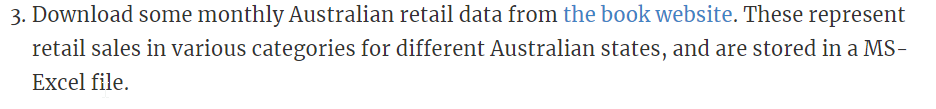
\includegraphics{./week1/2.3.png}

\hypertarget{a}{%
\subsection{a}\label{a}}

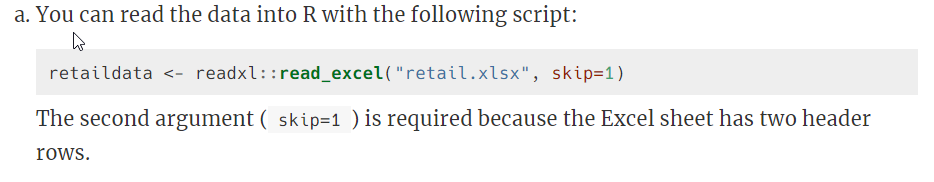
\includegraphics{./week1/2.3a.png}

\begin{Shaded}
\begin{Highlighting}[]
\NormalTok{retailData <-}\StringTok{  }\NormalTok{readxl}\OperatorTok{::}\KeywordTok{read_excel}\NormalTok{(}\StringTok{'./week1/retail.xlsx'}\NormalTok{, }\DataTypeTok{skip=}\DecValTok{1}\NormalTok{)}
\end{Highlighting}
\end{Shaded}

\hypertarget{b}{%
\subsection{b}\label{b}}

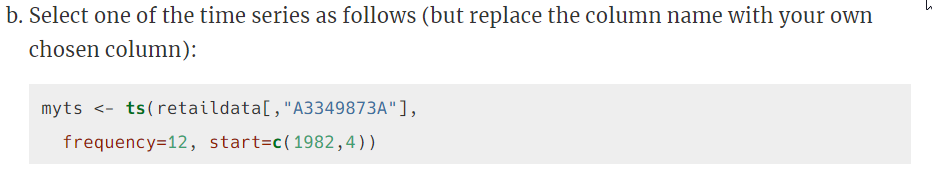
\includegraphics{./week1/2.3b.png}

\begin{Shaded}
\begin{Highlighting}[]
\NormalTok{myts <-}\StringTok{ }\KeywordTok{ts}\NormalTok{(retailData[, }\StringTok{"A3349338X"}\NormalTok{],}
           \DataTypeTok{frequency =} \DecValTok{12}\NormalTok{,}
           \DataTypeTok{start=}\KeywordTok{c}\NormalTok{(}\DecValTok{1982}\NormalTok{,}\DecValTok{4}\NormalTok{))}
\end{Highlighting}
\end{Shaded}

\hypertarget{c}{%
\subsection{c}\label{c}}

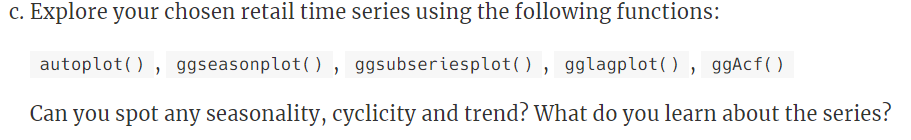
\includegraphics{./week1/2.3c.png}

\begin{Shaded}
\begin{Highlighting}[]
\KeywordTok{autoplot}\NormalTok{(myts[, }\StringTok{"A3349338X"}\NormalTok{]) }\OperatorTok{+}
\StringTok{  }\KeywordTok{ggtitle}\NormalTok{(}\StringTok{"Time Series Plot A3349338X"}\NormalTok{) }\OperatorTok{+}
\StringTok{  }\KeywordTok{xlab}\NormalTok{(}\StringTok{"Year"}\NormalTok{) }\OperatorTok{+}
\StringTok{  }\KeywordTok{ylab}\NormalTok{(}\StringTok{"Value"}\NormalTok{)}
\end{Highlighting}
\end{Shaded}

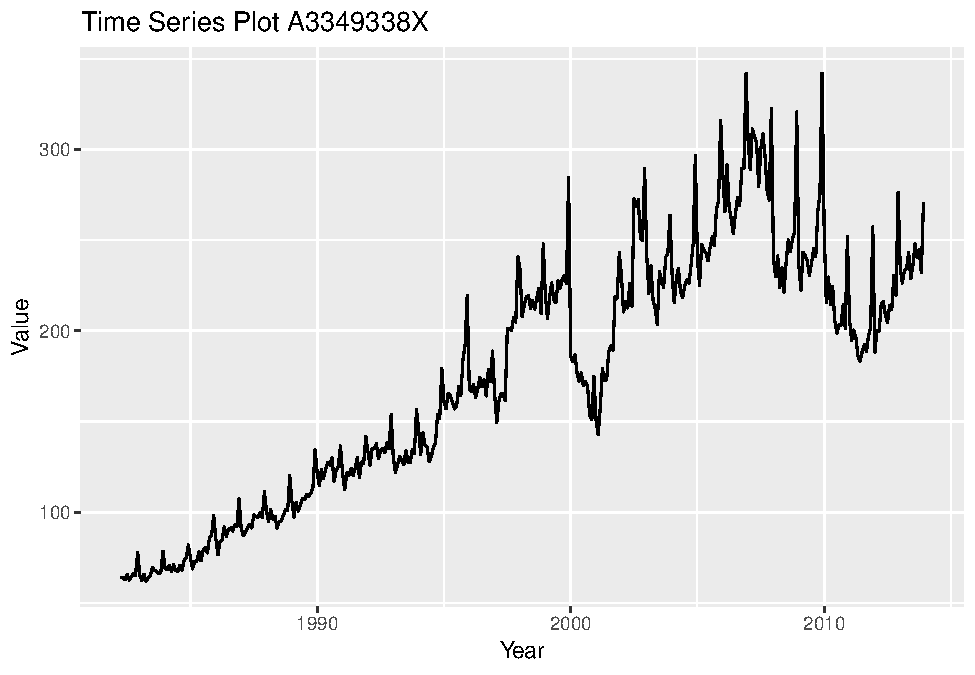
\includegraphics{_main_files/figure-latex/unnamed-chunk-5-1.pdf}

From the time series plot, we able to deduce:
* Trend: there is a clear upward trend over the duration of the time series

\begin{Shaded}
\begin{Highlighting}[]
\KeywordTok{ggseasonplot}\NormalTok{(myts, }\DataTypeTok{year.labels =}\NormalTok{ T) }\OperatorTok{+}
\StringTok{  }\KeywordTok{ggtitle}\NormalTok{(}\StringTok{"Seasonal plot: A3349338X"}\NormalTok{)}
\end{Highlighting}
\end{Shaded}

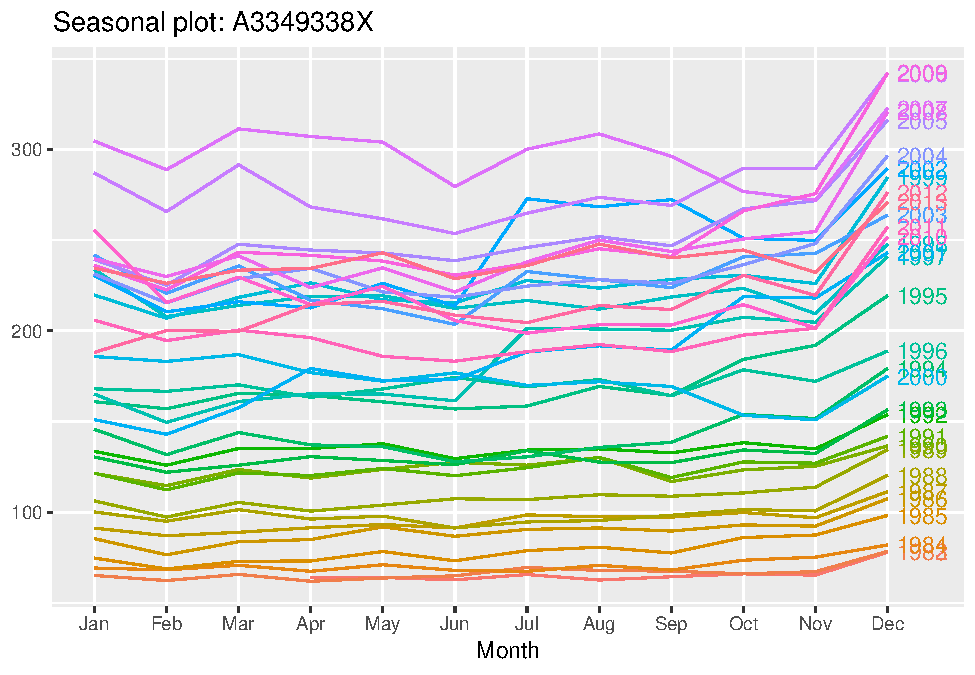
\includegraphics{_main_files/figure-latex/unnamed-chunk-6-1.pdf}

\begin{Shaded}
\begin{Highlighting}[]
\KeywordTok{ggsubseriesplot}\NormalTok{(myts) }\OperatorTok{+}
\StringTok{  }\KeywordTok{ggtitle}\NormalTok{(}\StringTok{"Seasonal subseries pllot: A3349338X"}\NormalTok{)}
\end{Highlighting}
\end{Shaded}

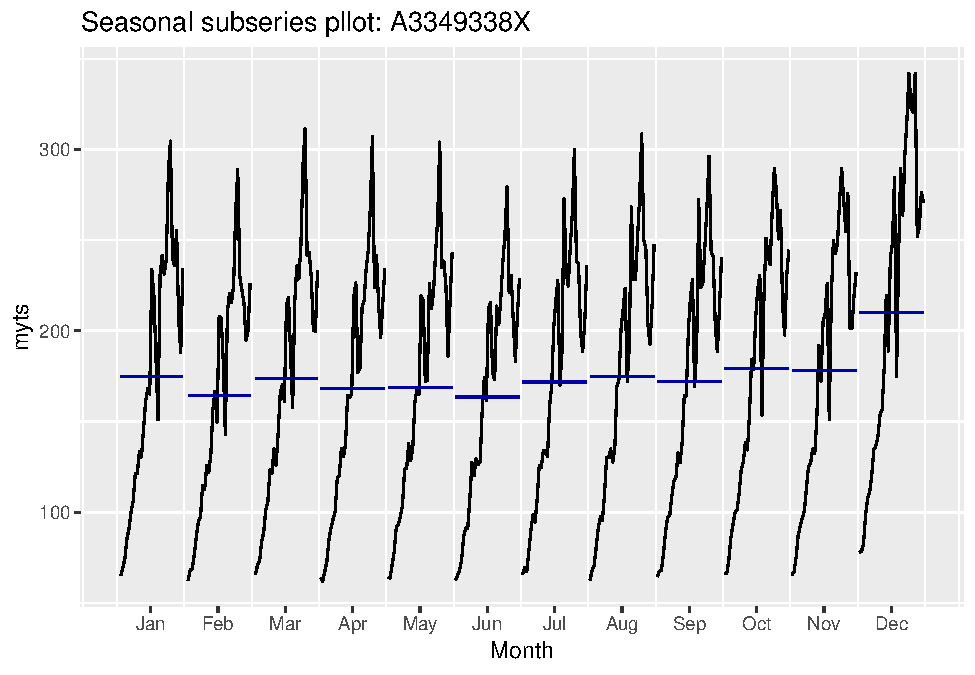
\includegraphics{_main_files/figure-latex/unnamed-chunk-6-2.pdf}

From the seasonal plot, we are able to deduce:
* Seasonality: there is some clear seasonality that exists among different month, however it is not without minor variation/deviation between the years
* December shows a clear uptick while February shows a clear downtick

\begin{Shaded}
\begin{Highlighting}[]
\KeywordTok{ggAcf}\NormalTok{(myts)}
\end{Highlighting}
\end{Shaded}

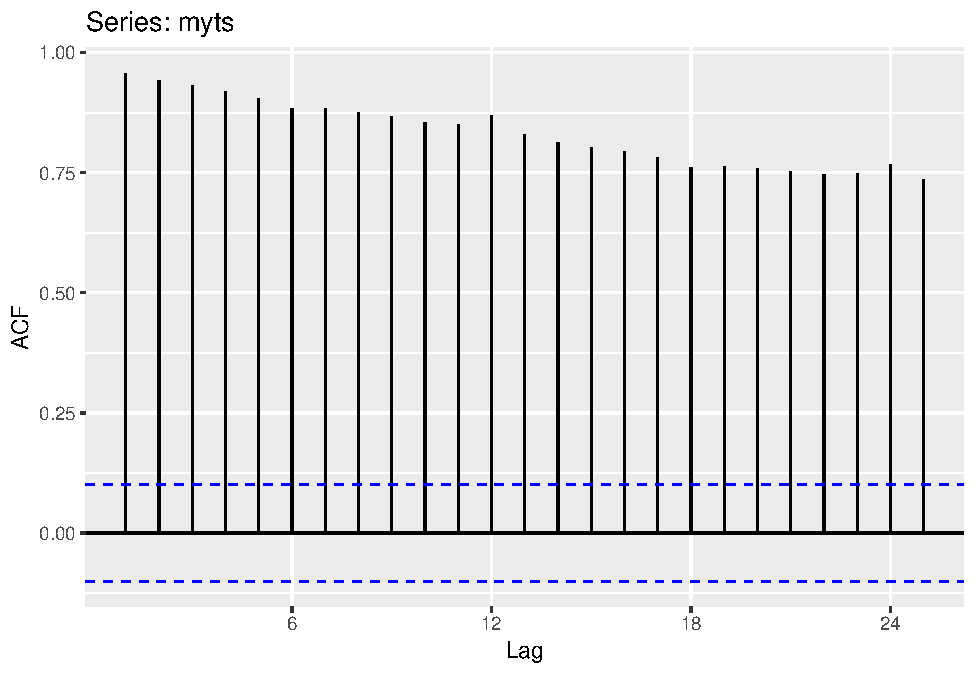
\includegraphics{_main_files/figure-latex/unnamed-chunk-7-1.pdf}

From the Acf plot, we are able to confirm:
* Trend: the autocorrelations are slowly decreasing as the lags are increasing

Conclusion:
* Trend exists in this time series and is slowly going upwrd
* Seasonality appears to exist however there are years that defy seasonality patterns
* There does not appear to be any cyclic behavior

\hypertarget{section-1}{%
\section{2.7}\label{section-1}}

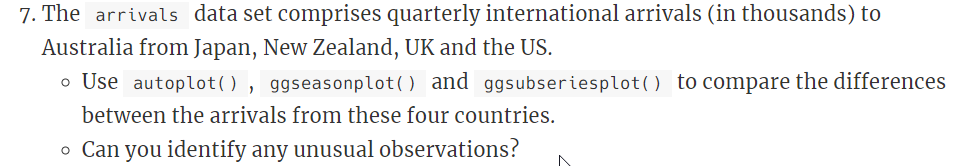
\includegraphics{./week1/2.7.png}

\begin{Shaded}
\begin{Highlighting}[]
\CommentTok{#arrivals <- data("arrivals")}
\end{Highlighting}
\end{Shaded}

\begin{Shaded}
\begin{Highlighting}[]
\KeywordTok{autoplot}\NormalTok{(arrivals) }\OperatorTok{+}
\StringTok{  }\KeywordTok{ggtitle}\NormalTok{(}\StringTok{"Arrivals Time Series"}\NormalTok{) }\OperatorTok{+}
\StringTok{  }\KeywordTok{facet_wrap}\NormalTok{(}\OperatorTok{~}\NormalTok{series)}
\end{Highlighting}
\end{Shaded}

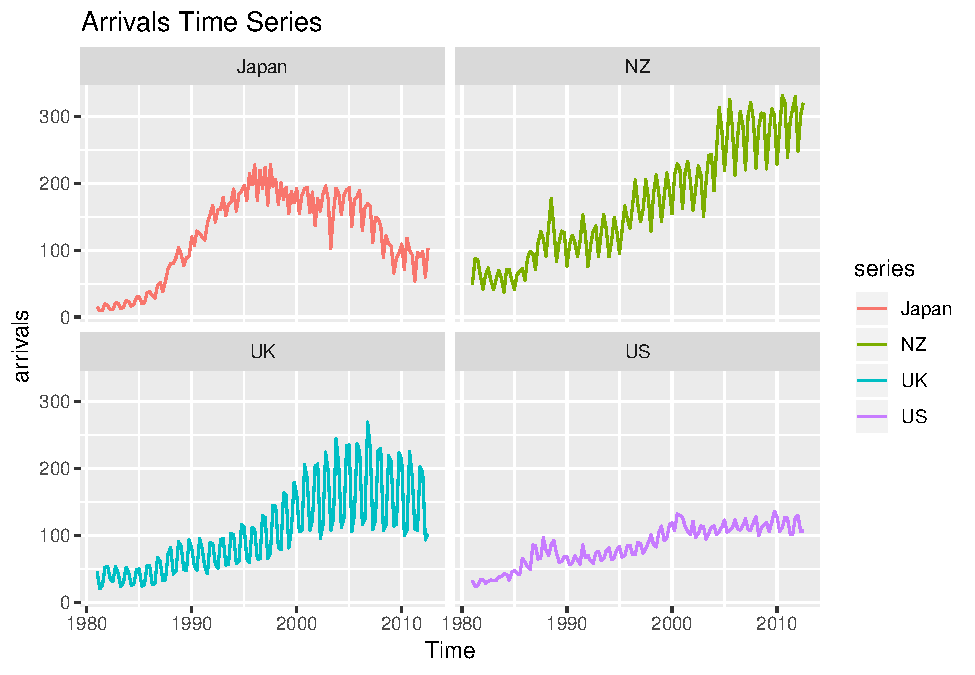
\includegraphics{_main_files/figure-latex/unnamed-chunk-9-1.pdf}

Observations:
* Japan seems to experience a an upward trend, reach an apex, and then experience a downward trend
* NZ, UK, and US all experience upward trends in arrivals albeit to different degrees
* UK appears to have the greatest variance in their arrival figures
* US has very little deviation in their arrival trend
* NZ has more fluctuation than US, but less than UK in their arrivals
* US on average has the lowest amount of arrivals

\begin{Shaded}
\begin{Highlighting}[]
\NormalTok{genSeasonPlot <-}\StringTok{ }\ControlFlowTok{function}\NormalTok{(country) \{}
  \KeywordTok{ggseasonplot}\NormalTok{(arrivals[, country]) }\OperatorTok{+}
\StringTok{    }\KeywordTok{ggtitle}\NormalTok{(}\KeywordTok{glue}\NormalTok{(}\StringTok{"Season Plot: \{country\}"}\NormalTok{))}
\NormalTok{\}}
\NormalTok{countries <-}\StringTok{ }\KeywordTok{c}\NormalTok{(}\StringTok{"Japan"}\NormalTok{, }\StringTok{"NZ"}\NormalTok{, }\StringTok{"US"}\NormalTok{, }\StringTok{"UK"}\NormalTok{)}
\NormalTok{countries }\OperatorTok
\StringTok{  }\KeywordTok{map}\NormalTok{(}\OperatorTok{~}\StringTok{ }\KeywordTok{genSeasonPlot}\NormalTok{(.x))}
\end{Highlighting}
\end{Shaded}

\begin{verbatim}
## [[1]]
\end{verbatim}

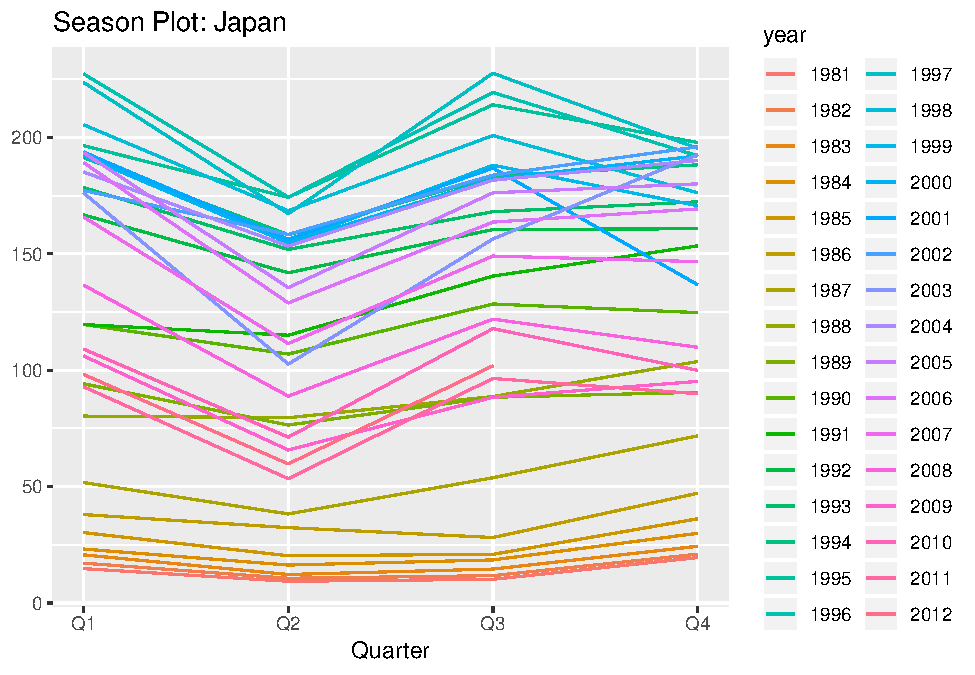
\includegraphics{_main_files/figure-latex/unnamed-chunk-10-1.pdf}

\begin{verbatim}
## 
## [[2]]
\end{verbatim}

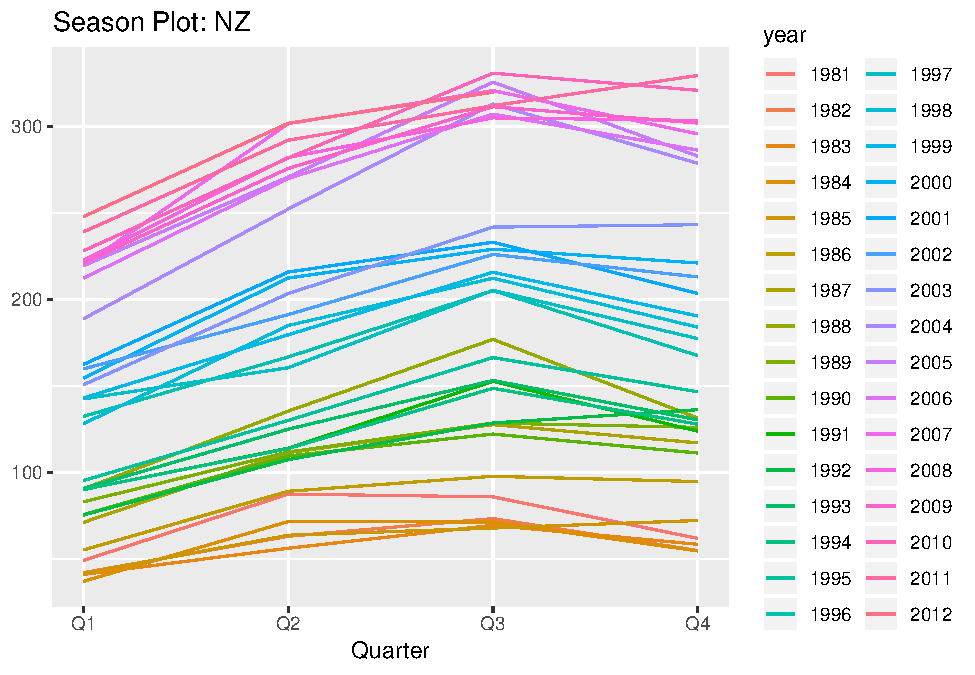
\includegraphics{_main_files/figure-latex/unnamed-chunk-10-2.pdf}

\begin{verbatim}
## 
## [[3]]
\end{verbatim}

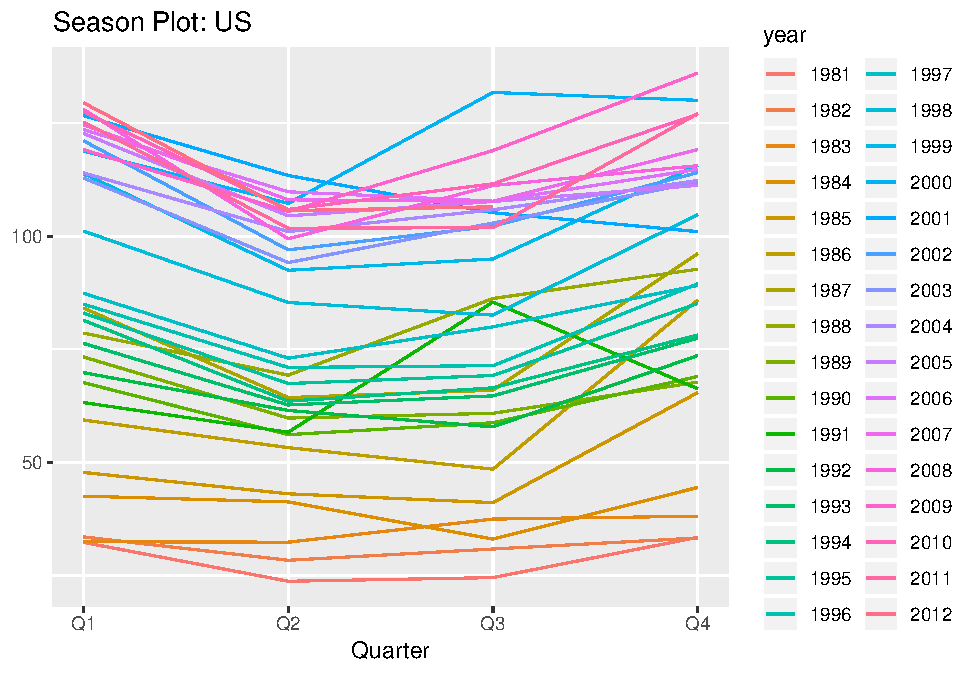
\includegraphics{_main_files/figure-latex/unnamed-chunk-10-3.pdf}

\begin{verbatim}
## 
## [[4]]
\end{verbatim}

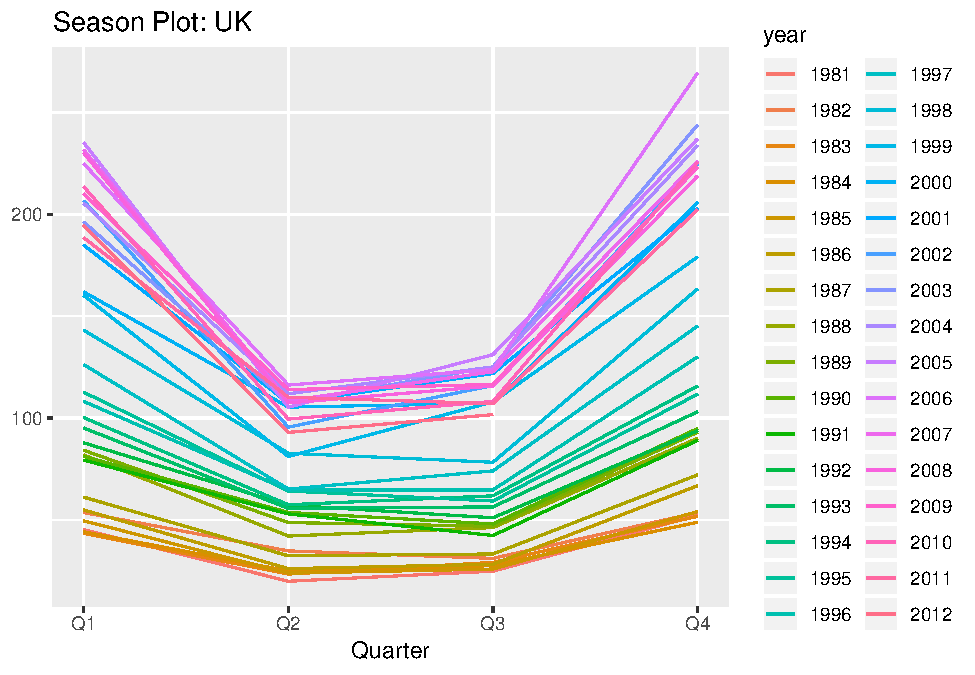
\includegraphics{_main_files/figure-latex/unnamed-chunk-10-4.pdf}

Observations from Seasonal Plots:
* Typically the countries will see their highest arrivals in Q3, however the UK appears to go against this seasonal pattern
* Q2 appears to be a down quarter for all countries except NZ
* Q1 is a low point for NZ, and generally a high point for the other countries

\begin{Shaded}
\begin{Highlighting}[]
\NormalTok{genSubSeasonPlot <-}\StringTok{ }\ControlFlowTok{function}\NormalTok{(country) \{}
  \KeywordTok{ggsubseriesplot}\NormalTok{(arrivals[, country]) }\OperatorTok{+}
\StringTok{    }\KeywordTok{ggtitle}\NormalTok{(}\KeywordTok{glue}\NormalTok{(}\StringTok{"Subseries Plot: \{country\}"}\NormalTok{))}
\NormalTok{\}}
\NormalTok{countries }\OperatorTok
\StringTok{  }\KeywordTok{map}\NormalTok{(}\OperatorTok{~}\StringTok{ }\KeywordTok{genSubSeasonPlot}\NormalTok{(.x))}
\end{Highlighting}
\end{Shaded}

\begin{verbatim}
## [[1]]
\end{verbatim}

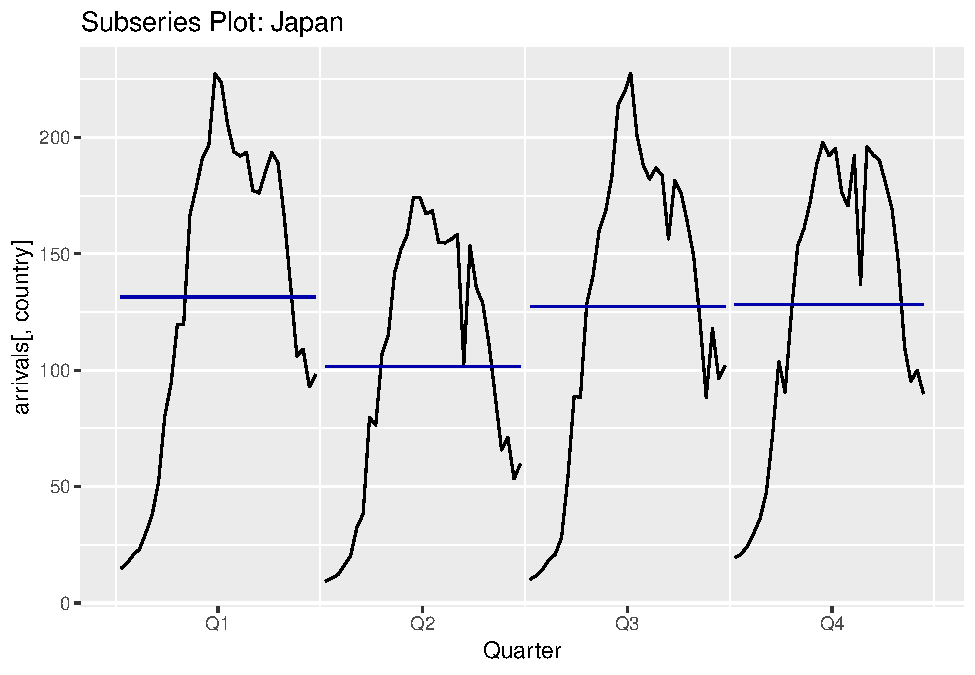
\includegraphics{_main_files/figure-latex/unnamed-chunk-11-1.pdf}

\begin{verbatim}
## 
## [[2]]
\end{verbatim}

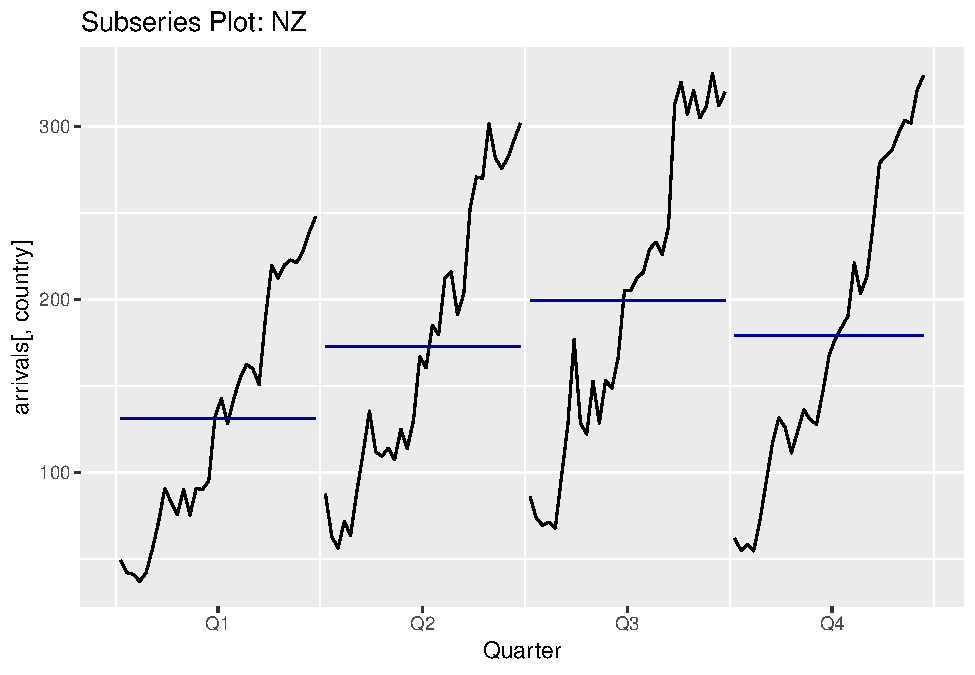
\includegraphics{_main_files/figure-latex/unnamed-chunk-11-2.pdf}

\begin{verbatim}
## 
## [[3]]
\end{verbatim}

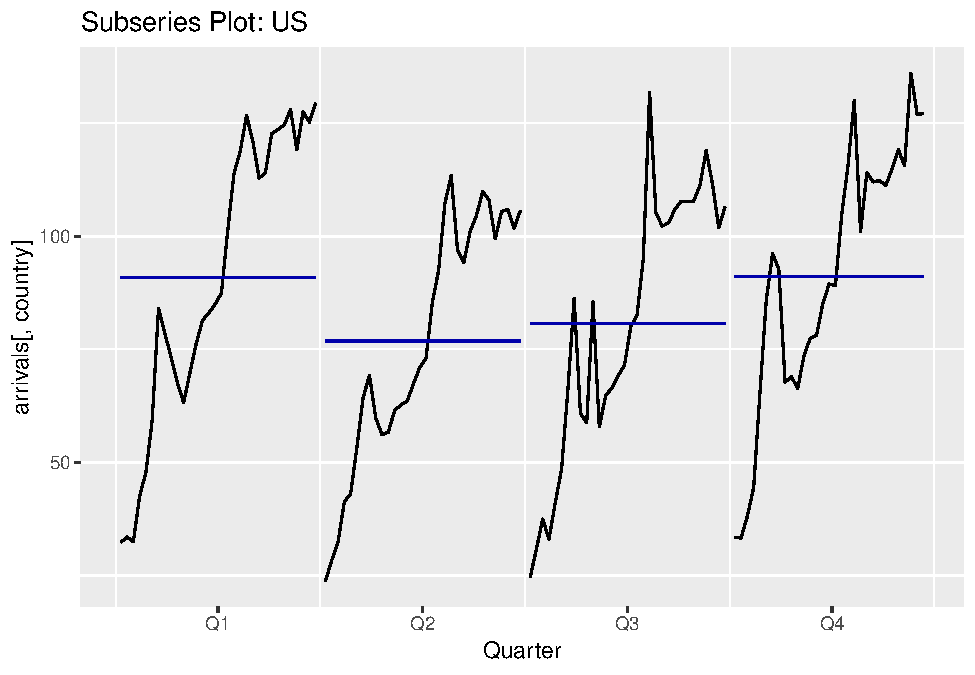
\includegraphics{_main_files/figure-latex/unnamed-chunk-11-3.pdf}

\begin{verbatim}
## 
## [[4]]
\end{verbatim}

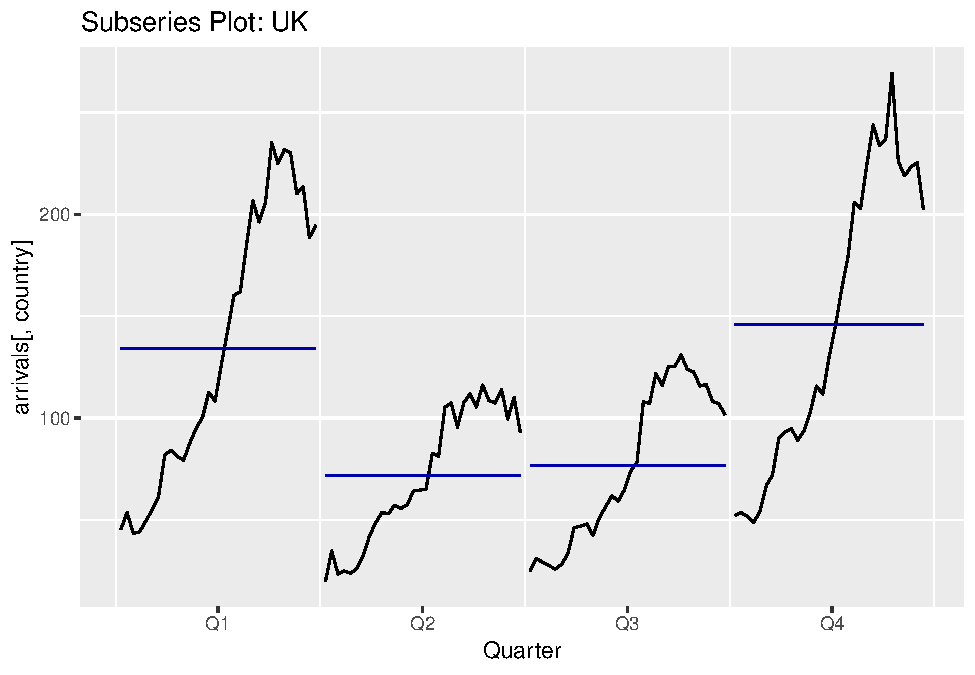
\includegraphics{_main_files/figure-latex/unnamed-chunk-11-4.pdf}

Observations:
* Japan's mean stays relatively flat across the quarters outside of Q2
* US also remains relatively consistent and further backs up the lack of deviation point made earlier
* UK experiences the most arrivals in Q1 and A4

\hypertarget{section-2}{%
\section{2.10}\label{section-2}}

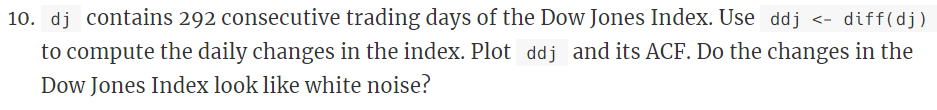
\includegraphics{./week1/2.10.png}

\begin{Shaded}
\begin{Highlighting}[]
\KeywordTok{data}\NormalTok{(}\StringTok{"dj"}\NormalTok{)}
\NormalTok{ddj <-}\StringTok{ }\KeywordTok{diff}\NormalTok{(dj)}
\end{Highlighting}
\end{Shaded}

\begin{Shaded}
\begin{Highlighting}[]
\KeywordTok{autoplot}\NormalTok{(ddj)}
\end{Highlighting}
\end{Shaded}

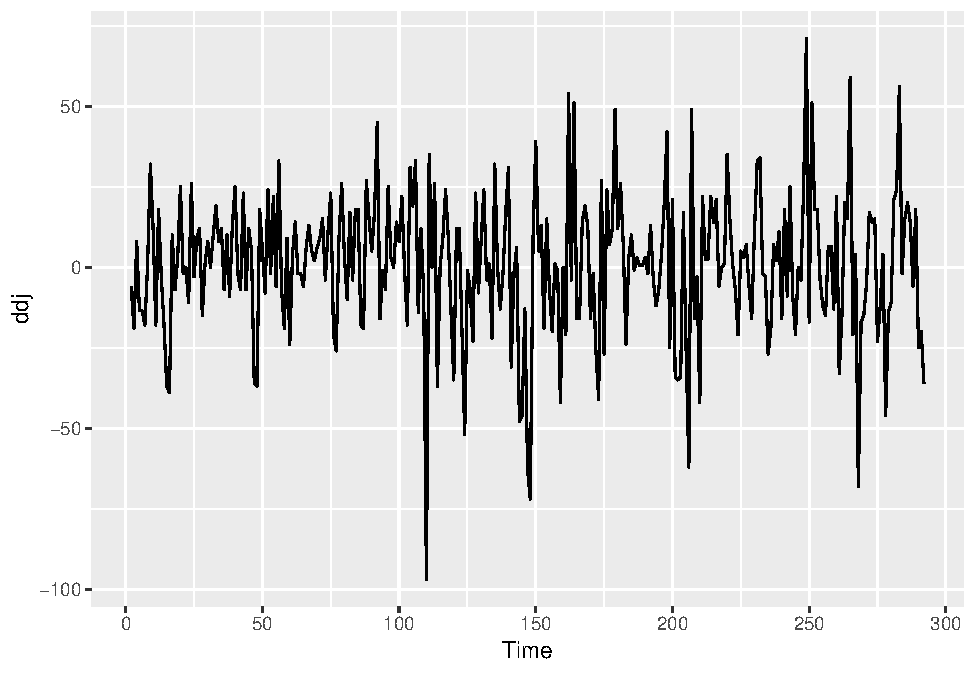
\includegraphics{_main_files/figure-latex/unnamed-chunk-13-1.pdf}

The autoplot appears to show random variation with peaks and valleys

\begin{Shaded}
\begin{Highlighting}[]
\KeywordTok{ggAcf}\NormalTok{(ddj)}
\end{Highlighting}
\end{Shaded}

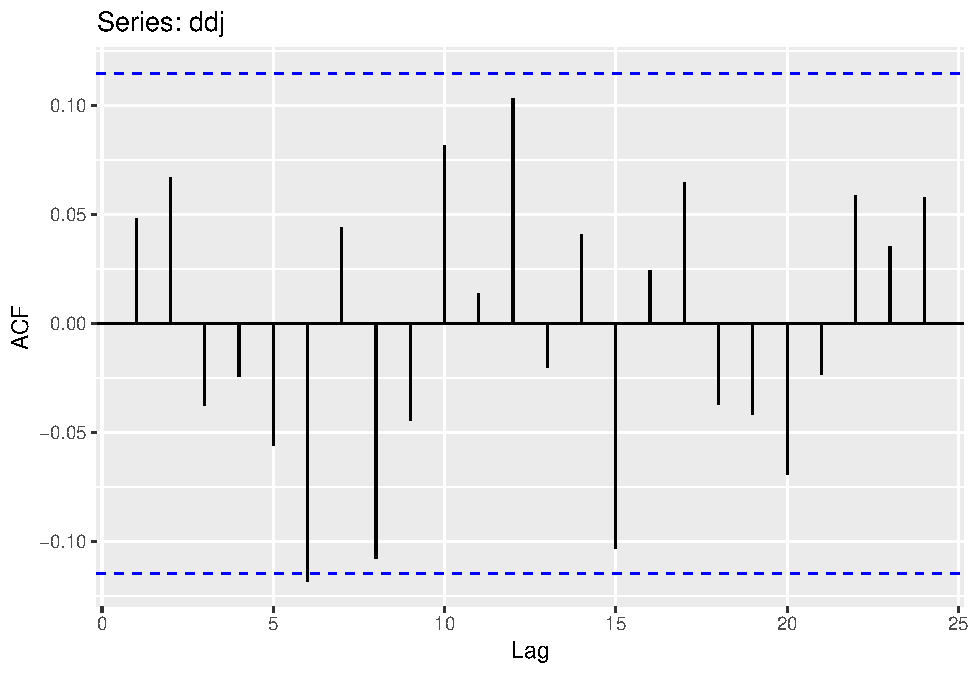
\includegraphics{_main_files/figure-latex/unnamed-chunk-14-1.pdf}

The changes in the Dow Jones Index do appear to be white noise as the the autocorrelations are very close to zero

\hypertarget{section-3}{%
\section{3.1}\label{section-3}}

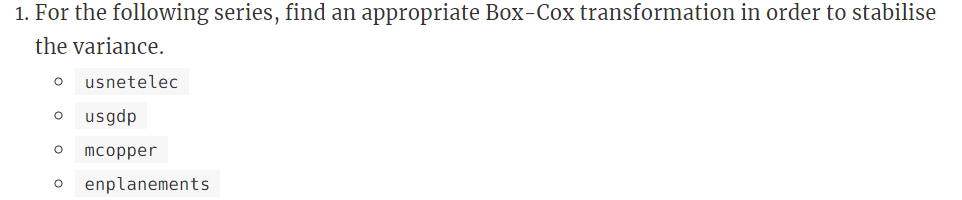
\includegraphics{./week1/3.1.png}

\hypertarget{usnetelec}{%
\subsection{usnetelec}\label{usnetelec}}

\begin{Shaded}
\begin{Highlighting}[]
\KeywordTok{data}\NormalTok{(}\StringTok{"usnetelec"}\NormalTok{)}
\NormalTok{lambda <-}\StringTok{ }\KeywordTok{BoxCox.lambda}\NormalTok{(usnetelec) }\OperatorTok
\StringTok{  }\KeywordTok{print}\NormalTok{()}
\end{Highlighting}
\end{Shaded}

\begin{verbatim}
## [1] 0.5167714
\end{verbatim}

\begin{Shaded}
\begin{Highlighting}[]
\KeywordTok{autoplot}\NormalTok{(}\KeywordTok{BoxCox}\NormalTok{(usnetelec, lambda))}
\end{Highlighting}
\end{Shaded}

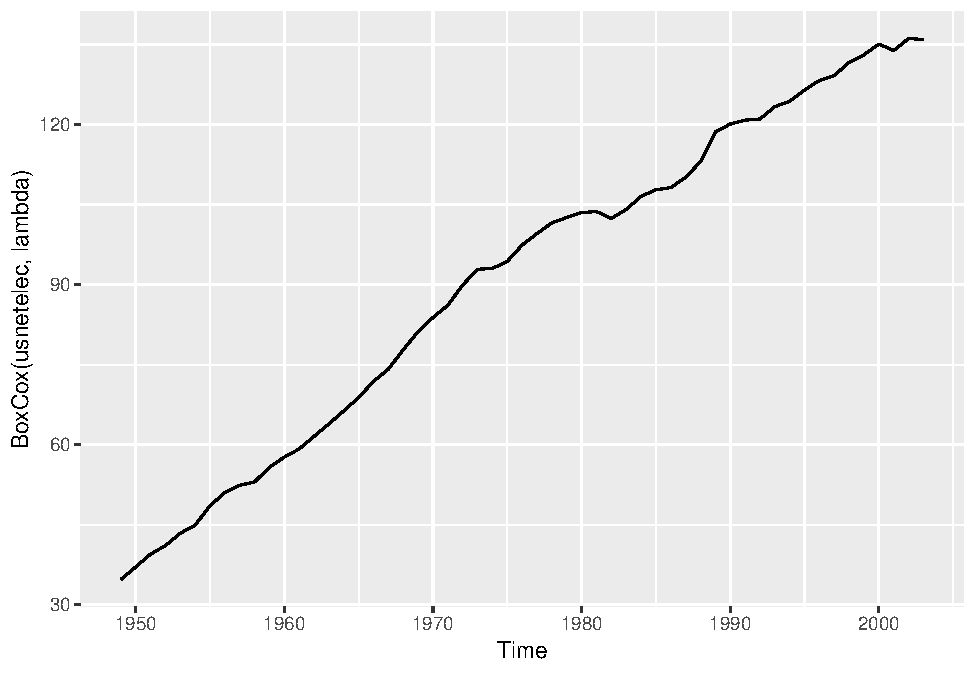
\includegraphics{_main_files/figure-latex/unnamed-chunk-15-1.pdf}

\hypertarget{usgdp}{%
\subsection{usgdp}\label{usgdp}}

\begin{Shaded}
\begin{Highlighting}[]
\KeywordTok{data}\NormalTok{(}\StringTok{"usgdp"}\NormalTok{)}
\NormalTok{lambda <-}\StringTok{ }\KeywordTok{BoxCox.lambda}\NormalTok{(usgdp) }\OperatorTok
\StringTok{  }\KeywordTok{print}\NormalTok{()}
\end{Highlighting}
\end{Shaded}

\begin{verbatim}
## [1] 0.366352
\end{verbatim}

\begin{Shaded}
\begin{Highlighting}[]
\KeywordTok{autoplot}\NormalTok{(}\KeywordTok{BoxCox}\NormalTok{(usgdp, lambda))}
\end{Highlighting}
\end{Shaded}

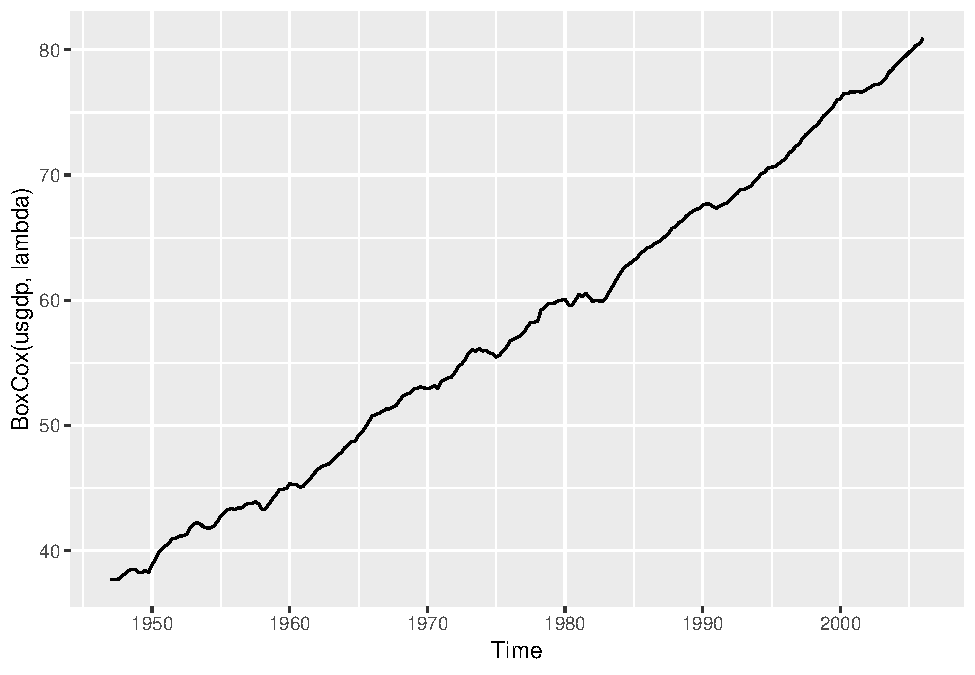
\includegraphics{_main_files/figure-latex/unnamed-chunk-16-1.pdf}

\hypertarget{mcopper}{%
\subsection{mcopper}\label{mcopper}}

\begin{Shaded}
\begin{Highlighting}[]
\KeywordTok{data}\NormalTok{(}\StringTok{"mcopper"}\NormalTok{)}
\NormalTok{lambda <-}\StringTok{ }\KeywordTok{BoxCox.lambda}\NormalTok{(mcopper) }\OperatorTok
\StringTok{  }\KeywordTok{print}\NormalTok{()}
\end{Highlighting}
\end{Shaded}

\begin{verbatim}
## [1] 0.1919047
\end{verbatim}

\begin{Shaded}
\begin{Highlighting}[]
\KeywordTok{autoplot}\NormalTok{(}\KeywordTok{BoxCox}\NormalTok{(mcopper, lambda))}
\end{Highlighting}
\end{Shaded}

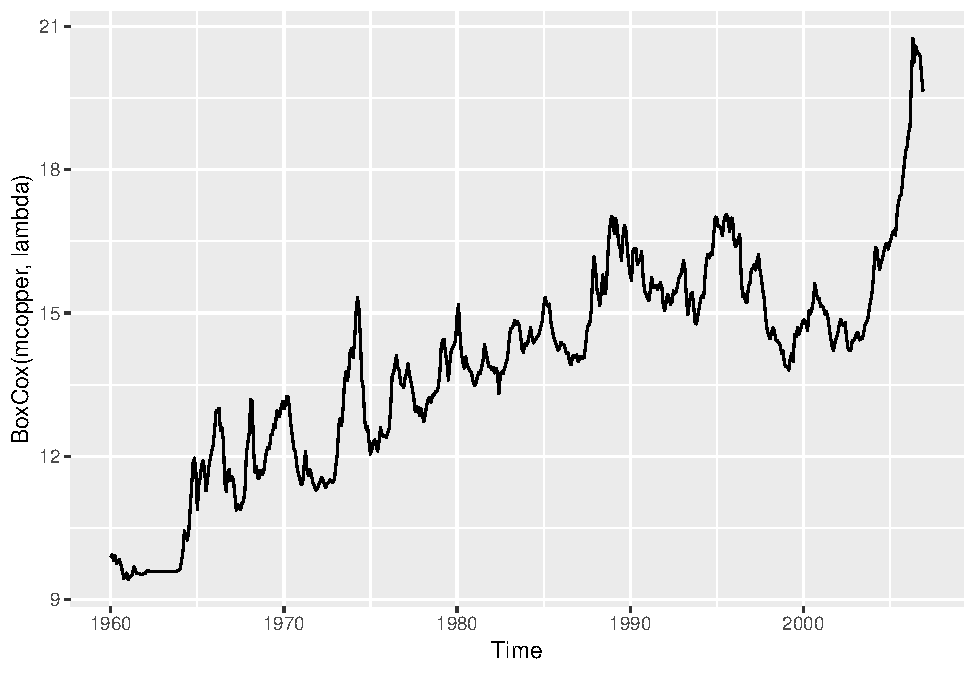
\includegraphics{_main_files/figure-latex/unnamed-chunk-17-1.pdf}

\hypertarget{enplanements}{%
\subsection{enplanements}\label{enplanements}}

\begin{Shaded}
\begin{Highlighting}[]
\KeywordTok{data}\NormalTok{(}\StringTok{"enplanements"}\NormalTok{)}
\NormalTok{lambda <-}\StringTok{ }\KeywordTok{BoxCox.lambda}\NormalTok{(enplanements) }\OperatorTok
\StringTok{  }\KeywordTok{print}\NormalTok{()}
\end{Highlighting}
\end{Shaded}

\begin{verbatim}
## [1] -0.2269461
\end{verbatim}

\begin{Shaded}
\begin{Highlighting}[]
\KeywordTok{autoplot}\NormalTok{(}\KeywordTok{BoxCox}\NormalTok{(enplanements, lambda))}
\end{Highlighting}
\end{Shaded}

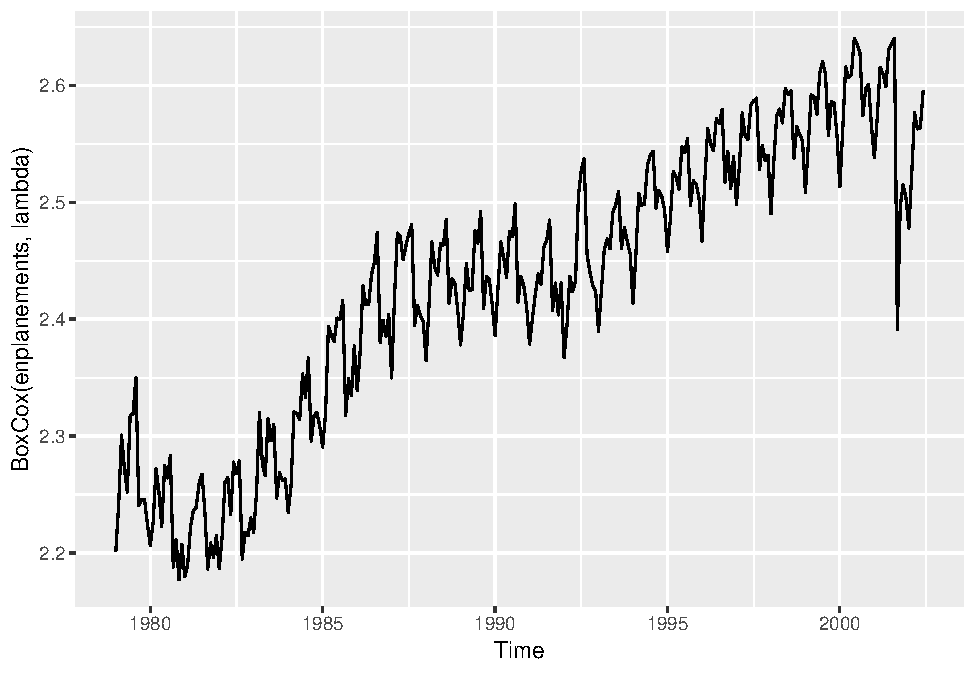
\includegraphics{_main_files/figure-latex/unnamed-chunk-18-1.pdf}

\hypertarget{section-4}{%
\section{3.8}\label{section-4}}

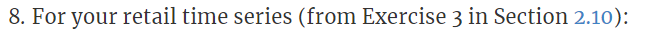
\includegraphics{./week1/3.8.png}

\hypertarget{a-1}{%
\subsection{a}\label{a-1}}

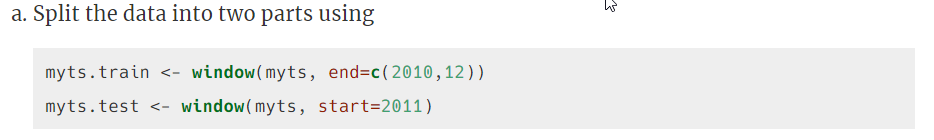
\includegraphics{./week1/3.8a.png}

\begin{Shaded}
\begin{Highlighting}[]
\NormalTok{myts.train <-}\StringTok{ }\KeywordTok{window}\NormalTok{(myts, }\DataTypeTok{end=}\KeywordTok{c}\NormalTok{(}\DecValTok{2010}\NormalTok{,}\DecValTok{12}\NormalTok{))}
\NormalTok{myts.test <-}\StringTok{ }\KeywordTok{window}\NormalTok{(myts, }\DataTypeTok{start=}\DecValTok{2011}\NormalTok{)}
\end{Highlighting}
\end{Shaded}

\hypertarget{b-1}{%
\subsection{b}\label{b-1}}

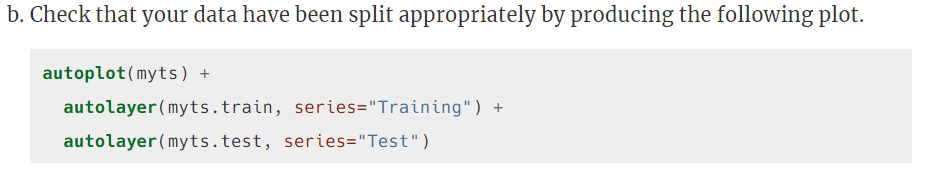
\includegraphics{./week1/3.8b.png}

\begin{Shaded}
\begin{Highlighting}[]
\KeywordTok{autoplot}\NormalTok{(myts) }\OperatorTok{+}
\StringTok{  }\KeywordTok{autolayer}\NormalTok{(myts.train, }\DataTypeTok{series=}\StringTok{"Training"}\NormalTok{) }\OperatorTok{+}
\StringTok{  }\KeywordTok{autolayer}\NormalTok{(myts.test, }\DataTypeTok{series=}\StringTok{"Test"}\NormalTok{)}
\end{Highlighting}
\end{Shaded}

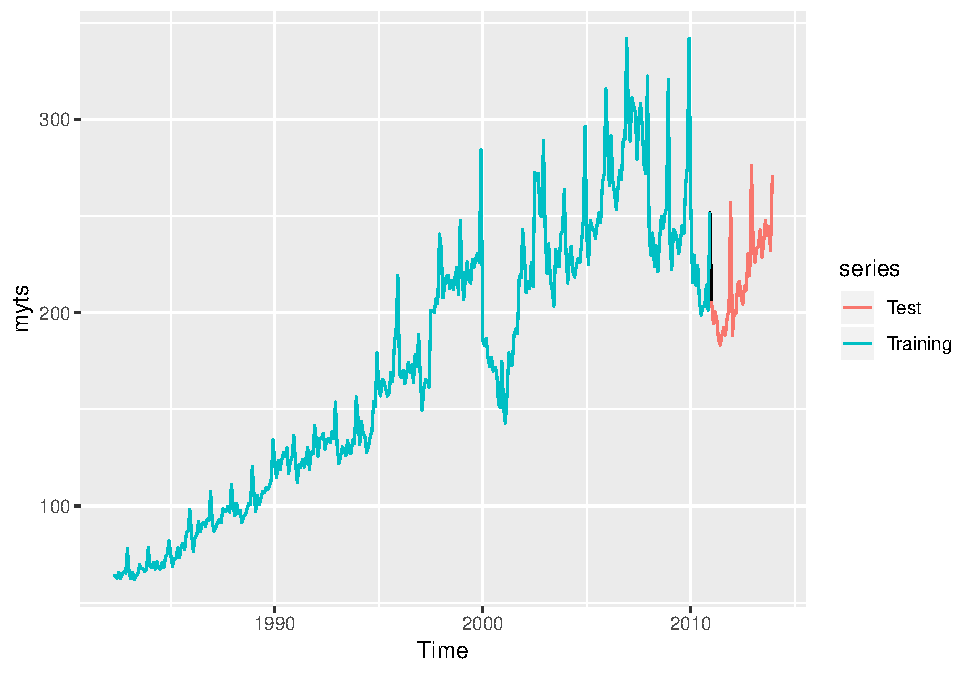
\includegraphics{_main_files/figure-latex/unnamed-chunk-20-1.pdf}

The autoplot shows that the data has been correctly split with the latter part of the data reservered for testing

\hypertarget{c-1}{%
\subsection{c}\label{c-1}}

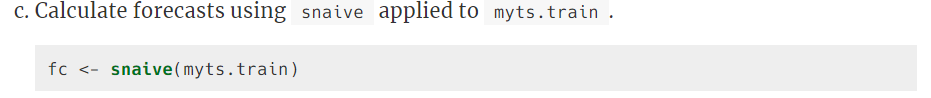
\includegraphics{./week1/3.8c.png}

\begin{Shaded}
\begin{Highlighting}[]
\NormalTok{fc <-}\StringTok{ }\KeywordTok{snaive}\NormalTok{(myts.train)}
\KeywordTok{print}\NormalTok{(fc)}
\end{Highlighting}
\end{Shaded}

\begin{verbatim}
##          Point Forecast    Lo 80    Hi 80    Lo 95    Hi 95
## Jan 2011          255.4 219.8378 290.9622 201.0123 309.7877
## Feb 2011          215.5 179.9378 251.0622 161.1123 269.8877
## Mar 2011          229.6 194.0378 265.1622 175.2123 283.9877
## Apr 2011          214.4 178.8378 249.9622 160.0123 268.7877
## May 2011          224.5 188.9378 260.0622 170.1123 278.8877
## Jun 2011          205.6 170.0378 241.1622 151.2123 259.9877
## Jul 2011          198.7 163.1378 234.2622 144.3123 253.0877
## Aug 2011          203.3 167.7378 238.8622 148.9123 257.6877
## Sep 2011          203.2 167.6378 238.7622 148.8123 257.5877
## Oct 2011          214.4 178.8378 249.9622 160.0123 268.7877
## Nov 2011          201.4 165.8378 236.9622 147.0123 255.7877
## Dec 2011          251.8 216.2378 287.3622 197.4123 306.1877
## Jan 2012          255.4 205.1074 305.6926 178.4841 332.3159
## Feb 2012          215.5 165.2074 265.7926 138.5841 292.4159
## Mar 2012          229.6 179.3074 279.8926 152.6841 306.5159
## Apr 2012          214.4 164.1074 264.6926 137.4841 291.3159
## May 2012          224.5 174.2074 274.7926 147.5841 301.4159
## Jun 2012          205.6 155.3074 255.8926 128.6841 282.5159
## Jul 2012          198.7 148.4074 248.9926 121.7841 275.6159
## Aug 2012          203.3 153.0074 253.5926 126.3841 280.2159
## Sep 2012          203.2 152.9074 253.4926 126.2841 280.1159
## Oct 2012          214.4 164.1074 264.6926 137.4841 291.3159
## Nov 2012          201.4 151.1074 251.6926 124.4841 278.3159
## Dec 2012          251.8 201.5074 302.0926 174.8841 328.7159
\end{verbatim}

\hypertarget{d}{%
\subsection{d}\label{d}}

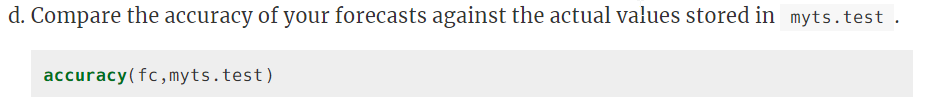
\includegraphics{./week1/3.8d.png}

\begin{Shaded}
\begin{Highlighting}[]
\KeywordTok{accuracy}\NormalTok{(fc, myts.test)}
\end{Highlighting}
\end{Shaded}

\begin{verbatim}
##                      ME     RMSE      MAE       MPE      MAPE     MASE
## Training set   5.502402 27.74935 19.33784  3.369450 10.447161 1.000000
## Test set     -10.845833 24.12202 18.52083 -5.910245  9.201624 0.957751
##                   ACF1 Theil's U
## Training set 0.8703252        NA
## Test set     0.3564215 0.9855325
\end{verbatim}

Conclusions:
* The MASE shows that the seasonal naive method does produce a better forecast than the average naive forecast although very slightly. The MASE is only .95
* The MAPE shows that there is about a 9\% error in the forecast on average which is not bad, but does show tht it could be improved
* The RMSE and MAE both show that it is possible to improve the forecast but the seasonal naive forecast does do a decent job

\hypertarget{e}{%
\subsection{e}\label{e}}

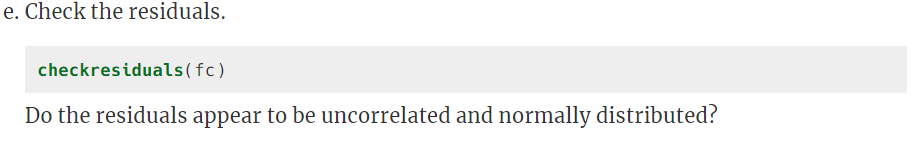
\includegraphics{./week1/3.8e.png}

\begin{Shaded}
\begin{Highlighting}[]
\KeywordTok{checkresiduals}\NormalTok{(fc)}
\end{Highlighting}
\end{Shaded}

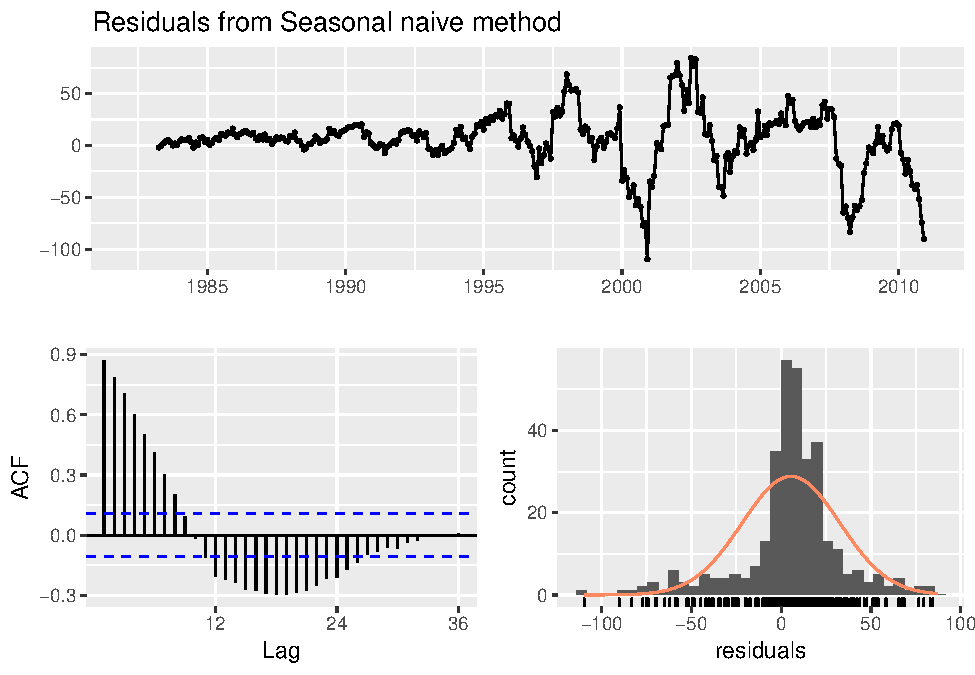
\includegraphics{_main_files/figure-latex/unnamed-chunk-23-1.pdf}

\begin{verbatim}
## 
##  Ljung-Box test
## 
## data:  Residuals from Seasonal naive method
## Q* = 1256.8, df = 24, p-value < 2.2e-16
## 
## Model df: 0.   Total lags used: 24
\end{verbatim}

The residual diagnostics show:
* An approximately normal distribution
* The mean of the residuals is close to 0
* The residual variance appears to be contant
* The residuals appear to be correlated as the lags near to each other are similar in direction and size
* Although the residuals pass the diagnostic tests, it does still show that the prediction intervals may be inaccurate
* The Box-Ljung test does show a very small p-value which means the residuals are distinguishable from a white noise series. The Q* value is also very large

\hypertarget{f}{%
\subsection{f}\label{f}}

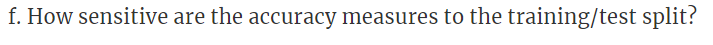
\includegraphics{./week1/3.8f.png}

Accuracy measures are very sensitive to the training/test split. Forecasts by definition need historical data. The more information present

\hypertarget{hw2}{%
\chapter{HW2}\label{hw2}}

\hypertarget{section-5}{%
\section{6.2}\label{section-5}}

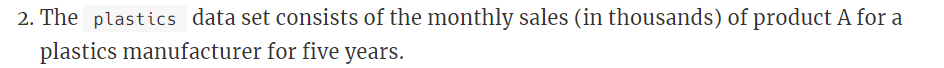
\includegraphics{./week2/6.2.png}

\hypertarget{a-2}{%
\subsection{a}\label{a-2}}

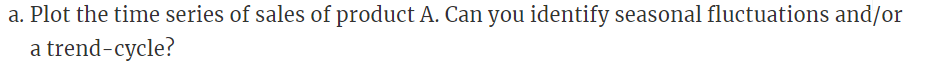
\includegraphics{./week2/6.2a.png}

\begin{Shaded}
\begin{Highlighting}[]
\KeywordTok{autoplot}\NormalTok{(plastics) }\OperatorTok{+}\StringTok{ }\KeywordTok{xlab}\NormalTok{(}\StringTok{"Month"}\NormalTok{) }\OperatorTok{+}\StringTok{ }\KeywordTok{ylab}\NormalTok{(}\StringTok{"1000 $"}\NormalTok{) }\OperatorTok{+}
\StringTok{  }\KeywordTok{ggtitle}\NormalTok{(}\StringTok{"Monthly Plastic Sales"}\NormalTok{)}
\end{Highlighting}
\end{Shaded}

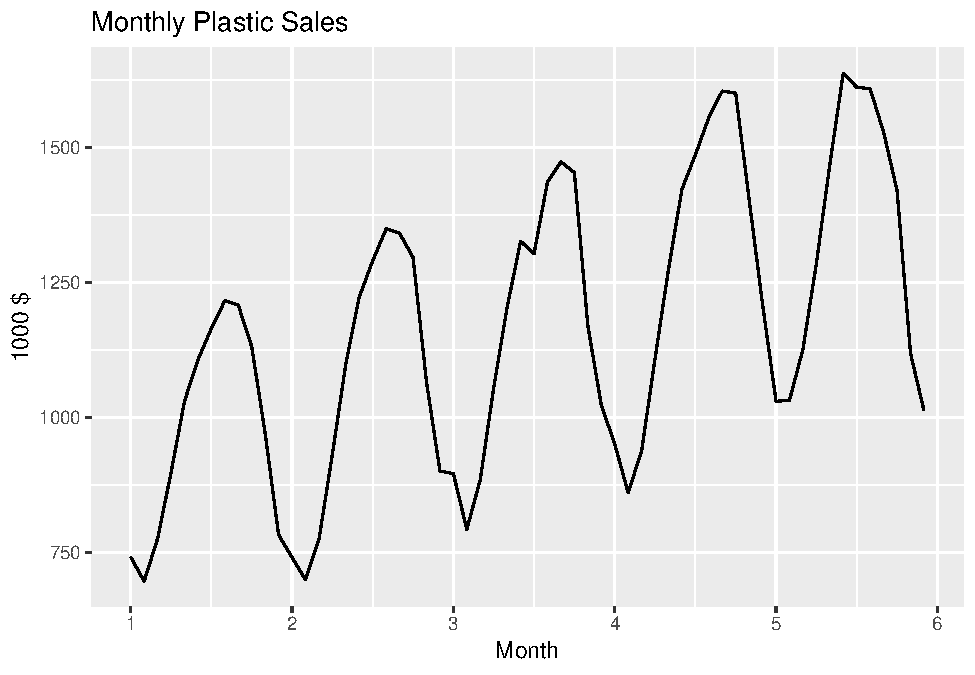
\includegraphics{_main_files/figure-latex/unnamed-chunk-25-1.pdf}

The data has approximately 1 month (peak to peak) seasonality and an apprearent upward trend, that may be cyclic behavior since this only covers 6 months of data.

\hypertarget{b-2}{%
\subsection{b}\label{b-2}}

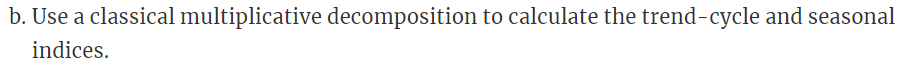
\includegraphics{./week2/6.2b.png}

\begin{Shaded}
\begin{Highlighting}[]
\NormalTok{plastics}
\end{Highlighting}
\end{Shaded}

\begin{verbatim}
##    Jan  Feb  Mar  Apr  May  Jun  Jul  Aug  Sep  Oct  Nov  Dec
## 1  742  697  776  898 1030 1107 1165 1216 1208 1131  971  783
## 2  741  700  774  932 1099 1223 1290 1349 1341 1296 1066  901
## 3  896  793  885 1055 1204 1326 1303 1436 1473 1453 1170 1023
## 4  951  861  938 1109 1274 1422 1486 1555 1604 1600 1403 1209
## 5 1030 1032 1126 1285 1468 1637 1611 1608 1528 1420 1119 1013
\end{verbatim}

\begin{Shaded}
\begin{Highlighting}[]
\KeywordTok{autoplot}\NormalTok{(plastics)}
\end{Highlighting}
\end{Shaded}

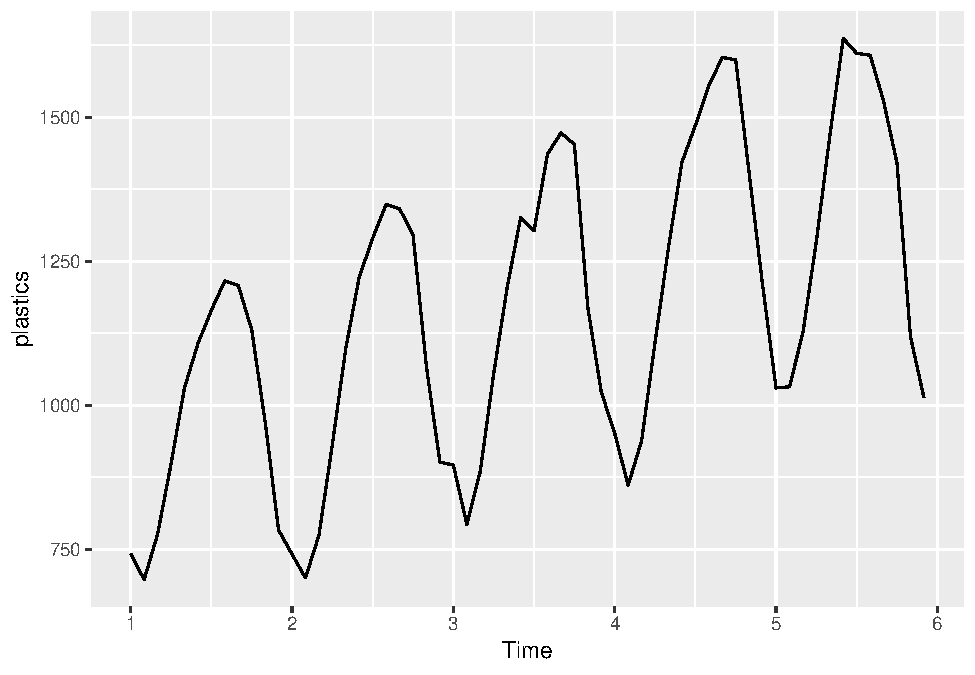
\includegraphics{_main_files/figure-latex/unnamed-chunk-26-1.pdf}

\begin{Shaded}
\begin{Highlighting}[]
\NormalTok{plas_trend <-}\StringTok{ }\KeywordTok{ma}\NormalTok{(plastics, }\DataTypeTok{order =} \DecValTok{12}\NormalTok{, }\DataTypeTok{centre =} \OtherTok{TRUE}\NormalTok{)}
\NormalTok{plas_trend}
\end{Highlighting}
\end{Shaded}

\begin{verbatim}
##         Jan       Feb       Mar       Apr       May       Jun       Jul
## 1        NA        NA        NA        NA        NA        NA  976.9583
## 2 1000.4583 1011.2083 1022.2917 1034.7083 1045.5417 1054.4167 1065.7917
## 3 1117.3750 1121.5417 1130.6667 1142.7083 1153.5833 1163.0000 1170.3750
## 4 1208.7083 1221.2917 1231.7083 1243.2917 1259.1250 1276.5833 1287.6250
## 5 1374.7917 1382.2083 1381.2500 1370.5833 1351.2500 1331.2500        NA
##         Aug       Sep       Oct       Nov       Dec
## 1  977.0417  977.0833  978.4167  982.7083  990.4167
## 2 1076.1250 1084.6250 1094.3750 1103.8750 1112.5417
## 3 1175.5000 1180.5417 1185.0000 1190.1667 1197.0833
## 4 1298.0417 1313.0000 1328.1667 1343.5833 1360.6250
## 5        NA        NA        NA        NA        NA
\end{verbatim}

\begin{Shaded}
\begin{Highlighting}[]
\KeywordTok{autoplot}\NormalTok{(plas_trend)}
\end{Highlighting}
\end{Shaded}

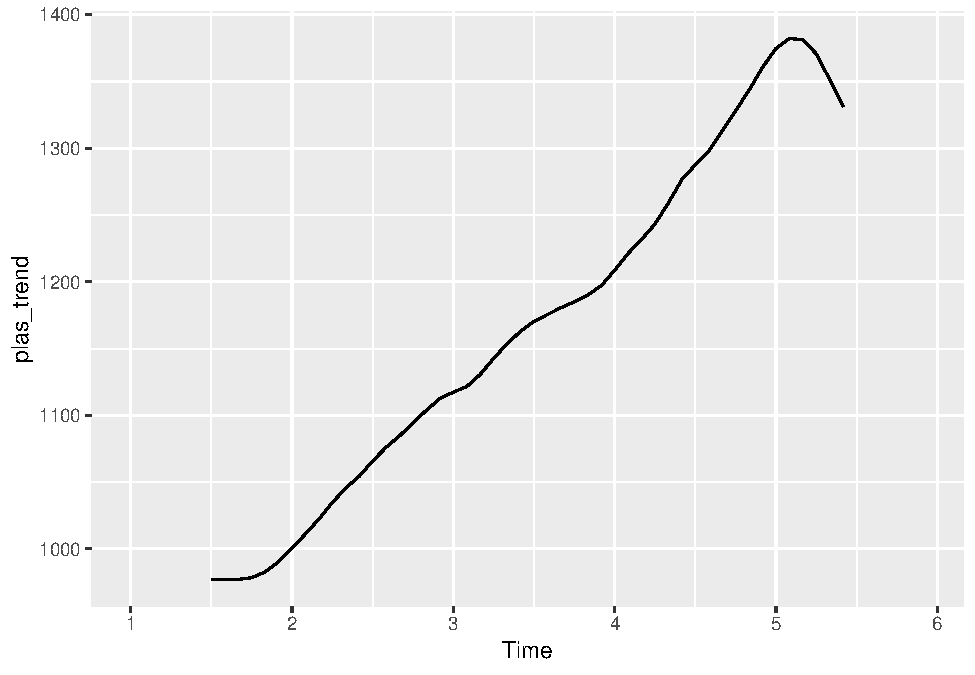
\includegraphics{_main_files/figure-latex/unnamed-chunk-26-2.pdf}

\begin{Shaded}
\begin{Highlighting}[]
\NormalTok{plas_detrend <-}\StringTok{ }\NormalTok{plastics}\OperatorTok{/}\NormalTok{plas_trend}
\NormalTok{plas_detrend}
\end{Highlighting}
\end{Shaded}

\begin{verbatim}
##         Jan       Feb       Mar       Apr       May       Jun       Jul
## 1        NA        NA        NA        NA        NA        NA 1.1924766
## 2 0.7406605 0.6922411 0.7571225 0.9007369 1.0511298 1.1598830 1.2103679
## 3 0.8018794 0.7070625 0.7827241 0.9232452 1.0437044 1.1401548 1.1133184
## 4 0.7867903 0.7049913 0.7615439 0.8919870 1.0118138 1.1139108 1.1540627
## 5 0.7492044 0.7466313 0.8152036 0.9375570 1.0864015 1.2296714        NA
##         Aug       Sep       Oct       Nov       Dec
## 1 1.2445733 1.2363326 1.1559492 0.9880856 0.7905764
## 2 1.2535718 1.2363720 1.1842376 0.9656890 0.8098573
## 3 1.2216078 1.2477323 1.2261603 0.9830556 0.8545771
## 4 1.1979585 1.2216299 1.2046681 1.0442225 0.8885622
## 5        NA        NA        NA        NA        NA
\end{verbatim}

\begin{Shaded}
\begin{Highlighting}[]
\NormalTok{plas_seas <-}\StringTok{ }\KeywordTok{colMeans}\NormalTok{(}\KeywordTok{t}\NormalTok{(}\KeywordTok{matrix}\NormalTok{(plas_detrend,}\DataTypeTok{nrow =} \DecValTok{12}\NormalTok{)), }\DataTypeTok{na.rm =} \OtherTok{TRUE}\NormalTok{)}
\NormalTok{plas_seas}
\end{Highlighting}
\end{Shaded}

\begin{verbatim}
##  [1] 0.7696337 0.7127315 0.7791485 0.9133815 1.0482624 1.1609050 1.1675564
##  [8] 1.2294279 1.2355167 1.1927538 0.9952632 0.8358933
\end{verbatim}

\begin{Shaded}
\begin{Highlighting}[]
\KeywordTok{autoplot}\NormalTok{(}\KeywordTok{as.ts}\NormalTok{(plas_seas))}
\end{Highlighting}
\end{Shaded}

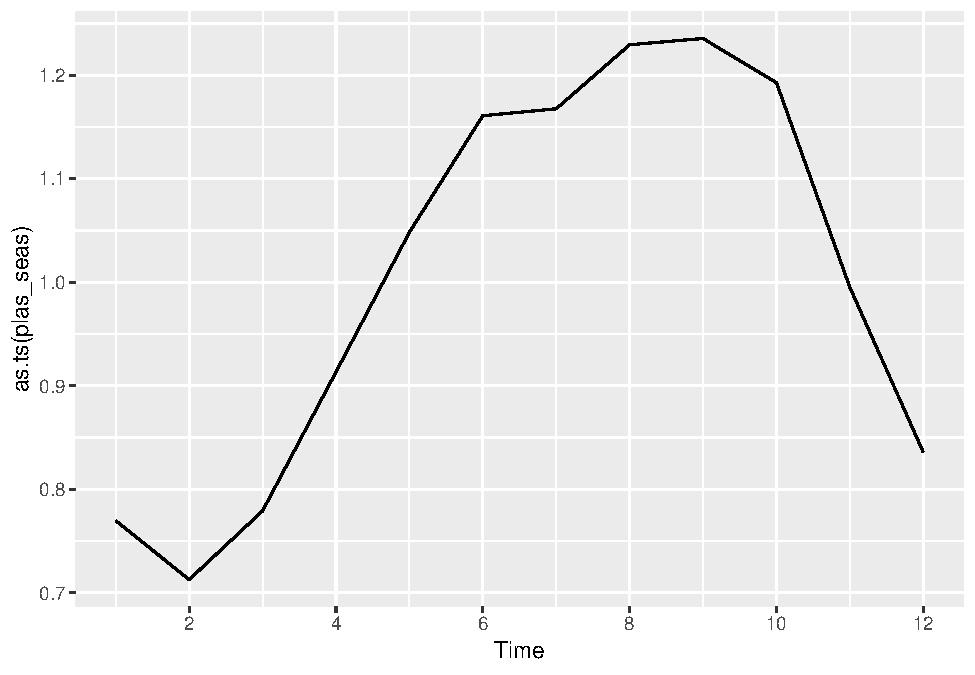
\includegraphics{_main_files/figure-latex/unnamed-chunk-26-3.pdf}

\begin{Shaded}
\begin{Highlighting}[]
\NormalTok{random_plas =}\StringTok{ }\NormalTok{plastics}\OperatorTok{/}\StringTok{ }\NormalTok{(plas_trend}\OperatorTok{*}\StringTok{ }\NormalTok{plas_seas)}
\NormalTok{(random_plas)}
\end{Highlighting}
\end{Shaded}

\begin{verbatim}
##         Jan       Feb       Mar       Apr       May       Jun       Jul
## 1        NA        NA        NA        NA        NA        NA 1.0213439
## 2 0.9623546 0.9712509 0.9717306 0.9861563 1.0027354 0.9991197 1.0366676
## 3 1.0418975 0.9920460 1.0045890 1.0107991 0.9956519 0.9821258 0.9535457
## 4 1.0222920 0.9891400 0.9774053 0.9765766 0.9652295 0.9595194 0.9884428
## 5 0.9734559 1.0475631 1.0462750 1.0264681 1.0363832 1.0592351        NA
##         Aug       Sep       Oct       Nov       Dec
## 1 1.0123191 1.0006604 0.9691432 0.9927883 0.9457863
## 2 1.0196384 1.0006923 0.9928600 0.9702851 0.9688526
## 3 0.9936393 1.0098871 1.0280079 0.9877343 1.0223520
## 4 0.9744032 0.9887603 1.0099889 1.0491923 1.0630092
## 5        NA        NA        NA        NA        NA
\end{verbatim}

\begin{Shaded}
\begin{Highlighting}[]
\NormalTok{random_plas}
\end{Highlighting}
\end{Shaded}

\begin{verbatim}
##         Jan       Feb       Mar       Apr       May       Jun       Jul
## 1        NA        NA        NA        NA        NA        NA 1.0213439
## 2 0.9623546 0.9712509 0.9717306 0.9861563 1.0027354 0.9991197 1.0366676
## 3 1.0418975 0.9920460 1.0045890 1.0107991 0.9956519 0.9821258 0.9535457
## 4 1.0222920 0.9891400 0.9774053 0.9765766 0.9652295 0.9595194 0.9884428
## 5 0.9734559 1.0475631 1.0462750 1.0264681 1.0363832 1.0592351        NA
##         Aug       Sep       Oct       Nov       Dec
## 1 1.0123191 1.0006604 0.9691432 0.9927883 0.9457863
## 2 1.0196384 1.0006923 0.9928600 0.9702851 0.9688526
## 3 0.9936393 1.0098871 1.0280079 0.9877343 1.0223520
## 4 0.9744032 0.9887603 1.0099889 1.0491923 1.0630092
## 5        NA        NA        NA        NA        NA
\end{verbatim}

\begin{Shaded}
\begin{Highlighting}[]
\NormalTok{plastics }\OperatorTok\StringTok{ }\KeywordTok{decompose}\NormalTok{(}\DataTypeTok{type=}\StringTok{"multiplicative"}\NormalTok{) }\OperatorTok
\StringTok{  }\KeywordTok{autoplot}\NormalTok{() }\OperatorTok{+}\StringTok{ }\KeywordTok{xlab}\NormalTok{(}\StringTok{"Month"}\NormalTok{) }\OperatorTok{+}
\StringTok{  }\KeywordTok{ggtitle}\NormalTok{(}\StringTok{"Classical multiplicative decomposition}
\StringTok{    of Plastic Sales"}\NormalTok{)}
\end{Highlighting}
\end{Shaded}

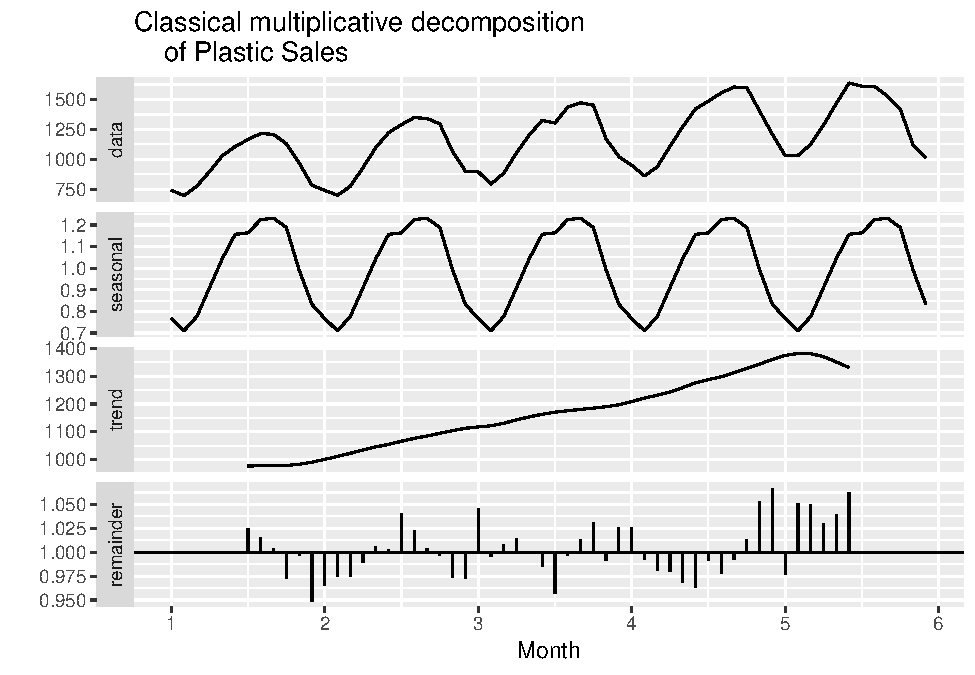
\includegraphics{_main_files/figure-latex/unnamed-chunk-27-1.pdf}

\begin{Shaded}
\begin{Highlighting}[]
\NormalTok{plastics }\OperatorTok\StringTok{ }\KeywordTok{decompose}\NormalTok{(}\DataTypeTok{type=}\StringTok{"multiplicative"}\NormalTok{)}
\end{Highlighting}
\end{Shaded}

\begin{verbatim}
## $x
##    Jan  Feb  Mar  Apr  May  Jun  Jul  Aug  Sep  Oct  Nov  Dec
## 1  742  697  776  898 1030 1107 1165 1216 1208 1131  971  783
## 2  741  700  774  932 1099 1223 1290 1349 1341 1296 1066  901
## 3  896  793  885 1055 1204 1326 1303 1436 1473 1453 1170 1023
## 4  951  861  938 1109 1274 1422 1486 1555 1604 1600 1403 1209
## 5 1030 1032 1126 1285 1468 1637 1611 1608 1528 1420 1119 1013
## 
## $seasonal
##         Jan       Feb       Mar       Apr       May       Jun       Jul
## 1 0.7670466 0.7103357 0.7765294 0.9103112 1.0447386 1.1570026 1.1636317
## 2 0.7670466 0.7103357 0.7765294 0.9103112 1.0447386 1.1570026 1.1636317
## 3 0.7670466 0.7103357 0.7765294 0.9103112 1.0447386 1.1570026 1.1636317
## 4 0.7670466 0.7103357 0.7765294 0.9103112 1.0447386 1.1570026 1.1636317
## 5 0.7670466 0.7103357 0.7765294 0.9103112 1.0447386 1.1570026 1.1636317
##         Aug       Sep       Oct       Nov       Dec
## 1 1.2252952 1.2313635 1.1887444 0.9919176 0.8330834
## 2 1.2252952 1.2313635 1.1887444 0.9919176 0.8330834
## 3 1.2252952 1.2313635 1.1887444 0.9919176 0.8330834
## 4 1.2252952 1.2313635 1.1887444 0.9919176 0.8330834
## 5 1.2252952 1.2313635 1.1887444 0.9919176 0.8330834
## 
## $trend
##         Jan       Feb       Mar       Apr       May       Jun       Jul
## 1        NA        NA        NA        NA        NA        NA  976.9583
## 2 1000.4583 1011.2083 1022.2917 1034.7083 1045.5417 1054.4167 1065.7917
## 3 1117.3750 1121.5417 1130.6667 1142.7083 1153.5833 1163.0000 1170.3750
## 4 1208.7083 1221.2917 1231.7083 1243.2917 1259.1250 1276.5833 1287.6250
## 5 1374.7917 1382.2083 1381.2500 1370.5833 1351.2500 1331.2500        NA
##         Aug       Sep       Oct       Nov       Dec
## 1  977.0417  977.0833  978.4167  982.7083  990.4167
## 2 1076.1250 1084.6250 1094.3750 1103.8750 1112.5417
## 3 1175.5000 1180.5417 1185.0000 1190.1667 1197.0833
## 4 1298.0417 1313.0000 1328.1667 1343.5833 1360.6250
## 5        NA        NA        NA        NA        NA
## 
## $random
##         Jan       Feb       Mar       Apr       May       Jun       Jul
## 1        NA        NA        NA        NA        NA        NA 1.0247887
## 2 0.9656005 0.9745267 0.9750081 0.9894824 1.0061175 1.0024895 1.0401641
## 3 1.0454117 0.9953920 1.0079773 1.0142083 0.9990100 0.9854384 0.9567618
## 4 1.0257400 0.9924762 0.9807020 0.9798704 0.9684851 0.9627557 0.9917766
## 5 0.9767392 1.0510964 1.0498039 1.0299302 1.0398787 1.0628077        NA
##         Aug       Sep       Oct       Nov       Dec
## 1 1.0157335 1.0040354 0.9724119 0.9961368 0.9489762
## 2 1.0230774 1.0040674 0.9962088 0.9735577 0.9721203
## 3 0.9969907 1.0132932 1.0314752 0.9910657 1.0258002
## 4 0.9776897 0.9920952 1.0133954 1.0527311 1.0665946
## 5        NA        NA        NA        NA        NA
## 
## $figure
##  [1] 0.7670466 0.7103357 0.7765294 0.9103112 1.0447386 1.1570026 1.1636317
##  [8] 1.2252952 1.2313635 1.1887444 0.9919176 0.8330834
## 
## $type
## [1] "multiplicative"
## 
## attr(,"class")
## [1] "decomposed.ts"
\end{verbatim}

\hypertarget{c-2}{%
\subsection{c}\label{c-2}}

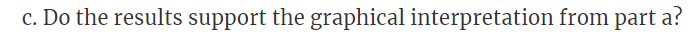
\includegraphics{./week2/6.2c.png}

Yes the trend is sloped upward and the seasonal trend reaches maximum once a month.

\hypertarget{d-1}{%
\subsection{d}\label{d-1}}

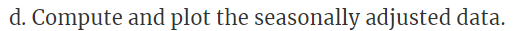
\includegraphics{./week2/6.2d.png}

\begin{Shaded}
\begin{Highlighting}[]
\NormalTok{plas_seas <-}\StringTok{ }\KeywordTok{decompose}\NormalTok{(plastics, }\DataTypeTok{type =} \StringTok{'multiplicative'}\NormalTok{)}\OperatorTok{$}\NormalTok{seasonal}
\NormalTok{plas_seas}
\end{Highlighting}
\end{Shaded}

\begin{verbatim}
##         Jan       Feb       Mar       Apr       May       Jun       Jul
## 1 0.7670466 0.7103357 0.7765294 0.9103112 1.0447386 1.1570026 1.1636317
## 2 0.7670466 0.7103357 0.7765294 0.9103112 1.0447386 1.1570026 1.1636317
## 3 0.7670466 0.7103357 0.7765294 0.9103112 1.0447386 1.1570026 1.1636317
## 4 0.7670466 0.7103357 0.7765294 0.9103112 1.0447386 1.1570026 1.1636317
## 5 0.7670466 0.7103357 0.7765294 0.9103112 1.0447386 1.1570026 1.1636317
##         Aug       Sep       Oct       Nov       Dec
## 1 1.2252952 1.2313635 1.1887444 0.9919176 0.8330834
## 2 1.2252952 1.2313635 1.1887444 0.9919176 0.8330834
## 3 1.2252952 1.2313635 1.1887444 0.9919176 0.8330834
## 4 1.2252952 1.2313635 1.1887444 0.9919176 0.8330834
## 5 1.2252952 1.2313635 1.1887444 0.9919176 0.8330834
\end{verbatim}

\begin{Shaded}
\begin{Highlighting}[]
\NormalTok{plas_seas_adj =}\StringTok{ }\NormalTok{plastics}\OperatorTok{/}\NormalTok{plas_seas}
\KeywordTok{autoplot}\NormalTok{(plas_seas_adj)}
\end{Highlighting}
\end{Shaded}

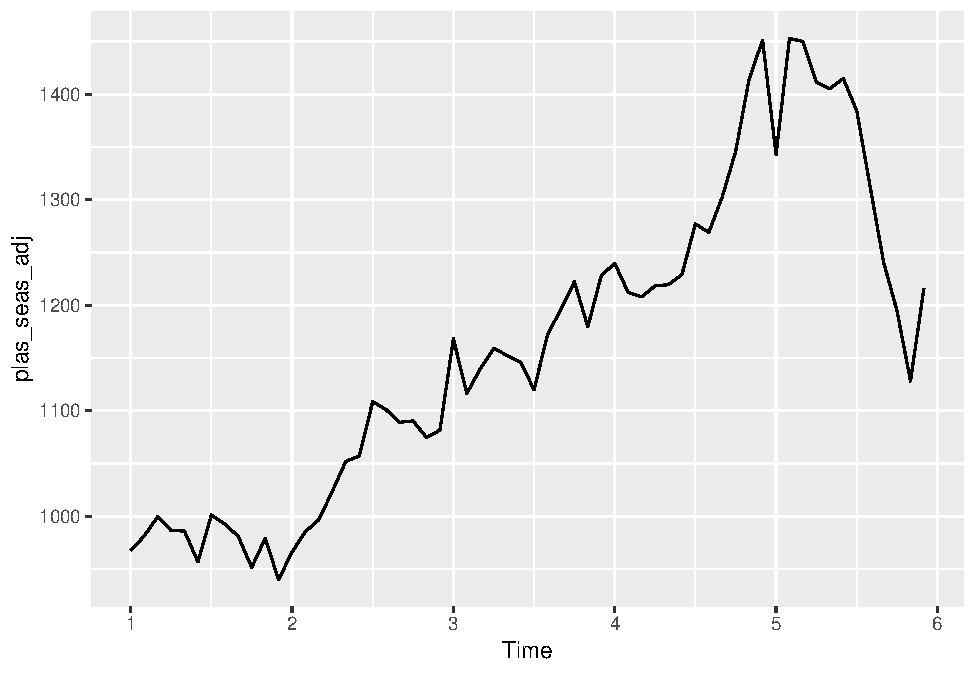
\includegraphics{_main_files/figure-latex/unnamed-chunk-29-1.pdf}

\hypertarget{e-1}{%
\subsection{e}\label{e-1}}

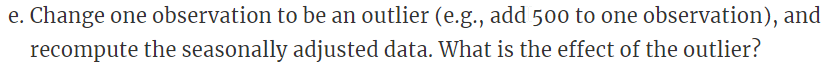
\includegraphics{./week2/6.2e.png}

\begin{Shaded}
\begin{Highlighting}[]
\NormalTok{plastics[}\DecValTok{30}\NormalTok{]}
\end{Highlighting}
\end{Shaded}

\begin{verbatim}
## [1] 1326
\end{verbatim}

\begin{Shaded}
\begin{Highlighting}[]
\NormalTok{new_val <-}\StringTok{ }\NormalTok{plastics[}\DecValTok{30}\NormalTok{]}\OperatorTok{+}\DecValTok{500}
\NormalTok{plas_outlier <-}\StringTok{ }\KeywordTok{replace}\NormalTok{(plastics,}\DecValTok{30}\NormalTok{, new_val)}
\NormalTok{plas_outlier[}\DecValTok{30}\NormalTok{]}
\end{Highlighting}
\end{Shaded}

\begin{verbatim}
## [1] 1826
\end{verbatim}

\begin{Shaded}
\begin{Highlighting}[]
\NormalTok{plas_seas_outlier <-}\StringTok{ }\KeywordTok{decompose}\NormalTok{(plas_outlier, }\DataTypeTok{type =} \StringTok{'multiplicative'}\NormalTok{)}\OperatorTok{$}\NormalTok{seasonal}
\NormalTok{plas_seas_outlier}
\end{Highlighting}
\end{Shaded}

\begin{verbatim}
##         Jan       Feb       Mar       Apr       May       Jun       Jul
## 1 0.7598996 0.7040581 0.7696340 0.9022607 1.0357218 1.2506498 1.1541497
## 2 0.7598996 0.7040581 0.7696340 0.9022607 1.0357218 1.2506498 1.1541497
## 3 0.7598996 0.7040581 0.7696340 0.9022607 1.0357218 1.2506498 1.1541497
## 4 0.7598996 0.7040581 0.7696340 0.9022607 1.0357218 1.2506498 1.1541497
## 5 0.7598996 0.7040581 0.7696340 0.9022607 1.0357218 1.2506498 1.1541497
##         Aug       Sep       Oct       Nov       Dec
## 1 1.2149325 1.2208222 1.1784222 0.9836787 0.8257707
## 2 1.2149325 1.2208222 1.1784222 0.9836787 0.8257707
## 3 1.2149325 1.2208222 1.1784222 0.9836787 0.8257707
## 4 1.2149325 1.2208222 1.1784222 0.9836787 0.8257707
## 5 1.2149325 1.2208222 1.1784222 0.9836787 0.8257707
\end{verbatim}

\begin{Shaded}
\begin{Highlighting}[]
\NormalTok{plas_seas_adj_outlier =}\StringTok{ }\NormalTok{plas_outlier}\OperatorTok{/}\NormalTok{plas_seas_outlier}
\KeywordTok{autoplot}\NormalTok{(plas_seas_adj_outlier)}
\end{Highlighting}
\end{Shaded}

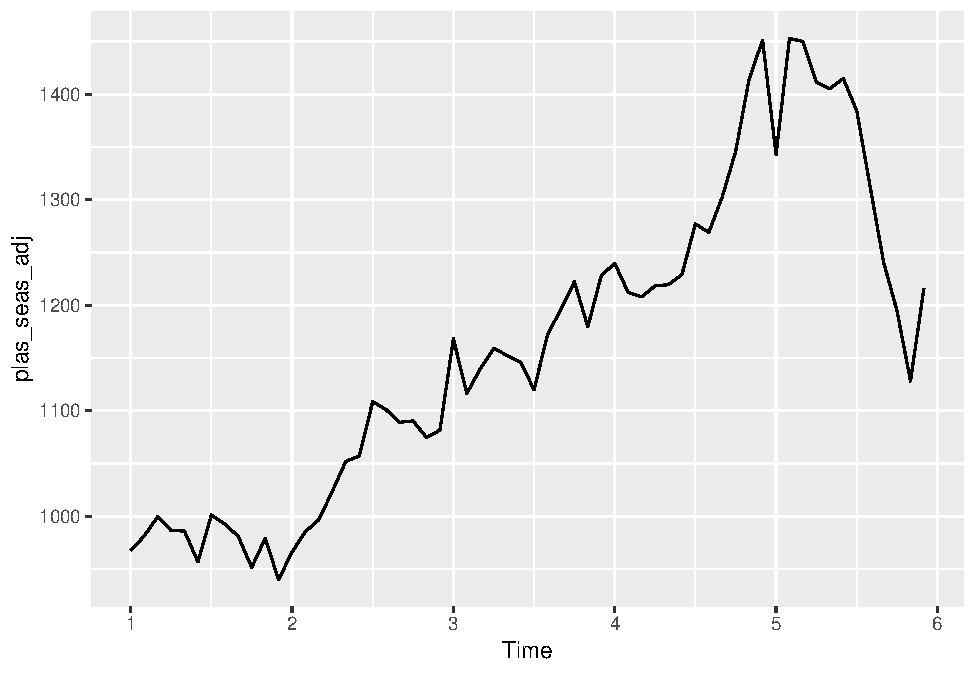
\includegraphics{_main_files/figure-latex/unnamed-chunk-30-1.pdf}

It adds a spike to the seasonally adjusted data where the outlier is.

\hypertarget{f-1}{%
\subsection{f}\label{f-1}}

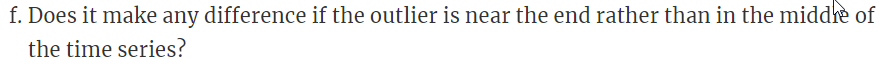
\includegraphics{./week2/6.2f.png}

\begin{Shaded}
\begin{Highlighting}[]
\NormalTok{plastics[}\DecValTok{5}\NormalTok{]}
\end{Highlighting}
\end{Shaded}

\begin{verbatim}
## [1] 1030
\end{verbatim}

\begin{Shaded}
\begin{Highlighting}[]
\NormalTok{new_val <-}\StringTok{ }\NormalTok{plastics[}\DecValTok{5}\NormalTok{]}\OperatorTok{+}\DecValTok{500}
\NormalTok{plas_outlier <-}\StringTok{ }\KeywordTok{replace}\NormalTok{(plastics,}\DecValTok{5}\NormalTok{, new_val)}
\NormalTok{plas_outlier[}\DecValTok{5}\NormalTok{]}
\end{Highlighting}
\end{Shaded}

\begin{verbatim}
## [1] 1530
\end{verbatim}

\begin{Shaded}
\begin{Highlighting}[]
\NormalTok{plas_seas_outlier <-}\StringTok{ }\KeywordTok{decompose}\NormalTok{(plas_outlier, }\DataTypeTok{type =} \StringTok{'multiplicative'}\NormalTok{)}\OperatorTok{$}\NormalTok{seasonal}
\NormalTok{plas_seas_outlier}
\end{Highlighting}
\end{Shaded}

\begin{verbatim}
##         Jan       Feb       Mar       Apr       May       Jun       Jul
## 1 0.7705339 0.7135653 0.7800599 0.9144500 1.0494886 1.1622630 1.1567134
## 2 0.7705339 0.7135653 0.7800599 0.9144500 1.0494886 1.1622630 1.1567134
## 3 0.7705339 0.7135653 0.7800599 0.9144500 1.0494886 1.1622630 1.1567134
## 4 0.7705339 0.7135653 0.7800599 0.9144500 1.0494886 1.1622630 1.1567134
## 5 0.7705339 0.7135653 0.7800599 0.9144500 1.0494886 1.1622630 1.1567134
##         Aug       Sep       Oct       Nov       Dec
## 1 1.2181249 1.2243057 1.1823311 0.9912933 0.8368710
## 2 1.2181249 1.2243057 1.1823311 0.9912933 0.8368710
## 3 1.2181249 1.2243057 1.1823311 0.9912933 0.8368710
## 4 1.2181249 1.2243057 1.1823311 0.9912933 0.8368710
## 5 1.2181249 1.2243057 1.1823311 0.9912933 0.8368710
\end{verbatim}

\begin{Shaded}
\begin{Highlighting}[]
\NormalTok{plas_seas_adj_outlier =}\StringTok{ }\NormalTok{plas_outlier}\OperatorTok{/}\NormalTok{plas_seas_outlier}
\KeywordTok{autoplot}\NormalTok{(plas_seas_adj_outlier)}
\end{Highlighting}
\end{Shaded}

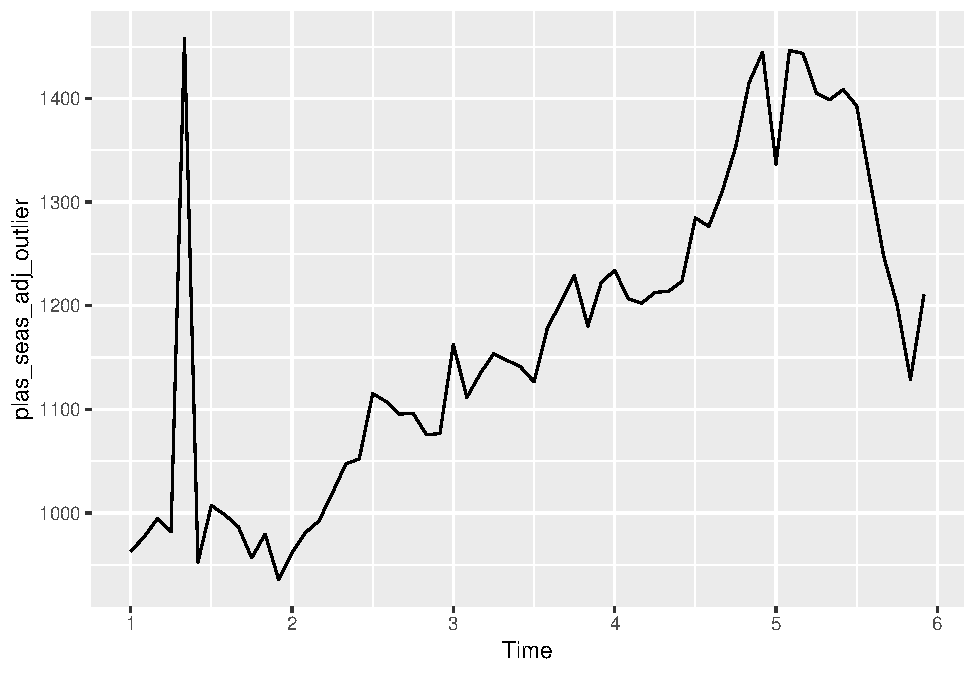
\includegraphics{_main_files/figure-latex/unnamed-chunk-31-1.pdf}

\begin{Shaded}
\begin{Highlighting}[]
\NormalTok{plastics[}\DecValTok{55}\NormalTok{]}
\end{Highlighting}
\end{Shaded}

\begin{verbatim}
## [1] 1611
\end{verbatim}

\begin{Shaded}
\begin{Highlighting}[]
\NormalTok{new_val <-}\StringTok{ }\NormalTok{plastics[}\DecValTok{55}\NormalTok{]}\OperatorTok{+}\DecValTok{500}
\NormalTok{plas_outlier <-}\StringTok{ }\KeywordTok{replace}\NormalTok{(plastics,}\DecValTok{55}\NormalTok{, new_val)}
\NormalTok{plas_outlier[}\DecValTok{55}\NormalTok{]}
\end{Highlighting}
\end{Shaded}

\begin{verbatim}
## [1] 2111
\end{verbatim}

\begin{Shaded}
\begin{Highlighting}[]
\NormalTok{plas_seas_outlier <-}\StringTok{ }\KeywordTok{decompose}\NormalTok{(plas_outlier, }\DataTypeTok{type =} \StringTok{'multiplicative'}\NormalTok{)}\OperatorTok{$}\NormalTok{seasonal}
\NormalTok{plas_seas_outlier}
\end{Highlighting}
\end{Shaded}

\begin{verbatim}
##         Jan       Feb       Mar       Apr       May       Jun       Jul
## 1 0.7667177 0.7071587 0.7730597 0.9063243 1.0399751 1.1513949 1.1673737
## 2 0.7667177 0.7071587 0.7730597 0.9063243 1.0399751 1.1513949 1.1673737
## 3 0.7667177 0.7071587 0.7730597 0.9063243 1.0399751 1.1513949 1.1673737
## 4 0.7667177 0.7071587 0.7730597 0.9063243 1.0399751 1.1513949 1.1673737
## 5 0.7667177 0.7071587 0.7730597 0.9063243 1.0399751 1.1513949 1.1673737
##         Aug       Sep       Oct       Nov       Dec
## 1 1.2292355 1.2353233 1.1925671 0.9951074 0.8357624
## 2 1.2292355 1.2353233 1.1925671 0.9951074 0.8357624
## 3 1.2292355 1.2353233 1.1925671 0.9951074 0.8357624
## 4 1.2292355 1.2353233 1.1925671 0.9951074 0.8357624
## 5 1.2292355 1.2353233 1.1925671 0.9951074 0.8357624
\end{verbatim}

\begin{Shaded}
\begin{Highlighting}[]
\NormalTok{plas_seas_adj_outlier =}\StringTok{ }\NormalTok{plas_outlier}\OperatorTok{/}\NormalTok{plas_seas_outlier}
\KeywordTok{autoplot}\NormalTok{(plas_seas_adj_outlier)}
\end{Highlighting}
\end{Shaded}

\includegraphics{_main_files/figure-latex/unnamed-chunk-32-1.pdf}

Yes, the spike occurs where the outlier is.

\hypertarget{section-6}{%
\section{6.6}\label{section-6}}

\includegraphics{./week2/6.6.png}

\hypertarget{a-3}{%
\subsection{a}\label{a-3}}

\includegraphics{./week2/6.6a.png}

\begin{Shaded}
\begin{Highlighting}[]
\NormalTok{bricksq }\OperatorTok\StringTok{ }\KeywordTok{autoplot}\NormalTok{()}
\end{Highlighting}
\end{Shaded}

\includegraphics{_main_files/figure-latex/unnamed-chunk-33-1.pdf}

\begin{Shaded}
\begin{Highlighting}[]
\NormalTok{bricksq }\OperatorTok
\StringTok{  }\KeywordTok{stl}\NormalTok{(}\DataTypeTok{t.window=}\DecValTok{13}\NormalTok{, }\DataTypeTok{s.window=}\StringTok{"periodic"}\NormalTok{, }\DataTypeTok{robust=}\OtherTok{TRUE}\NormalTok{) }\OperatorTok
\StringTok{  }\KeywordTok{autoplot}\NormalTok{()}
\end{Highlighting}
\end{Shaded}

\includegraphics{_main_files/figure-latex/unnamed-chunk-33-2.pdf}

\begin{Shaded}
\begin{Highlighting}[]
\NormalTok{bricksq }\OperatorTok
\StringTok{  }\KeywordTok{stl}\NormalTok{(}\DataTypeTok{t.window=}\DecValTok{13}\NormalTok{, }\DataTypeTok{s.window=}\DecValTok{7}\NormalTok{, }\DataTypeTok{robust=}\OtherTok{TRUE}\NormalTok{) }\OperatorTok
\StringTok{  }\KeywordTok{autoplot}\NormalTok{()}
\end{Highlighting}
\end{Shaded}

\includegraphics{_main_files/figure-latex/unnamed-chunk-33-3.pdf}

\begin{Shaded}
\begin{Highlighting}[]
\NormalTok{bricksq }\OperatorTok
\StringTok{  }\KeywordTok{stl}\NormalTok{(}\DataTypeTok{t.window=}\DecValTok{13}\NormalTok{, }\DataTypeTok{s.window=}\DecValTok{25}\NormalTok{, }\DataTypeTok{robust=}\OtherTok{TRUE}\NormalTok{) }\OperatorTok
\StringTok{  }\KeywordTok{autoplot}\NormalTok{()}
\end{Highlighting}
\end{Shaded}

\includegraphics{_main_files/figure-latex/unnamed-chunk-33-4.pdf}

\begin{Shaded}
\begin{Highlighting}[]
\NormalTok{bricksq }\OperatorTok
\StringTok{  }\KeywordTok{stl}\NormalTok{(}\DataTypeTok{t.window=}\DecValTok{13}\NormalTok{, }\DataTypeTok{s.window=}\DecValTok{81}\NormalTok{, }\DataTypeTok{robust=}\OtherTok{TRUE}\NormalTok{) }\OperatorTok
\StringTok{  }\KeywordTok{autoplot}\NormalTok{()}
\end{Highlighting}
\end{Shaded}

\includegraphics{_main_files/figure-latex/unnamed-chunk-33-5.pdf}

We see that a high s.window yeilds the same as periodic.

\begin{Shaded}
\begin{Highlighting}[]
\NormalTok{bricksq }\OperatorTok\StringTok{ }\KeywordTok{autoplot}\NormalTok{()}
\end{Highlighting}
\end{Shaded}

\includegraphics{_main_files/figure-latex/unnamed-chunk-34-1.pdf}

\begin{Shaded}
\begin{Highlighting}[]
\NormalTok{bricksq }\OperatorTok
\StringTok{  }\KeywordTok{stl}\NormalTok{(}\DataTypeTok{t.window=}\DecValTok{13}\NormalTok{, }\DataTypeTok{s.window=}\StringTok{"periodic"}\NormalTok{, }\DataTypeTok{robust=}\OtherTok{TRUE}\NormalTok{) }\OperatorTok
\StringTok{  }\KeywordTok{autoplot}\NormalTok{()}
\end{Highlighting}
\end{Shaded}

\includegraphics{_main_files/figure-latex/unnamed-chunk-34-2.pdf}

\begin{Shaded}
\begin{Highlighting}[]
\NormalTok{bricksq }\OperatorTok
\StringTok{  }\KeywordTok{stl}\NormalTok{(}\DataTypeTok{t.window=}\DecValTok{25}\NormalTok{, }\DataTypeTok{s.window=}\StringTok{"periodic"}\NormalTok{, }\DataTypeTok{robust=}\OtherTok{TRUE}\NormalTok{) }\OperatorTok
\StringTok{  }\KeywordTok{autoplot}\NormalTok{()}
\end{Highlighting}
\end{Shaded}

\includegraphics{_main_files/figure-latex/unnamed-chunk-34-3.pdf}

\begin{Shaded}
\begin{Highlighting}[]
\NormalTok{bricksq }\OperatorTok
\StringTok{  }\KeywordTok{stl}\NormalTok{(}\DataTypeTok{t.window=}\DecValTok{7}\NormalTok{, }\DataTypeTok{s.window=}\StringTok{"periodic"}\NormalTok{, }\DataTypeTok{robust=}\OtherTok{TRUE}\NormalTok{) }\OperatorTok
\StringTok{  }\KeywordTok{autoplot}\NormalTok{()}
\end{Highlighting}
\end{Shaded}

\includegraphics{_main_files/figure-latex/unnamed-chunk-34-4.pdf}

\begin{Shaded}
\begin{Highlighting}[]
\NormalTok{bricksq }\OperatorTok
\StringTok{  }\KeywordTok{stl}\NormalTok{(}\DataTypeTok{t.window=}\DecValTok{3}\NormalTok{, }\DataTypeTok{s.window=}\StringTok{"periodic"}\NormalTok{, }\DataTypeTok{robust=}\OtherTok{TRUE}\NormalTok{) }\OperatorTok
\StringTok{  }\KeywordTok{autoplot}\NormalTok{()}
\end{Highlighting}
\end{Shaded}

\includegraphics{_main_files/figure-latex/unnamed-chunk-34-5.pdf}

The t.window parameter adjusts the goodness of fit of the trend, low values tend to under fit the trend, and high values tend to over fit the trend.

\hypertarget{b-3}{%
\subsection{b}\label{b-3}}

\includegraphics{./week2/6.6b.png}

\begin{Shaded}
\begin{Highlighting}[]
\NormalTok{brick_seas <-}\StringTok{ }\KeywordTok{decompose}\NormalTok{(bricksq, }\DataTypeTok{type =} \StringTok{'multiplicative'}\NormalTok{)}\OperatorTok{$}\NormalTok{seasonal}
\NormalTok{brick_seas}
\end{Highlighting}
\end{Shaded}

\begin{verbatim}
##          Qtr1     Qtr2     Qtr3     Qtr4
## 1956 0.907788 1.027191 1.061155 1.003866
## 1957 0.907788 1.027191 1.061155 1.003866
## 1958 0.907788 1.027191 1.061155 1.003866
## 1959 0.907788 1.027191 1.061155 1.003866
## 1960 0.907788 1.027191 1.061155 1.003866
## 1961 0.907788 1.027191 1.061155 1.003866
## 1962 0.907788 1.027191 1.061155 1.003866
## 1963 0.907788 1.027191 1.061155 1.003866
## 1964 0.907788 1.027191 1.061155 1.003866
## 1965 0.907788 1.027191 1.061155 1.003866
## 1966 0.907788 1.027191 1.061155 1.003866
## 1967 0.907788 1.027191 1.061155 1.003866
## 1968 0.907788 1.027191 1.061155 1.003866
## 1969 0.907788 1.027191 1.061155 1.003866
## 1970 0.907788 1.027191 1.061155 1.003866
## 1971 0.907788 1.027191 1.061155 1.003866
## 1972 0.907788 1.027191 1.061155 1.003866
## 1973 0.907788 1.027191 1.061155 1.003866
## 1974 0.907788 1.027191 1.061155 1.003866
## 1975 0.907788 1.027191 1.061155 1.003866
## 1976 0.907788 1.027191 1.061155 1.003866
## 1977 0.907788 1.027191 1.061155 1.003866
## 1978 0.907788 1.027191 1.061155 1.003866
## 1979 0.907788 1.027191 1.061155 1.003866
## 1980 0.907788 1.027191 1.061155 1.003866
## 1981 0.907788 1.027191 1.061155 1.003866
## 1982 0.907788 1.027191 1.061155 1.003866
## 1983 0.907788 1.027191 1.061155 1.003866
## 1984 0.907788 1.027191 1.061155 1.003866
## 1985 0.907788 1.027191 1.061155 1.003866
## 1986 0.907788 1.027191 1.061155 1.003866
## 1987 0.907788 1.027191 1.061155 1.003866
## 1988 0.907788 1.027191 1.061155 1.003866
## 1989 0.907788 1.027191 1.061155 1.003866
## 1990 0.907788 1.027191 1.061155 1.003866
## 1991 0.907788 1.027191 1.061155 1.003866
## 1992 0.907788 1.027191 1.061155 1.003866
## 1993 0.907788 1.027191 1.061155 1.003866
## 1994 0.907788 1.027191 1.061155
\end{verbatim}

\begin{Shaded}
\begin{Highlighting}[]
\NormalTok{brick_seas_adj =}\StringTok{ }\NormalTok{bricksq}\OperatorTok{/}\NormalTok{brick_seas}
\KeywordTok{autoplot}\NormalTok{(brick_seas_adj)}
\end{Highlighting}
\end{Shaded}

\includegraphics{_main_files/figure-latex/unnamed-chunk-35-1.pdf}

\hypertarget{c-3}{%
\subsection{c}\label{c-3}}

\includegraphics{./week2/6.6c.png}

\begin{Shaded}
\begin{Highlighting}[]
\NormalTok{brick_naive <-}\StringTok{ }\KeywordTok{naive}\NormalTok{(brick_seas_adj, }\DataTypeTok{h=}\DecValTok{12}\NormalTok{)}
\NormalTok{brick_naive}
\end{Highlighting}
\end{Shaded}

\begin{verbatim}
##         Point Forecast    Lo 80    Hi 80    Lo 95    Hi 95
## 1994 Q4       465.5304 438.0189 493.0419 423.4551 507.6056
## 1995 Q1       465.5304 426.6232 504.4375 406.0270 525.0337
## 1995 Q2       465.5304 417.8790 513.1817 392.6539 538.4068
## 1995 Q3       465.5304 410.5073 520.5534 381.3799 549.6808
## 1995 Q4       465.5304 404.0128 527.0480 371.4473 559.6134
## 1996 Q1       465.5304 398.1412 532.9195 362.4675 568.5932
## 1996 Q2       465.5304 392.7417 538.3190 354.2098 576.8509
## 1996 Q3       465.5304 387.7161 543.3447 346.5237 584.5371
## 1996 Q4       465.5304 382.9958 548.0649 339.3047 591.7560
## 1997 Q1       465.5304 378.5313 552.5294 332.4768 598.5839
## 1997 Q2       465.5304 374.2850 556.7757 325.9826 605.0781
## 1997 Q3       465.5304 370.2277 560.8330 319.7775 611.2832
\end{verbatim}

\begin{Shaded}
\begin{Highlighting}[]
\KeywordTok{autoplot}\NormalTok{(brick_seas_adj) }\OperatorTok{+}
\StringTok{  }\KeywordTok{autolayer}\NormalTok{(brick_naive,}
    \DataTypeTok{series=}\StringTok{"Naïve"}\NormalTok{, }\DataTypeTok{PI=}\OtherTok{TRUE}\NormalTok{)}
\end{Highlighting}
\end{Shaded}

\includegraphics{_main_files/figure-latex/unnamed-chunk-36-1.pdf}

\hypertarget{d-2}{%
\subsection{d}\label{d-2}}

\includegraphics{./week2/6.6d.png}

\begin{Shaded}
\begin{Highlighting}[]
\NormalTok{fcast <-}\StringTok{ }\KeywordTok{stlf}\NormalTok{(brick_seas_adj, }\DataTypeTok{method=}\StringTok{'naive'}\NormalTok{)}
\KeywordTok{autoplot}\NormalTok{(fcast)}
\end{Highlighting}
\end{Shaded}

\includegraphics{_main_files/figure-latex/unnamed-chunk-37-1.pdf}

\hypertarget{e-2}{%
\subsection{e}\label{e-2}}

\includegraphics{./week2/6.6f.png}

\begin{Shaded}
\begin{Highlighting}[]
\NormalTok{res_brk <-}\StringTok{ }\KeywordTok{residuals}\NormalTok{(brick_naive)}
\KeywordTok{autoplot}\NormalTok{(res_brk)}
\end{Highlighting}
\end{Shaded}

\includegraphics{_main_files/figure-latex/unnamed-chunk-38-1.pdf}

\begin{Shaded}
\begin{Highlighting}[]
\KeywordTok{gghistogram}\NormalTok{(res_brk) }\OperatorTok{+}\StringTok{ }\KeywordTok{ggtitle}\NormalTok{(}\StringTok{"Histogram of residuals"}\NormalTok{)}
\end{Highlighting}
\end{Shaded}

\includegraphics{_main_files/figure-latex/unnamed-chunk-38-2.pdf}

\begin{Shaded}
\begin{Highlighting}[]
\KeywordTok{ggAcf}\NormalTok{(res_brk) }\OperatorTok{+}\StringTok{ }\KeywordTok{ggtitle}\NormalTok{(}\StringTok{"ACF of residuals"}\NormalTok{)}
\end{Highlighting}
\end{Shaded}

\includegraphics{_main_files/figure-latex/unnamed-chunk-38-3.pdf}

\begin{Shaded}
\begin{Highlighting}[]
\NormalTok{res_fcast <-}\StringTok{ }\KeywordTok{residuals}\NormalTok{(fcast)}
\KeywordTok{autoplot}\NormalTok{(res_fcast)}
\end{Highlighting}
\end{Shaded}

\includegraphics{_main_files/figure-latex/unnamed-chunk-38-4.pdf}

\begin{Shaded}
\begin{Highlighting}[]
\KeywordTok{gghistogram}\NormalTok{(res_brk) }\OperatorTok{+}\StringTok{ }\KeywordTok{ggtitle}\NormalTok{(}\StringTok{"Histogram of residuals"}\NormalTok{)}
\end{Highlighting}
\end{Shaded}

\includegraphics{_main_files/figure-latex/unnamed-chunk-38-5.pdf}

They seem to increse as time increases, so no they do not look uncorrelated. Also a couple of the lags show significance, that may or may not be by chance.

\hypertarget{f-2}{%
\subsection{f}\label{f-2}}

\includegraphics{./week2/6.6f.png}

\begin{Shaded}
\begin{Highlighting}[]
\NormalTok{brick_stl <-}\StringTok{ }\NormalTok{brick_seas_adj }\OperatorTok\StringTok{ }\KeywordTok{stlf}\NormalTok{(}\DataTypeTok{t.window=}\DecValTok{7}\NormalTok{, }\DataTypeTok{s.window=}\StringTok{"periodic"}\NormalTok{, }\DataTypeTok{method =} \StringTok{'naive'}\NormalTok{, }\DataTypeTok{robust=}\OtherTok{TRUE}\NormalTok{) }
\NormalTok{brick_stl }\OperatorTok\StringTok{ }\KeywordTok{autoplot}\NormalTok{()}
\end{Highlighting}
\end{Shaded}

\includegraphics{_main_files/figure-latex/unnamed-chunk-39-1.pdf}

In this instance, it the residuals appear to behave similarly to a STL decompostion that is not robust.

\begin{Shaded}
\begin{Highlighting}[]
\NormalTok{res_brk2 <-}\StringTok{ }\NormalTok{brick_stl }\OperatorTok\StringTok{ }\KeywordTok{residuals}\NormalTok{()}
\NormalTok{res_brk2 }\OperatorTok\StringTok{ }\KeywordTok{autoplot}\NormalTok{()}
\end{Highlighting}
\end{Shaded}

\includegraphics{_main_files/figure-latex/unnamed-chunk-40-1.pdf}

\begin{Shaded}
\begin{Highlighting}[]
\KeywordTok{gghistogram}\NormalTok{(res_brk2) }\OperatorTok{+}\StringTok{ }\KeywordTok{ggtitle}\NormalTok{(}\StringTok{"Histogram of residuals"}\NormalTok{)}
\end{Highlighting}
\end{Shaded}

\includegraphics{_main_files/figure-latex/unnamed-chunk-40-2.pdf}

\begin{Shaded}
\begin{Highlighting}[]
\KeywordTok{ggAcf}\NormalTok{(res_brk2) }\OperatorTok{+}\StringTok{ }\KeywordTok{ggtitle}\NormalTok{(}\StringTok{"ACF of residuals"}\NormalTok{)}
\end{Highlighting}
\end{Shaded}

\includegraphics{_main_files/figure-latex/unnamed-chunk-40-3.pdf}

\hypertarget{g}{%
\subsection{g}\label{g}}

\includegraphics{./week2/6.6g.png}

\begin{Shaded}
\begin{Highlighting}[]
\NormalTok{train <-}\StringTok{ }\NormalTok{bricksq }\OperatorTok\StringTok{ }\KeywordTok{window}\NormalTok{(}\DecValTok{1956}\NormalTok{, }\KeywordTok{c}\NormalTok{(}\DecValTok{1992}\NormalTok{, }\DecValTok{3}\NormalTok{))}
\NormalTok{test <-}\StringTok{ }\NormalTok{bricksq }\OperatorTok\StringTok{ }\KeywordTok{window}\NormalTok{(}\KeywordTok{c}\NormalTok{(}\DecValTok{1992}\NormalTok{, }\DecValTok{4}\NormalTok{), }\KeywordTok{c}\NormalTok{(}\DecValTok{1994}\NormalTok{, }\DecValTok{4}\NormalTok{))}
\NormalTok{train_stlf <-}\StringTok{ }\NormalTok{train }\OperatorTok\StringTok{ }\KeywordTok{stlf}\NormalTok{(}\DataTypeTok{method=}\StringTok{'naive'}\NormalTok{, }\DataTypeTok{h=}\DecValTok{8}\NormalTok{)}
\NormalTok{train_snaiv <-}\StringTok{ }\NormalTok{train }\OperatorTok\StringTok{ }\KeywordTok{snaive}\NormalTok{(}\DataTypeTok{h=}\DecValTok{8}\NormalTok{)}
\KeywordTok{autoplot}\NormalTok{(bricksq) }\OperatorTok{+}
\StringTok{  }\KeywordTok{autolayer}\NormalTok{(train_stlf, }\DataTypeTok{series=}\StringTok{"STL"}\NormalTok{, }\DataTypeTok{PI=}\OtherTok{FALSE}\NormalTok{) }\OperatorTok{+}
\StringTok{  }\KeywordTok{autolayer}\NormalTok{(train_snaiv, }\DataTypeTok{series=}\StringTok{"Seasonal naïve"}\NormalTok{, }\DataTypeTok{PI=}\OtherTok{FALSE}\NormalTok{) }\OperatorTok{+}
\StringTok{  }\KeywordTok{xlab}\NormalTok{(}\StringTok{"Quarter"}\NormalTok{) }\OperatorTok{+}\StringTok{ }\KeywordTok{ylab}\NormalTok{(}\StringTok{"Bricks"}\NormalTok{) }\OperatorTok{+}
\StringTok{  }\KeywordTok{ggtitle}\NormalTok{(}\StringTok{"Forecasts for quarterly brick production"}\NormalTok{) }\OperatorTok{+}
\StringTok{  }\KeywordTok{guides}\NormalTok{(}\DataTypeTok{colour=}\KeywordTok{guide_legend}\NormalTok{(}\DataTypeTok{title=}\StringTok{"Forecast"}\NormalTok{))}
\end{Highlighting}
\end{Shaded}

\includegraphics{_main_files/figure-latex/unnamed-chunk-41-1.pdf}

From the graphs, it is hard to tell.

\begin{Shaded}
\begin{Highlighting}[]
\KeywordTok{accuracy}\NormalTok{(train_snaiv, test)}
\end{Highlighting}
\end{Shaded}

\begin{verbatim}
##                     ME     RMSE      MAE      MPE     MAPE      MASE
## Training set  6.174825 49.71281 36.41259 1.369661 8.903098 1.0000000
## Test set     27.500000 35.05353 30.00000 5.933607 6.528845 0.8238909
##                   ACF1 Theil's U
## Training set 0.8105927        NA
## Test set     0.2405423 0.9527794
\end{verbatim}

\begin{Shaded}
\begin{Highlighting}[]
\KeywordTok{accuracy}\NormalTok{(train_stlf, test)}
\end{Highlighting}
\end{Shaded}

\begin{verbatim}
##                     ME     RMSE      MAE       MPE     MAPE      MASE
## Training set  1.457806 20.31551 14.65964 0.3594803 3.606373 0.4025982
## Test set     23.795651 27.73302 24.77223 5.2310577 5.463576 0.6803205
##                   ACF1 Theil's U
## Training set 0.2005515        NA
## Test set     0.2530477 0.7247275
\end{verbatim}

From the accuracy fucnction, it appears that the STL decomposition performs better by yeilding less error in ME, RMSE, MAE, MPE, MAPE, and MASE.

\hypertarget{hw3}{%
\chapter{HW3}\label{hw3}}

\hypertarget{section-7}{%
\section{3.1}\label{section-7}}

\includegraphics{./week3/3.1.png}

\includegraphics{./week3/3.1cont.png}

\hypertarget{a-4}{%
\subsection{3.1a}\label{a-4}}

\includegraphics{./week3/3.1a.png}

Answer:
I use histograms to understand the distribution of each predictor variable. The variables differ quite a bit. Some are more normally distributed (e.g., Na, Al) while others do not look normal at all (e.g., Ba, Fe, K).

\begin{Shaded}
\begin{Highlighting}[]
\CommentTok{#predictor distributions.  examples.}
\ControlFlowTok{for}\NormalTok{(i }\ControlFlowTok{in} \KeywordTok{c}\NormalTok{(}\DecValTok{2}\NormalTok{, }\DecValTok{6}\NormalTok{, }\DecValTok{9}\NormalTok{))\{}
  \KeywordTok{hist}\NormalTok{(Glass[,i], }\DataTypeTok{main =} \KeywordTok{names}\NormalTok{(Glass)[i], }\DataTypeTok{xlab =} \KeywordTok{names}\NormalTok{(Glass)[i], }\DataTypeTok{breaks =} \DecValTok{20}\NormalTok{)}
\NormalTok{\}}
\end{Highlighting}
\end{Shaded}

\includegraphics{_main_files/figure-latex/unnamed-chunk-44-1.pdf} \includegraphics{_main_files/figure-latex/unnamed-chunk-44-2.pdf} \includegraphics{_main_files/figure-latex/unnamed-chunk-44-3.pdf}

I use a correlation plot to help me understand the correlations between predictors. There are some strong positive relationships (i.e., Rl and Ca, Al and Ba) as well as some strong negative relationships (i.e., Rl and Si, Rl and Al, Mg and Ba). Most relationships are not very strong.

\begin{Shaded}
\begin{Highlighting}[]
\CommentTok{#relationships between predictors}
\KeywordTok{loadPkg}\NormalTok{(}\StringTok{"corrplot"}\NormalTok{)}
\NormalTok{correlations <-}\StringTok{ }\KeywordTok{cor}\NormalTok{(Glass[,}\DecValTok{1}\OperatorTok{:}\DecValTok{9}\NormalTok{])}
\KeywordTok{corrplot}\NormalTok{(correlations)}
\end{Highlighting}
\end{Shaded}

\includegraphics{_main_files/figure-latex/unnamed-chunk-45-1.pdf}

\hypertarget{b-4}{%
\subsection{3.1b}\label{b-4}}

\includegraphics{./week3/3.1b.png}

Answer: Yes, there do appear to be outliers. ``K'' has a very obvious outlier with a value of 6. ``Ba'' also has outliers at above 2.0,and ``Fe'' has an outlier above 0.5. Skew is also present in many predictors. While some have only minor skew (e.g., Rl, Al), others are much more pronounced and obvious (e.g., Mg, Ba, Fe)

\hypertarget{c-4}{%
\subsection{3.1c}\label{c-4}}

\includegraphics{./week3/3.1c.png}

Answer: Yes, a log or Box Cox transformation could help remove the skew mentioned above. Depending on what kind of classification model we are using, centering and scaling could be important for all variables. For example, a logistic regression classification type model will be much more sensitive to variables on different scales than a decision tree. Removing the outliers may still be required after addressing skew, so that may be needed as well to improve model performance. Thankfully, there are no missing values in any columns, so we do not need to address those by imputation, removal, or other means.

\hypertarget{section-8}{%
\section{3.2}\label{section-8}}

\includegraphics{./week3/3.2.png}

\includegraphics{./week3/3.2cont.png}

\begin{Shaded}
\begin{Highlighting}[]
\KeywordTok{loadPkg}\NormalTok{(}\StringTok{"mlbench"}\NormalTok{)}
\KeywordTok{data}\NormalTok{(Soybean)}
\end{Highlighting}
\end{Shaded}

\hypertarget{a-5}{%
\subsection{3.2a}\label{a-5}}

\includegraphics{./week3/3.2a.png}

Answer: The frequency distributions for the categorical predictors are degenerate. Most consist of two or three values, so the distributions are not normal. This is not surprising as the values are categorical, not continuous. Often the values in the variables are not evenly distributed by frequency, with one or more values having a much greater frequency than others (e.g., leaf.marg has many 0 and 2 but few 1).

\begin{Shaded}
\begin{Highlighting}[]
\CommentTok{#frequency distributions.  examples}
\ControlFlowTok{for}\NormalTok{(i }\ControlFlowTok{in} \KeywordTok{c}\NormalTok{(}\DecValTok{4}\NormalTok{,}\DecValTok{13}\NormalTok{,}\DecValTok{15}\NormalTok{))\{}
  \KeywordTok{plot}\NormalTok{(Soybean[,i], }\DataTypeTok{main =} \KeywordTok{names}\NormalTok{(Soybean)[i])}
\NormalTok{\}}
\end{Highlighting}
\end{Shaded}

\includegraphics{_main_files/figure-latex/unnamed-chunk-47-1.pdf} \includegraphics{_main_files/figure-latex/unnamed-chunk-47-2.pdf} \includegraphics{_main_files/figure-latex/unnamed-chunk-47-3.pdf}

There are lots of missing values in the data set as a whole, and nearly every variable has missing values.

\begin{Shaded}
\begin{Highlighting}[]
\CommentTok{#summary.  show missing value counts}
\KeywordTok{summary}\NormalTok{(Soybean[,}\DecValTok{2}\OperatorTok{:}\DecValTok{36}\NormalTok{])}
\end{Highlighting}
\end{Shaded}

\begin{verbatim}
##       date     plant.stand  precip      temp       hail     crop.hist 
##  5      :149   0   :354    0   : 74   0   : 80   0   :435   0   : 65  
##  4      :131   1   :293    1   :112   1   :374   1   :127   1   :165  
##  3      :118   NA's: 36    2   :459   2   :199   NA's:121   2   :219  
##  2      : 93               NA's: 38   NA's: 30              3   :218  
##  6      : 90                                                NA's: 16  
##  (Other):101                                                          
##  NA's   :  1                                                          
##  area.dam    sever     seed.tmt     germ     plant.growth leaves 
##  0   :123   0   :195   0   :305   0   :165   0   :441     0: 77  
##  1   :227   1   :322   1   :222   1   :213   1   :226     1:606  
##  2   :145   2   : 45   2   : 35   2   :193   NA's: 16            
##  3   :187   NA's:121   NA's:121   NA's:112                       
##  NA's:  1                                                        
##                                                                  
##                                                                  
##  leaf.halo  leaf.marg  leaf.size  leaf.shread leaf.malf  leaf.mild 
##  0   :221   0   :357   0   : 51   0   :487    0   :554   0   :535  
##  1   : 36   1   : 21   1   :327   1   : 96    1   : 45   1   : 20  
##  2   :342   2   :221   2   :221   NA's:100    NA's: 84   2   : 20  
##  NA's: 84   NA's: 84   NA's: 84                          NA's:108  
##                                                                    
##                                                                    
##                                                                    
##    stem     lodging    stem.cankers canker.lesion fruiting.bodies
##  0   :296   0   :520   0   :379     0   :320      0   :473       
##  1   :371   1   : 42   1   : 39     1   : 83      1   :104       
##  NA's: 16   NA's:121   2   : 36     2   :177      NA's:106       
##                        3   :191     3   : 65                     
##                        NA's: 38     NA's: 38                     
##                                                                  
##                                                                  
##  ext.decay  mycelium   int.discolor sclerotia  fruit.pods fruit.spots
##  0   :497   0   :639   0   :581     0   :625   0   :407   0   :345   
##  1   :135   1   :  6   1   : 44     1   : 20   1   :130   1   : 75   
##  2   : 13   NA's: 38   2   : 20     NA's: 38   2   : 14   2   : 57   
##  NA's: 38              NA's: 38                3   : 48   4   :100   
##                                                NA's: 84   NA's:106   
##                                                                      
##                                                                      
##    seed     mold.growth seed.discolor seed.size  shriveling  roots    
##  0   :476   0   :524    0   :513      0   :532   0   :539   0   :551  
##  1   :115   1   : 67    1   : 64      1   : 59   1   : 38   1   : 86  
##  NA's: 92   NA's: 92    NA's:106      NA's: 92   NA's:106   2   : 15  
##                                                             NA's: 31  
##                                                                       
##                                                                       
## 
\end{verbatim}

Furthermore, once the variables are transformed into dummy variables, there are clear cases of collinearity (e.g., roots value ``2'' has 0.96 correlation with fruit pods value ``2'', shriveling value ``1'' has 0.86 correlation with seed size value ``1''). So the data has lots of issues from a modeling perspective.

\begin{Shaded}
\begin{Highlighting}[]
\CommentTok{#collinearity}
\KeywordTok{loadPkg}\NormalTok{(}\StringTok{"caret"}\NormalTok{)}
\NormalTok{soy_dummy_model <-}\KeywordTok{dummyVars}\NormalTok{(}\OperatorTok{~}\NormalTok{., }\DataTypeTok{data=}\NormalTok{Soybean[,}\DecValTok{2}\OperatorTok{:}\DecValTok{36}\NormalTok{])}
\NormalTok{soy_dummy <-}\KeywordTok{predict}\NormalTok{(soy_dummy_model, Soybean[,}\DecValTok{2}\OperatorTok{:}\DecValTok{36}\NormalTok{])}
\NormalTok{soy_dummy<-}\KeywordTok{data.frame}\NormalTok{(soy_dummy)}

\CommentTok{#correlation plot}
\NormalTok{corr_soy<-}\StringTok{ }\KeywordTok{cor}\NormalTok{(soy_dummy, }\DataTypeTok{use =} \StringTok{"pairwise.complete.obs"}\NormalTok{)}
\KeywordTok{corrplot}\NormalTok{(corr_soy)}
\end{Highlighting}
\end{Shaded}

\includegraphics{_main_files/figure-latex/unnamed-chunk-49-1.pdf}

\hypertarget{b-5}{%
\subsection{3.2b}\label{b-5}}

\includegraphics{./week3/3.2b.png}

Answer:
Yes, there are particular predictors that are more likely to be missing. A count of NAs below shows that we have counts of NAs in each column ranging from 0 through 121. A distribution of the NA counts shows that it not normally distributed, and that there are gaps in the middle of the range (40 to 80).

\begin{Shaded}
\begin{Highlighting}[]
\KeywordTok{loadPkg}\NormalTok{(}\StringTok{"dplyr"}\NormalTok{)}

\CommentTok{#get counts of NAs}
\NormalTok{df_na <-}\KeywordTok{c}\NormalTok{()}
\ControlFlowTok{for}\NormalTok{(i }\ControlFlowTok{in} \DecValTok{2}\OperatorTok{:}\DecValTok{36}\NormalTok{)\{}
\NormalTok{  name <-}\StringTok{ }\KeywordTok{names}\NormalTok{(Soybean)[i]}
\NormalTok{  count <-}\KeywordTok{sum}\NormalTok{(}\KeywordTok{is.na}\NormalTok{(Soybean[,i]))}
\NormalTok{  row <-}\KeywordTok{c}\NormalTok{(name, count)}
\NormalTok{  df_na <-}\StringTok{ }\KeywordTok{rbind}\NormalTok{(df_na, row)}
\NormalTok{\}}
\NormalTok{df_na <-}\StringTok{ }\KeywordTok{data.frame}\NormalTok{(df_na, }\DataTypeTok{row.names =} \OtherTok{NULL}\NormalTok{, }\DataTypeTok{stringsAsFactors =} \OtherTok{FALSE}\NormalTok{)}
\KeywordTok{names}\NormalTok{(df_na)<-}\KeywordTok{c}\NormalTok{(}\StringTok{"Variable"}\NormalTok{, }\StringTok{"NA_Count"}\NormalTok{)}
\NormalTok{df_na}\OperatorTok{$}\NormalTok{NA_Count <-}\StringTok{ }\KeywordTok{as.integer}\NormalTok{(df_na}\OperatorTok{$}\NormalTok{NA_Count)}
\KeywordTok{head}\NormalTok{(}\KeywordTok{arrange}\NormalTok{(df_na, }\KeywordTok{desc}\NormalTok{(NA_Count)), }\DataTypeTok{n=}\DecValTok{10}\NormalTok{)}
\end{Highlighting}
\end{Shaded}

\begin{verbatim}
##           Variable NA_Count
## 1             hail      121
## 2            sever      121
## 3         seed.tmt      121
## 4          lodging      121
## 5             germ      112
## 6        leaf.mild      108
## 7  fruiting.bodies      106
## 8      fruit.spots      106
## 9    seed.discolor      106
## 10      shriveling      106
\end{verbatim}

\begin{Shaded}
\begin{Highlighting}[]
\CommentTok{#hist}
\KeywordTok{hist}\NormalTok{(df_na}\OperatorTok{$}\NormalTok{NA_Count, }\DataTypeTok{breaks =} \DecValTok{10}\NormalTok{)}
\end{Highlighting}
\end{Shaded}

\includegraphics{_main_files/figure-latex/unnamed-chunk-50-1.pdf}

Is the pattern of missing data related to the classes? There are 19 classes, and there is definitely a pattern related to the classes. The classes below have repeated counts of missing values across multiple variables:

\begin{itemize}
\tightlist
\item
  2-4-d-injury: 16
\item
  cyst-nematode: 14
\item
  diaporthe-pod-\&-stem-blight: 15
\item
  herbicide-injury: 8
\item
  phytophthora-rotL: 68 or 55
\end{itemize}

\begin{Shaded}
\begin{Highlighting}[]
\CommentTok{#get NAs by class}
\NormalTok{Soybean_NA <-}\KeywordTok{is.na}\NormalTok{(Soybean)}
\NormalTok{Soybean_NA[Soybean_NA}\OperatorTok{==}\OtherTok{TRUE}\NormalTok{] <-}\DecValTok{1}
\NormalTok{Soybean_NA <-}\StringTok{ }\KeywordTok{data.frame}\NormalTok{(Soybean_NA)}
\NormalTok{Soybean_NA}\OperatorTok{$}\NormalTok{Class <-}\StringTok{ }\KeywordTok{as.character}\NormalTok{(Soybean}\OperatorTok{$}\NormalTok{Class)}

\CommentTok{#group to get count of NAs per column by class value}
\NormalTok{Soybean_NA_grouped <-}\StringTok{ }\NormalTok{Soybean_NA }\OperatorTok\StringTok{ }\KeywordTok{group_by}\NormalTok{(Class) }\OperatorTok
\StringTok{  }\KeywordTok{summarise_all}\NormalTok{(}\KeywordTok{funs}\NormalTok{(}\KeywordTok{sum}\NormalTok{(.)))}
\NormalTok{Soybean_NA_grouped}
\end{Highlighting}
\end{Shaded}

\begin{verbatim}
## # A tibble: 19 x 36
##    Class  date plant.stand precip  temp  hail crop.hist area.dam sever
##    <chr> <dbl>       <dbl>  <dbl> <dbl> <dbl>     <dbl>    <dbl> <dbl>
##  1 2-4-~     1          16     16    16    16        16        1    16
##  2 alte~     0           0      0     0     0         0        0     0
##  3 anth~     0           0      0     0     0         0        0     0
##  4 bact~     0           0      0     0     0         0        0     0
##  5 bact~     0           0      0     0     0         0        0     0
##  6 brow~     0           0      0     0     0         0        0     0
##  7 brow~     0           0      0     0     0         0        0     0
##  8 char~     0           0      0     0     0         0        0     0
##  9 cyst~     0          14     14    14    14         0        0    14
## 10 diap~     0           6      0     0    15         0        0    15
## 11 diap~     0           0      0     0     0         0        0     0
## 12 down~     0           0      0     0     0         0        0     0
## 13 frog~     0           0      0     0     0         0        0     0
## 14 herb~     0           0      8     0     8         0        0     8
## 15 phyl~     0           0      0     0     0         0        0     0
## 16 phyt~     0           0      0     0    68         0        0    68
## 17 powd~     0           0      0     0     0         0        0     0
## 18 purp~     0           0      0     0     0         0        0     0
## 19 rhiz~     0           0      0     0     0         0        0     0
## # ... with 27 more variables: seed.tmt <dbl>, germ <dbl>,
## #   plant.growth <dbl>, leaves <dbl>, leaf.halo <dbl>, leaf.marg <dbl>,
## #   leaf.size <dbl>, leaf.shread <dbl>, leaf.malf <dbl>, leaf.mild <dbl>,
## #   stem <dbl>, lodging <dbl>, stem.cankers <dbl>, canker.lesion <dbl>,
## #   fruiting.bodies <dbl>, ext.decay <dbl>, mycelium <dbl>,
## #   int.discolor <dbl>, sclerotia <dbl>, fruit.pods <dbl>,
## #   fruit.spots <dbl>, seed <dbl>, mold.growth <dbl>, seed.discolor <dbl>,
## #   seed.size <dbl>, shriveling <dbl>, roots <dbl>
\end{verbatim}

In fact, these 5 classes are the only classes that have missing values.

\begin{Shaded}
\begin{Highlighting}[]
\CommentTok{#calculate totals of NAs by class}
\NormalTok{totals <-}\KeywordTok{rowSums}\NormalTok{(Soybean_NA_grouped[,}\DecValTok{2}\OperatorTok{:}\DecValTok{36}\NormalTok{])}
\NormalTok{Soybean_NA_totals <-}\StringTok{ }\KeywordTok{data.frame}\NormalTok{(}\KeywordTok{cbind}\NormalTok{(Soybean_NA_grouped}\OperatorTok{$}\NormalTok{Class, totals), }\DataTypeTok{stringsAsFactors =} \OtherTok{FALSE}\NormalTok{)}
\KeywordTok{names}\NormalTok{(Soybean_NA_totals) <-}\KeywordTok{c}\NormalTok{(}\StringTok{"Class"}\NormalTok{,}\StringTok{"Totals"}\NormalTok{)}
\NormalTok{Soybean_NA_totals}\OperatorTok{$}\NormalTok{Totals <-}\StringTok{ }\KeywordTok{as.integer}\NormalTok{(Soybean_NA_totals}\OperatorTok{$}\NormalTok{Totals)}
\KeywordTok{head}\NormalTok{(}\KeywordTok{arrange}\NormalTok{(Soybean_NA_totals, }\KeywordTok{desc}\NormalTok{(Totals)), }\DataTypeTok{n=}\DecValTok{10}\NormalTok{)}
\end{Highlighting}
\end{Shaded}

\begin{verbatim}
##                          Class Totals
## 1             phytophthora-rot   1214
## 2                 2-4-d-injury    450
## 3                cyst-nematode    336
## 4  diaporthe-pod-&-stem-blight    177
## 5             herbicide-injury    160
## 6          alternarialeaf-spot      0
## 7                  anthracnose      0
## 8             bacterial-blight      0
## 9            bacterial-pustule      0
## 10                  brown-spot      0
\end{verbatim}

\hypertarget{c-5}{%
\subsection{3.2c}\label{c-5}}

\includegraphics{./week3/3.2c.png}

Answer: Since missing values are related to particular classes, we do not want to remove rows with missing values, as this would be to remove information that could predict the appropriate class. Furthermore, if we did that, we might remove all or nearly all of the rows that have a particular class. For example, there are 16 rows with a class of ``2-4-d-injury''. And there are 16 rows that are missing values in the ``plant stand'' column that have a class of ``2-4-d-injury''. So if we removed all of these, we would be removing every instance of ``2-4-d-injury'', which we certainly do not want to do.

\begin{Shaded}
\begin{Highlighting}[]
\CommentTok{#counts of rows by class}
\KeywordTok{summary}\NormalTok{(Soybean}\OperatorTok{$}\NormalTok{Class)}
\end{Highlighting}
\end{Shaded}

\begin{verbatim}
##                2-4-d-injury         alternarialeaf-spot 
##                          16                          91 
##                 anthracnose            bacterial-blight 
##                          44                          20 
##           bacterial-pustule                  brown-spot 
##                          20                          92 
##              brown-stem-rot                charcoal-rot 
##                          44                          20 
##               cyst-nematode diaporthe-pod-&-stem-blight 
##                          14                          15 
##       diaporthe-stem-canker                downy-mildew 
##                          20                          20 
##          frog-eye-leaf-spot            herbicide-injury 
##                          91                           8 
##      phyllosticta-leaf-spot            phytophthora-rot 
##                          20                          88 
##              powdery-mildew           purple-seed-stain 
##                          20                          20 
##        rhizoctonia-root-rot 
##                          20
\end{verbatim}

I would not want to remove predictors either, as all of the predictors have some number of missing values. The only case in which I would be comfortable with removing predictors would be if predictors were highly correlated and I could remove one without losing information. However, the remaining predictor would likely still have lots of missing values that would need to be addressed.

Consequently, I would do two things. First, I would make additional predictors based on whether a value was missing or not for each original predictor. For example, I would add a ``Hail\_NA'' column which would have a 1 if the value was missing and a 0 if it was not for every row in the data set. The addition of such predictors would be very useful in a decision tree model, as the presence of any missing values reduces the class options down to 5, and a split on having missing hail values but no missing precip values reduces the options to 2, and finally, a split on no missing plant stand values reduces the options to 1.

Such additional NA predictor columns may prove useful for a decision tree model, but are likely less important for a logistic regression classifier. Thus, I would want to handle the missing values using imputation as well, as this approach will work better for logistic regression models. As mentioned in the book, a kNN model would probably do a good job of filling in the missing values. This would find all the nearest points and impute the categorical value that is most often present in these nearest points. See example below:

\begin{Shaded}
\begin{Highlighting}[]
\CommentTok{#https://cran.r-project.org/web/packages/VIM/VIM.pdf}
\KeywordTok{loadPkg}\NormalTok{(}\StringTok{"VIM"}\NormalTok{)}

\CommentTok{#show incomplete cases}
\NormalTok{Soybean[}\KeywordTok{which}\NormalTok{(}\OperatorTok{!}\KeywordTok{complete.cases}\NormalTok{(Soybean))[}\DecValTok{0}\OperatorTok{:}\DecValTok{5}\NormalTok{],]}
\end{Highlighting}
\end{Shaded}

\begin{verbatim}
##               Class date plant.stand precip temp hail crop.hist area.dam
## 32 phytophthora-rot    1           1      2    1 <NA>         3        1
## 33 phytophthora-rot    2           1      2    2 <NA>         2        1
## 35 phytophthora-rot    2           1      2    2 <NA>         2        1
## 36 phytophthora-rot    3           1      2    1 <NA>         2        1
## 39 phytophthora-rot    2           1      1    1 <NA>         0        1
##    sever seed.tmt germ plant.growth leaves leaf.halo leaf.marg leaf.size
## 32  <NA>     <NA> <NA>            1      1         0         2         2
## 33  <NA>     <NA> <NA>            1      1      <NA>      <NA>      <NA>
## 35  <NA>     <NA> <NA>            1      1      <NA>      <NA>      <NA>
## 36  <NA>     <NA> <NA>            1      1      <NA>      <NA>      <NA>
## 39  <NA>     <NA> <NA>            1      1         0         2         2
##    leaf.shread leaf.malf leaf.mild stem lodging stem.cankers canker.lesion
## 32           0         0         0    1    <NA>            2             2
## 33        <NA>      <NA>      <NA>    1    <NA>            3             2
## 35        <NA>      <NA>      <NA>    1    <NA>            2             2
## 36        <NA>      <NA>      <NA>    1    <NA>            3             2
## 39           0         0         0    1    <NA>            2             2
##    fruiting.bodies ext.decay mycelium int.discolor sclerotia fruit.pods
## 32            <NA>         0        0            0         0       <NA>
## 33            <NA>         0        0            0         0       <NA>
## 35            <NA>         0        0            0         0       <NA>
## 36            <NA>         0        0            0         0       <NA>
## 39            <NA>         0        0            0         0       <NA>
##    fruit.spots seed mold.growth seed.discolor seed.size shriveling roots
## 32        <NA> <NA>        <NA>          <NA>      <NA>       <NA>     1
## 33        <NA> <NA>        <NA>          <NA>      <NA>       <NA>     1
## 35        <NA> <NA>        <NA>          <NA>      <NA>       <NA>     1
## 36        <NA> <NA>        <NA>          <NA>      <NA>       <NA>     1
## 39        <NA> <NA>        <NA>          <NA>      <NA>       <NA>     1
\end{verbatim}

\begin{Shaded}
\begin{Highlighting}[]
\CommentTok{#impute}
\NormalTok{Soybean_impute <-}\StringTok{ }\KeywordTok{kNN}\NormalTok{(Soybean,  }\DataTypeTok{useImputedDist =} \OtherTok{FALSE}\NormalTok{, }\DataTypeTok{imp_var =} \OtherTok{FALSE}\NormalTok{)}
\NormalTok{Soybean_impute[}\KeywordTok{which}\NormalTok{(}\OperatorTok{!}\KeywordTok{complete.cases}\NormalTok{(Soybean))[}\DecValTok{0}\OperatorTok{:}\DecValTok{5}\NormalTok{],]}
\end{Highlighting}
\end{Shaded}

\begin{verbatim}
##               Class date plant.stand precip temp hail crop.hist area.dam
## 32 phytophthora-rot    1           1      2    1    0         3        1
## 33 phytophthora-rot    2           1      2    2    0         2        1
## 35 phytophthora-rot    2           1      2    2    0         2        1
## 36 phytophthora-rot    3           1      2    1    0         2        1
## 39 phytophthora-rot    2           1      1    1    0         0        1
##    sever seed.tmt germ plant.growth leaves leaf.halo leaf.marg leaf.size
## 32     2        1    1            1      1         0         2         2
## 33     2        1    1            1      1         0         2         2
## 35     2        1    1            1      1         0         2         2
## 36     2        1    1            1      1         0         2         2
## 39     2        1    0            1      1         0         2         2
##    leaf.shread leaf.malf leaf.mild stem lodging stem.cankers canker.lesion
## 32           0         0         0    1       0            2             2
## 33           0         0         0    1       0            3             2
## 35           0         0         0    1       0            2             2
## 36           0         0         0    1       0            3             2
## 39           0         0         0    1       0            2             2
##    fruiting.bodies ext.decay mycelium int.discolor sclerotia fruit.pods
## 32               0         0        0            0         0          3
## 33               0         0        0            0         0          3
## 35               0         0        0            0         0          3
## 36               0         0        0            0         0          3
## 39               0         0        0            0         0          3
##    fruit.spots seed mold.growth seed.discolor seed.size shriveling roots
## 32           4    0           0             0         0          0     1
## 33           4    0           0             0         0          0     1
## 35           4    0           0             0         0          0     1
## 36           4    1           0             0         1          0     1
## 39           4    0           0             0         0          0     1
\end{verbatim}

Finally, it might make more sense to combine these two approaches and impute a value that indicates that the value was missing. That is, we treat a missing value as a category of its own. Imputing a ``-1'' would work fine as the predictors are all categorical, and as long as we are not using the ordinality in the factors, a ``-1'' value won't mess up the model. This also avoids the need to have additional predictors and preserves the information that a missing value contains within the data set.

\begin{Shaded}
\begin{Highlighting}[]
\CommentTok{#impute -1}
\NormalTok{Soybean_impute_Neg1 <-}\StringTok{ }\NormalTok{Soybean}
\NormalTok{Soybean_impute_Neg1 <-}\StringTok{ }\KeywordTok{data.frame}\NormalTok{(}\KeywordTok{lapply}\NormalTok{(Soybean_impute_Neg1, as.character), }\DataTypeTok{stringsAsFactors =} \OtherTok{FALSE}\NormalTok{)}
\NormalTok{Soybean_impute_Neg1[}\KeywordTok{is.na}\NormalTok{(Soybean_impute_Neg1)] <-}\StringTok{ "-1"}

\CommentTok{#compare}
\NormalTok{Soybean_impute_Neg1[}\KeywordTok{which}\NormalTok{(}\OperatorTok{!}\KeywordTok{complete.cases}\NormalTok{(Soybean))[}\DecValTok{0}\OperatorTok{:}\DecValTok{5}\NormalTok{],]}
\end{Highlighting}
\end{Shaded}

\begin{verbatim}
##               Class date plant.stand precip temp hail crop.hist area.dam
## 32 phytophthora-rot    1           1      2    1   -1         3        1
## 33 phytophthora-rot    2           1      2    2   -1         2        1
## 35 phytophthora-rot    2           1      2    2   -1         2        1
## 36 phytophthora-rot    3           1      2    1   -1         2        1
## 39 phytophthora-rot    2           1      1    1   -1         0        1
##    sever seed.tmt germ plant.growth leaves leaf.halo leaf.marg leaf.size
## 32    -1       -1   -1            1      1         0         2         2
## 33    -1       -1   -1            1      1        -1        -1        -1
## 35    -1       -1   -1            1      1        -1        -1        -1
## 36    -1       -1   -1            1      1        -1        -1        -1
## 39    -1       -1   -1            1      1         0         2         2
##    leaf.shread leaf.malf leaf.mild stem lodging stem.cankers canker.lesion
## 32           0         0         0    1      -1            2             2
## 33          -1        -1        -1    1      -1            3             2
## 35          -1        -1        -1    1      -1            2             2
## 36          -1        -1        -1    1      -1            3             2
## 39           0         0         0    1      -1            2             2
##    fruiting.bodies ext.decay mycelium int.discolor sclerotia fruit.pods
## 32              -1         0        0            0         0         -1
## 33              -1         0        0            0         0         -1
## 35              -1         0        0            0         0         -1
## 36              -1         0        0            0         0         -1
## 39              -1         0        0            0         0         -1
##    fruit.spots seed mold.growth seed.discolor seed.size shriveling roots
## 32          -1   -1          -1            -1        -1         -1     1
## 33          -1   -1          -1            -1        -1         -1     1
## 35          -1   -1          -1            -1        -1         -1     1
## 36          -1   -1          -1            -1        -1         -1     1
## 39          -1   -1          -1            -1        -1         -1     1
\end{verbatim}

I would try all of these approaches and select the one that works the best for the chosen models.

\hypertarget{hw4}{%
\chapter{HW4}\label{hw4}}

\hypertarget{section-9}{%
\section{7.5}\label{section-9}}

\includegraphics{./week4/7.5.png}

\hypertarget{a---exploratory-analysis}{%
\subsection{7.5a - Exploratory analysis}\label{a---exploratory-analysis}}

Start with a simple line plot.

\begin{Shaded}
\begin{Highlighting}[]
\NormalTok{books_dat <-}\StringTok{ }\KeywordTok{data.frame}\NormalTok{(}\DataTypeTok{Day =} \KeywordTok{rep}\NormalTok{(}\DecValTok{1}\OperatorTok{:}\DecValTok{30}\NormalTok{,}\DataTypeTok{times=}\DecValTok{2}\NormalTok{),}
    \DataTypeTok{Type =} \KeywordTok{rep}\NormalTok{(}\KeywordTok{c}\NormalTok{(}\StringTok{"Paperback"}\NormalTok{,}\StringTok{"Hardcover"}\NormalTok{),}\DataTypeTok{each=}\DecValTok{30}\NormalTok{),}
    \DataTypeTok{Sales =} \KeywordTok{c}\NormalTok{(books[,}\DecValTok{1}\NormalTok{],books[,}\DecValTok{2}\NormalTok{]),}
    \DataTypeTok{stringsAsFactors=}\OtherTok{FALSE}\NormalTok{)}
\KeywordTok{ggplot}\NormalTok{(books_dat,}
\KeywordTok{aes}\NormalTok{(Day,Sales)) }\OperatorTok{+}
\KeywordTok{geom_line}\NormalTok{() }\OperatorTok{+}
\KeywordTok{facet_wrap}\NormalTok{(}\OperatorTok{~}\NormalTok{Type)}
\end{Highlighting}
\end{Shaded}

\includegraphics{_main_files/figure-latex/unnamed-chunk-57-1.pdf}

It feels like there could potentially be a day of the week pattern here, but it's a bit hard to tell from this plot.

Let's plot each set of 7 days in its own panel.

\begin{Shaded}
\begin{Highlighting}[]
\NormalTok{books_dat <-}\StringTok{ }\KeywordTok{data.frame}\NormalTok{(books_dat,}
    \DataTypeTok{Day.of.week =} \KeywordTok{rep}\NormalTok{(}\KeywordTok{c}\NormalTok{(}\KeywordTok{rep}\NormalTok{(}\DecValTok{1}\OperatorTok{:}\DecValTok{7}\NormalTok{,}\DataTypeTok{times=}\DecValTok{4}\NormalTok{),}\DecValTok{1}\NormalTok{,}\DecValTok{2}\NormalTok{),}\DataTypeTok{times=}\DecValTok{2}\NormalTok{),}
    \DataTypeTok{Week =} \KeywordTok{paste0}\NormalTok{(}\StringTok{"Week"}\NormalTok{,}\KeywordTok{rep}\NormalTok{(}\KeywordTok{c}\NormalTok{(}\KeywordTok{rep}\NormalTok{(}\DecValTok{1}\OperatorTok{:}\DecValTok{4}\NormalTok{,}\DataTypeTok{each=}\DecValTok{7}\NormalTok{),}\DecValTok{5}\NormalTok{,}\DecValTok{5}\NormalTok{),}\DataTypeTok{times=}\DecValTok{2}\NormalTok{)),}
    \DataTypeTok{stringsAsFactors=}\OtherTok{FALSE}\NormalTok{)}
\KeywordTok{ggplot}\NormalTok{(books_dat,}
\KeywordTok{aes}\NormalTok{(Day.of.week,Sales)) }\OperatorTok{+}
\KeywordTok{geom_line}\NormalTok{() }\OperatorTok{+}
\KeywordTok{geom_point}\NormalTok{() }\OperatorTok{+}
\KeywordTok{facet_grid}\NormalTok{(Type }\OperatorTok{~}\StringTok{ }\NormalTok{Week) }\OperatorTok{+}
\KeywordTok{xlab}\NormalTok{(}\StringTok{"Day of the week"}\NormalTok{)}
\end{Highlighting}
\end{Shaded}

\includegraphics{_main_files/figure-latex/unnamed-chunk-58-1.pdf}

We don't know here which actual day of the week from Sunday to Saturday each day of the week is, but we could infer if there were a weekday vs.~weekend pattern if we saw two consecutive days consistently high/low.

Or if there were one particular day of the week with higher sales for whatever reason, we would be able to see it from this plot.

Here, it really does not seem like there is any pattern within what day of the week it is.

As for trend, it seems like there could possibly be an increasing trend, though it's admittedly a bit hard to tell with such strong daily fluctuations. For our forecasting, we'll move forward based on the assumption that there is no trend and just run simple exponential smoothing.

\hypertarget{b---forecasting-with-ses}{%
\subsection{7.5b - Forecasting with ses}\label{b---forecasting-with-ses}}

Use the ses function to forecast.

\begin{Shaded}
\begin{Highlighting}[]
\NormalTok{paperback_forecast <-}\StringTok{ }\KeywordTok{ses}\NormalTok{(books[,}\DecValTok{1}\NormalTok{],}\DataTypeTok{h=}\DecValTok{4}\NormalTok{)}
\NormalTok{hardcover_forecast <-}\StringTok{ }\KeywordTok{ses}\NormalTok{(books[,}\DecValTok{2}\NormalTok{],}\DataTypeTok{h=}\DecValTok{4}\NormalTok{)}
\KeywordTok{autoplot}\NormalTok{(paperback_forecast) }\OperatorTok{+}\StringTok{ }
\KeywordTok{xlab}\NormalTok{(}\StringTok{"Day"}\NormalTok{) }\OperatorTok{+}\StringTok{ }\KeywordTok{ylab}\NormalTok{(}\StringTok{"Sales"}\NormalTok{) }\OperatorTok{+}\StringTok{ }
\KeywordTok{ggtitle}\NormalTok{(}\StringTok{"Paperback sales from past 30 days}\CharTok{\textbackslash{}n}\StringTok{+ forecast through next 4 days (with confidence intervals)"}\NormalTok{)}
\end{Highlighting}
\end{Shaded}

\includegraphics{_main_files/figure-latex/unnamed-chunk-59-1.pdf}

\begin{Shaded}
\begin{Highlighting}[]
\KeywordTok{autoplot}\NormalTok{(hardcover_forecast) }\OperatorTok{+}
\KeywordTok{xlab}\NormalTok{(}\StringTok{"Day"}\NormalTok{) }\OperatorTok{+}\StringTok{ }\KeywordTok{ylab}\NormalTok{(}\StringTok{"Sales"}\NormalTok{) }\OperatorTok{+}\StringTok{ }
\KeywordTok{ggtitle}\NormalTok{(}\StringTok{"Hardcover sales from past 30 days}\CharTok{\textbackslash{}n}\StringTok{+ forecast through next 4 days (with confidence intervals)"}\NormalTok{)}
\end{Highlighting}
\end{Shaded}

\includegraphics{_main_files/figure-latex/unnamed-chunk-59-2.pdf}

Print the numbers for each.

\begin{verbatim}
## [1] "Paperback forecast:"
\end{verbatim}

\begin{Shaded}
\begin{Highlighting}[]
\NormalTok{paperback_forecast}
\end{Highlighting}
\end{Shaded}

\begin{verbatim}
##    Point Forecast    Lo 80    Hi 80    Lo 95    Hi 95
## 31       207.1097 162.4882 251.7311 138.8670 275.3523
## 32       207.1097 161.8589 252.3604 137.9046 276.3147
## 33       207.1097 161.2382 252.9811 136.9554 277.2639
## 34       207.1097 160.6259 253.5935 136.0188 278.2005
\end{verbatim}

\begin{verbatim}
## [1] "Hardcover forecast:"
\end{verbatim}

\begin{Shaded}
\begin{Highlighting}[]
\NormalTok{hardcover_forecast}
\end{Highlighting}
\end{Shaded}

\begin{verbatim}
##    Point Forecast    Lo 80    Hi 80    Lo 95    Hi 95
## 31       239.5601 197.2026 281.9176 174.7799 304.3403
## 32       239.5601 194.9788 284.1414 171.3788 307.7414
## 33       239.5601 192.8607 286.2595 168.1396 310.9806
## 34       239.5601 190.8347 288.2855 165.0410 314.0792
\end{verbatim}

\hypertarget{c---compute-rmse-values-for-the-training-data-in-each-case.}{%
\subsection{7.5c - Compute RMSE values for the training data in each case.}\label{c---compute-rmse-values-for-the-training-data-in-each-case.}}

The MSE (mean squared error) is already included in ``mse'' within the ``model'' from the forecast object.

Just take the square root of this to get the RSME (root mean squared error).

\begin{verbatim}
## [1] "RMSE paperback forecast:"
\end{verbatim}

\begin{Shaded}
\begin{Highlighting}[]
\KeywordTok{sqrt}\NormalTok{(paperback_forecast}\OperatorTok{$}\NormalTok{model}\OperatorTok{$}\NormalTok{mse)}
\end{Highlighting}
\end{Shaded}

\begin{verbatim}
## [1] 33.63769
\end{verbatim}

\begin{verbatim}
## [1] "RMSE hardcover forecast:"
\end{verbatim}

\begin{Shaded}
\begin{Highlighting}[]
\KeywordTok{sqrt}\NormalTok{(hardcover_forecast}\OperatorTok{$}\NormalTok{model}\OperatorTok{$}\NormalTok{mse)}
\end{Highlighting}
\end{Shaded}

\begin{verbatim}
## [1] 31.93101
\end{verbatim}

The RSME can be thought of as something similar to the standard deviation for the residuals. Basically, it's a way to measure the spread of how much the actual values deviate from the predictions of the model within the training data.

Here, both paperback and hardcover forecasts have relatively similar RSME values of \textasciitilde{}32-34. If the residuals are normally distributed, this means we would expect most predictions to fall within +/- 32-34 books vs.~the actual value. While the vast majority would fall within +/- 64-68 books.

\hypertarget{section-10}{%
\section{7.6}\label{section-10}}

\includegraphics{./week4/7.6.png}

\hypertarget{a---apply-holts-linear-method-to-both-series-and-compute-four-day-forecasts-in-each-case.}{%
\subsection{7.6a - Apply Holt's linear method to both series and compute four-day forecasts in each case.}\label{a---apply-holts-linear-method-to-both-series-and-compute-four-day-forecasts-in-each-case.}}

\begin{Shaded}
\begin{Highlighting}[]
\NormalTok{paperback_holt <-}\StringTok{ }\KeywordTok{holt}\NormalTok{(books[,}\DecValTok{1}\NormalTok{],}\DataTypeTok{h=}\DecValTok{4}\NormalTok{)}
\NormalTok{hardcover_holt <-}\StringTok{ }\KeywordTok{holt}\NormalTok{(books[,}\DecValTok{2}\NormalTok{],}\DataTypeTok{h=}\DecValTok{4}\NormalTok{)}
\KeywordTok{autoplot}\NormalTok{(paperback_holt) }\OperatorTok{+}
\KeywordTok{xlab}\NormalTok{(}\StringTok{"Day"}\NormalTok{) }\OperatorTok{+}\StringTok{ }\KeywordTok{ylab}\NormalTok{(}\StringTok{"Sales"}\NormalTok{) }\OperatorTok{+}\StringTok{ }
\KeywordTok{ggtitle}\NormalTok{(}\StringTok{"Paperback sales from past 30 days}\CharTok{\textbackslash{}n}\StringTok{+ Holt's linear trend forecast through next 4 days"}\NormalTok{)}
\end{Highlighting}
\end{Shaded}

\includegraphics{_main_files/figure-latex/unnamed-chunk-68-1.pdf}

\begin{Shaded}
\begin{Highlighting}[]
\KeywordTok{autoplot}\NormalTok{(hardcover_holt) }\OperatorTok{+}
\KeywordTok{xlab}\NormalTok{(}\StringTok{"Day"}\NormalTok{) }\OperatorTok{+}\StringTok{ }\KeywordTok{ylab}\NormalTok{(}\StringTok{"Sales"}\NormalTok{) }\OperatorTok{+}\StringTok{ }
\KeywordTok{ggtitle}\NormalTok{(}\StringTok{"Hardcover sales from past 30 days}\CharTok{\textbackslash{}n}\StringTok{+ Holt's linear trend forecast through next 4 days"}\NormalTok{)}
\end{Highlighting}
\end{Shaded}

\includegraphics{_main_files/figure-latex/unnamed-chunk-68-2.pdf}

\begin{verbatim}
## [1] "Paperback forecast using Holt's linear trend:"
\end{verbatim}

\begin{Shaded}
\begin{Highlighting}[]
\NormalTok{paperback_holt}
\end{Highlighting}
\end{Shaded}

\begin{verbatim}
##    Point Forecast    Lo 80    Hi 80    Lo 95    Hi 95
## 31       209.4668 166.6035 252.3301 143.9130 275.0205
## 32       210.7177 167.8544 253.5811 145.1640 276.2715
## 33       211.9687 169.1054 254.8320 146.4149 277.5225
## 34       213.2197 170.3564 256.0830 147.6659 278.7735
\end{verbatim}

\begin{verbatim}
## [1] "Hardcover forecast using Holt's linear trend:"
\end{verbatim}

\begin{Shaded}
\begin{Highlighting}[]
\NormalTok{hardcover_holt}
\end{Highlighting}
\end{Shaded}

\begin{verbatim}
##    Point Forecast    Lo 80    Hi 80    Lo 95    Hi 95
## 31       250.1739 212.7390 287.6087 192.9222 307.4256
## 32       253.4765 216.0416 290.9113 196.2248 310.7282
## 33       256.7791 219.3442 294.2140 199.5274 314.0308
## 34       260.0817 222.6468 297.5166 202.8300 317.3334
\end{verbatim}

\hypertarget{b---compare-rsme-measures-vs.-simple-exponential-smoothing.}{%
\subsection{7.6b - Compare RSME measures vs.~simple exponential smoothing.}\label{b---compare-rsme-measures-vs.-simple-exponential-smoothing.}}

First, calculate RSME for Holt's forecasts.

\begin{verbatim}
## [1] "RSME for Holt's on paperback"
\end{verbatim}

\begin{Shaded}
\begin{Highlighting}[]
\KeywordTok{sqrt}\NormalTok{(paperback_holt}\OperatorTok{$}\NormalTok{model}\OperatorTok{$}\NormalTok{mse)}
\end{Highlighting}
\end{Shaded}

\begin{verbatim}
## [1] 31.13692
\end{verbatim}

\begin{verbatim}
## [1] "RMSE for Holt's on hardcover"
\end{verbatim}

\begin{Shaded}
\begin{Highlighting}[]
\KeywordTok{sqrt}\NormalTok{(hardcover_holt}\OperatorTok{$}\NormalTok{model}\OperatorTok{$}\NormalTok{mse)}
\end{Highlighting}
\end{Shaded}

\begin{verbatim}
## [1] 27.19358
\end{verbatim}

The RMSE error values using Holt's linear trend is lower for both series than using simple exponential smoothing.

Assuming both methods have a mean of the residuals around 0, this would mean that we should prefer Holt's linear trend, since its predictions show less deviation from being perfectly accurate.

However, this is a big assumption! Let's check if it's true.

\begin{verbatim}
## [1] "Means of residuals for SES, then Holt's, for paperback series:"
\end{verbatim}

\begin{Shaded}
\begin{Highlighting}[]
\KeywordTok{mean}\NormalTok{(paperback_forecast}\OperatorTok{$}\NormalTok{residuals)}
\end{Highlighting}
\end{Shaded}

\begin{verbatim}
## [1] 7.175981
\end{verbatim}

\begin{Shaded}
\begin{Highlighting}[]
\KeywordTok{mean}\NormalTok{(paperback_holt}\OperatorTok{$}\NormalTok{residuals)}
\end{Highlighting}
\end{Shaded}

\begin{verbatim}
## [1] -3.717178
\end{verbatim}

\begin{verbatim}
## [1] "Means of residuals for SES, then Holt's, for hardcover series:"
\end{verbatim}

\begin{Shaded}
\begin{Highlighting}[]
\KeywordTok{mean}\NormalTok{(hardcover_forecast}\OperatorTok{$}\NormalTok{residuals)}
\end{Highlighting}
\end{Shaded}

\begin{verbatim}
## [1] 9.166735
\end{verbatim}

\begin{Shaded}
\begin{Highlighting}[]
\KeywordTok{mean}\NormalTok{(hardcover_holt}\OperatorTok{$}\NormalTok{residuals)}
\end{Highlighting}
\end{Shaded}

\begin{verbatim}
## [1] -0.1357882
\end{verbatim}

Looks like the mean of the residuals using Holt's is actually closer to 0 than for SES, so that's another check in favor of Holt's.

Finally, let's visualize the distribution of residuals as well as plot time vs.~residuals.

\begin{Shaded}
\begin{Highlighting}[]
\KeywordTok{par}\NormalTok{(}\DataTypeTok{mfrow=}\KeywordTok{c}\NormalTok{(}\DecValTok{2}\NormalTok{,}\DecValTok{2}\NormalTok{))}
\NormalTok{hist_residuals <-}\StringTok{ }\ControlFlowTok{function}\NormalTok{(residuals,title)\{}
    \KeywordTok{hist}\NormalTok{(residuals,}
        \DataTypeTok{xlab=}\StringTok{"Residuals"}\NormalTok{,}
        \DataTypeTok{ylab=}\StringTok{"Number of predictions"}\NormalTok{,}
        \DataTypeTok{labels=}\OtherTok{TRUE}\NormalTok{,}
        \DataTypeTok{breaks=}\KeywordTok{seq}\NormalTok{(}\DataTypeTok{from=}\OperatorTok{-}\DecValTok{80}\NormalTok{,}\DataTypeTok{to=}\DecValTok{80}\NormalTok{,}\DataTypeTok{by=}\DecValTok{20}\NormalTok{),}
        \DataTypeTok{main=}\NormalTok{title)}
\NormalTok{\}}
\KeywordTok{hist_residuals}\NormalTok{(paperback_forecast}\OperatorTok{$}\NormalTok{residuals,}
    \StringTok{"Paperback, SES"}\NormalTok{)}
\KeywordTok{hist_residuals}\NormalTok{(paperback_holt}\OperatorTok{$}\NormalTok{residuals,}
    \StringTok{"Paperback, Holt's linear"}\NormalTok{)}
\KeywordTok{hist_residuals}\NormalTok{(hardcover_forecast}\OperatorTok{$}\NormalTok{residuals,}
    \StringTok{"Hardcover, SES"}\NormalTok{)}
\KeywordTok{hist_residuals}\NormalTok{(hardcover_holt}\OperatorTok{$}\NormalTok{residuals,}
    \StringTok{"Hardcover, Holt's linear"}\NormalTok{)}
\end{Highlighting}
\end{Shaded}

\includegraphics{_main_files/figure-latex/unnamed-chunk-81-1.pdf}

\begin{Shaded}
\begin{Highlighting}[]
\NormalTok{residuals_vs_time <-}\StringTok{ }\ControlFlowTok{function}\NormalTok{(residuals,title)\{}
    \KeywordTok{plot}\NormalTok{(}\DecValTok{1}\OperatorTok{:}\DecValTok{30}\NormalTok{,}
\NormalTok{        residuals,}
        \DataTypeTok{xlab=}\StringTok{"Day"}\NormalTok{,}
        \DataTypeTok{ylab=}\StringTok{"Residuals"}\NormalTok{,}
        \DataTypeTok{type=}\StringTok{"p"}\NormalTok{,}
        \DataTypeTok{main=}\NormalTok{title,}
        \DataTypeTok{ylim=}\KeywordTok{c}\NormalTok{(}\OperatorTok{-}\DecValTok{70}\NormalTok{,}\DecValTok{80}\NormalTok{))}
\KeywordTok{abline}\NormalTok{(}\DataTypeTok{h=}\DecValTok{0}\NormalTok{,}\DataTypeTok{lty=}\DecValTok{2}\NormalTok{)}
\NormalTok{\}}
\KeywordTok{par}\NormalTok{(}\DataTypeTok{mfrow=}\KeywordTok{c}\NormalTok{(}\DecValTok{2}\NormalTok{,}\DecValTok{2}\NormalTok{))}
\KeywordTok{residuals_vs_time}\NormalTok{(paperback_forecast}\OperatorTok{$}\NormalTok{residuals,}
    \StringTok{"Paperback, SES"}\NormalTok{)}
\KeywordTok{residuals_vs_time}\NormalTok{(paperback_holt}\OperatorTok{$}\NormalTok{residuals,}
    \StringTok{"Paperback, Holt's linear"}\NormalTok{)}
\KeywordTok{residuals_vs_time}\NormalTok{(hardcover_forecast}\OperatorTok{$}\NormalTok{residuals,}
    \StringTok{"Hardcover, SES"}\NormalTok{)}
\KeywordTok{residuals_vs_time}\NormalTok{(hardcover_holt}\OperatorTok{$}\NormalTok{residuals,}
    \StringTok{"Hardcover, Holt's linear"}\NormalTok{)}
\end{Highlighting}
\end{Shaded}

\includegraphics{_main_files/figure-latex/unnamed-chunk-82-1.pdf}

The distributions of residuals look pretty similar. It's hard to tell with only 30 data points, but they all seem relatively close to normal.

There does not seem to be any major bias across time for predictions to be in any one direction.

Therefore with these other factors being equal and RSME being lower using Holt's linear trend, it seems that Holt's linear trend has the clear advantage if we consider only performance within the training data.

\hypertarget{c---compare-the-forecasts-for-the-two-series-using-both-methods.-which-do-you-think-is-best}{%
\subsection{7.6c - Compare the forecasts for the two series using both methods. Which do you think is best?}\label{c---compare-the-forecasts-for-the-two-series-using-both-methods.-which-do-you-think-is-best}}

We decided in part 2 that Holt's linear trend would definitely be considered best if we looked only at performance within the training data.

Now, we are asked to also compare them using the forecasts into the future.

We saw above that SES gives the same forecast value for all four days into the future, with only the prediction intervals changing over time. Whereas Holt's linear trend gives a different (in this case increasing) value for each point further out in time.

Paperback SES gave a prediction of 207.1097 books for all four days.

Meanwhile Holt's method gave a prediction pretty close to the prediction from SES (209.4668 books) on the first day. But by the last day its prediction was decently higher (213.2197 books).

Similar idea for the hardcover series (239.5601 from SES, 250.1739 to 260.0817 from Holt's linear method).

Let's look at how many days had sales higher than these different predictions within each series.

\begin{verbatim}
## [1] "Days with sales higher than SES prediction, then first day Holt's prediction, then last day Holt's prediction, paperback series:"
\end{verbatim}

\begin{Shaded}
\begin{Highlighting}[]
\KeywordTok{length}\NormalTok{(}\KeywordTok{which}\NormalTok{(books[,}\DecValTok{1}\NormalTok{] }\OperatorTok{>}\StringTok{ }\NormalTok{paperback_forecast}\OperatorTok{$}\NormalTok{mean[}\DecValTok{1}\NormalTok{]))}
\end{Highlighting}
\end{Shaded}

\begin{verbatim}
## [1] 8
\end{verbatim}

\begin{Shaded}
\begin{Highlighting}[]
\KeywordTok{length}\NormalTok{(}\KeywordTok{which}\NormalTok{(books[,}\DecValTok{1}\NormalTok{] }\OperatorTok{>}\StringTok{ }\NormalTok{paperback_holt}\OperatorTok{$}\NormalTok{mean[}\DecValTok{1}\NormalTok{]))}
\end{Highlighting}
\end{Shaded}

\begin{verbatim}
## [1] 7
\end{verbatim}

\begin{Shaded}
\begin{Highlighting}[]
\KeywordTok{length}\NormalTok{(}\KeywordTok{which}\NormalTok{(books[,}\DecValTok{1}\NormalTok{] }\OperatorTok{>}\StringTok{ }\NormalTok{paperback_holt}\OperatorTok{$}\NormalTok{mean[}\DecValTok{4}\NormalTok{]))}
\end{Highlighting}
\end{Shaded}

\begin{verbatim}
## [1] 7
\end{verbatim}

\begin{verbatim}
## [1] "Same for hardcover series:"
\end{verbatim}

\begin{Shaded}
\begin{Highlighting}[]
\KeywordTok{length}\NormalTok{(}\KeywordTok{which}\NormalTok{(books[,}\DecValTok{2}\NormalTok{] }\OperatorTok{>}\StringTok{ }\NormalTok{hardcover_forecast}\OperatorTok{$}\NormalTok{mean[}\DecValTok{1}\NormalTok{]))}
\end{Highlighting}
\end{Shaded}

\begin{verbatim}
## [1] 5
\end{verbatim}

\begin{Shaded}
\begin{Highlighting}[]
\KeywordTok{length}\NormalTok{(}\KeywordTok{which}\NormalTok{(books[,}\DecValTok{2}\NormalTok{] }\OperatorTok{>}\StringTok{ }\NormalTok{hardcover_holt}\OperatorTok{$}\NormalTok{mean[}\DecValTok{1}\NormalTok{]))}
\end{Highlighting}
\end{Shaded}

\begin{verbatim}
## [1] 3
\end{verbatim}

\begin{Shaded}
\begin{Highlighting}[]
\KeywordTok{length}\NormalTok{(}\KeywordTok{which}\NormalTok{(books[,}\DecValTok{2}\NormalTok{] }\OperatorTok{>}\StringTok{ }\NormalTok{hardcover_holt}\OperatorTok{$}\NormalTok{mean[}\DecValTok{4}\NormalTok{]))}
\end{Highlighting}
\end{Shaded}

\begin{verbatim}
## [1] 2
\end{verbatim}

We find that both SES and Holt's method predict future sales that are higher than most sales of the past 30 days, for both series. So while the predictions using Holt's method are even higher than for SES, it's not like they are that much more out of the realm than the predictions from SES.

With this information combined with the better performance within the training data, I would continue to say that Holt's linear trend is the better choice over SES for forecasting from this data.

\hypertarget{d---calculate-prediction-intervals-and-compare-to-intervals-from-ses-and-holt-functions.}{%
\subsection{7.6d - Calculate prediction intervals and compare to intervals from SES and Holt functions.}\label{d---calculate-prediction-intervals-and-compare-to-intervals-from-ses-and-holt-functions.}}

First, let's review the intervals from SES and Holt functions.

Prediction interval for first forecast from SES, paperback series: 138.8670-275.3523 (range \textasciitilde{}136)

Holt's linear trend, paperback series: 143.9130-275.0205 (range \textasciitilde{}131)

SES, hardcover series: 174.7799-304.3403 (range \textasciitilde{}130)

Holt's linear trend, hardcover series: 192.9222-307.4256 (range \textasciitilde{}115)

Now, compare to what we would get from calculating it ourselves using RMSE and assumption of a normal distribution.

\begin{Shaded}
\begin{Highlighting}[]
\NormalTok{zscore_for_95percent_interval <-}\StringTok{ }\KeywordTok{qnorm}\NormalTok{(.}\DecValTok{975}\NormalTok{)}
\end{Highlighting}
\end{Shaded}

\begin{verbatim}
## [1] "Intervals for SES then Holt's, paperback series:"
\end{verbatim}

\begin{Shaded}
\begin{Highlighting}[]
\NormalTok{plus_minus_interval <-}\StringTok{ }\KeywordTok{sqrt}\NormalTok{(paperback_forecast}\OperatorTok{$}\NormalTok{model}\OperatorTok{$}\NormalTok{mse)}\OperatorTok{*}\NormalTok{zscore_for_95percent_interval}
\KeywordTok{c}\NormalTok{(paperback_forecast}\OperatorTok{$}\NormalTok{mean[}\DecValTok{1}\NormalTok{] }\OperatorTok{-}\StringTok{ }\NormalTok{plus_minus_interval,paperback_forecast}\OperatorTok{$}\NormalTok{mean[}\DecValTok{1}\NormalTok{] }\OperatorTok{+}\StringTok{ }\NormalTok{plus_minus_interval)}
\end{Highlighting}
\end{Shaded}

\begin{verbatim}
## [1] 141.1810 273.0383
\end{verbatim}

\begin{Shaded}
\begin{Highlighting}[]
\NormalTok{plus_minus_interval <-}\StringTok{ }\KeywordTok{sqrt}\NormalTok{(paperback_holt}\OperatorTok{$}\NormalTok{model}\OperatorTok{$}\NormalTok{mse)}\OperatorTok{*}\NormalTok{zscore_for_95percent_interval}
\KeywordTok{c}\NormalTok{(paperback_holt}\OperatorTok{$}\NormalTok{mean[}\DecValTok{1}\NormalTok{] }\OperatorTok{-}\StringTok{ }\NormalTok{plus_minus_interval,paperback_holt}\OperatorTok{$}\NormalTok{mean[}\DecValTok{1}\NormalTok{] }\OperatorTok{+}\StringTok{ }\NormalTok{plus_minus_interval)}
\end{Highlighting}
\end{Shaded}

\begin{verbatim}
## [1] 148.4395 270.4940
\end{verbatim}

\begin{verbatim}
## [1] "Intervals for SES then Holt's, hardcover series:"
\end{verbatim}

\begin{Shaded}
\begin{Highlighting}[]
\NormalTok{plus_minus_interval <-}\StringTok{ }\KeywordTok{sqrt}\NormalTok{(hardcover_forecast}\OperatorTok{$}\NormalTok{model}\OperatorTok{$}\NormalTok{mse)}\OperatorTok{*}\NormalTok{zscore_for_95percent_interval}
\KeywordTok{c}\NormalTok{(hardcover_forecast}\OperatorTok{$}\NormalTok{mean[}\DecValTok{1}\NormalTok{] }\OperatorTok{-}\StringTok{ }\NormalTok{plus_minus_interval,hardcover_forecast}\OperatorTok{$}\NormalTok{mean[}\DecValTok{1}\NormalTok{] }\OperatorTok{+}\StringTok{ }\NormalTok{plus_minus_interval)}
\end{Highlighting}
\end{Shaded}

\begin{verbatim}
## [1] 176.9765 302.1437
\end{verbatim}

\begin{Shaded}
\begin{Highlighting}[]
\NormalTok{plus_minus_interval <-}\StringTok{ }\KeywordTok{sqrt}\NormalTok{(hardcover_holt}\OperatorTok{$}\NormalTok{model}\OperatorTok{$}\NormalTok{mse)}\OperatorTok{*}\NormalTok{zscore_for_95percent_interval}
\KeywordTok{c}\NormalTok{(hardcover_holt}\OperatorTok{$}\NormalTok{mean[}\DecValTok{1}\NormalTok{] }\OperatorTok{-}\StringTok{ }\NormalTok{plus_minus_interval,hardcover_holt}\OperatorTok{$}\NormalTok{mean[}\DecValTok{1}\NormalTok{] }\OperatorTok{+}\StringTok{ }\NormalTok{plus_minus_interval)}
\end{Highlighting}
\end{Shaded}

\begin{verbatim}
## [1] 196.8754 303.4723
\end{verbatim}

To summarize again:

SES, paperback: 138.8670-275.3523 from function vs.~141.1810-273.0383 calculated

Holt's, paperback: 143.9130-275.0205 vs.~148.4395-270.4940

SES, hardcover: 174.7799-304.3403 vs.~176.9765-302.1437

Holt's, hardcover: 192.9222-307.4256 vs.~196.8754-303.4723

All of our calculated intervals are very slightly narrower than those given by the forecasting functions.

Overall though, they are quite similar.

\hypertarget{section-11}{%
\section{7.10}\label{section-11}}

\includegraphics{./week4/7.10.png}

\hypertarget{a-6}{%
\subsection{7.10a}\label{a-6}}

\includegraphics{./week4/7.10a.png}

Start with a simple line plot.

\begin{Shaded}
\begin{Highlighting}[]
\KeywordTok{autoplot}\NormalTok{(ukcars) }\OperatorTok{+}\StringTok{ }\KeywordTok{ggtitle}\NormalTok{(}\StringTok{"1977 to Q1 2005"}\NormalTok{)}
\end{Highlighting}
\end{Shaded}

\includegraphics{_main_files/figure-latex/unnamed-chunk-92-1.pdf}

Also look at each quarter separately.

\begin{Shaded}
\begin{Highlighting}[]
\KeywordTok{ggsubseriesplot}\NormalTok{(ukcars) }\OperatorTok{+}\StringTok{ }\KeywordTok{ggtitle}\NormalTok{(}\StringTok{"Yearly performance from 1977 to 2004/2005, separated by quarter"}\NormalTok{)}
\end{Highlighting}
\end{Shaded}

\includegraphics{_main_files/figure-latex/unnamed-chunk-93-1.pdf}

There is a clear seasonal component to the data, with lower sales on average in Q3.

There also appears to be an increasing trend, at least from around 1981-2000 or so.

\hypertarget{b-6}{%
\subsection{7.10b}\label{b-6}}

\includegraphics{./week4/7.10b.png}

Let's use the \textbf{stl} function to do this, and plot the result.

\begin{Shaded}
\begin{Highlighting}[]
\NormalTok{stl_decomp <-}\StringTok{ }\KeywordTok{stl}\NormalTok{(ukcars,}\DataTypeTok{s.window=}\StringTok{"periodic"}\NormalTok{)}
\KeywordTok{autoplot}\NormalTok{(stl_decomp) }\OperatorTok{+}\StringTok{ }\KeywordTok{ggtitle}\NormalTok{(}\StringTok{"STL decomposition of ukcars"}\NormalTok{)}
\end{Highlighting}
\end{Shaded}

\includegraphics{_main_files/figure-latex/unnamed-chunk-94-1.pdf}

These results look pretty sensible. We can clearly see the dips in Q3 in the seasonal component, and the increasing trend throughout most of the time span in the trend component.

\hypertarget{c-6}{%
\subsection{7.10c}\label{c-6}}

\includegraphics{./week4/7.10c.png}

As described in the question, use the function \textbf{stlf()} to do this.

Then, plot the seasonally adjusted data and corresponding forecast.

\begin{Shaded}
\begin{Highlighting}[]
\NormalTok{damped_forecast_after_stl <-}\StringTok{ }\NormalTok{stl_decomp }\OperatorTok\StringTok{ }\KeywordTok{seasadj}\NormalTok{() }\OperatorTok\StringTok{ }
\StringTok{    }\KeywordTok{stlf}\NormalTok{(}\DataTypeTok{etsmodel=}\StringTok{"AAN"}\NormalTok{, }\DataTypeTok{damped=}\OtherTok{TRUE}\NormalTok{,}\DataTypeTok{h=}\DecValTok{2}\NormalTok{)}
\KeywordTok{autoplot}\NormalTok{(damped_forecast_after_stl) }\OperatorTok{+}\StringTok{ }
\KeywordTok{xlab}\NormalTok{(}\StringTok{"Time"}\NormalTok{) }\OperatorTok{+}
\KeywordTok{ylab}\NormalTok{(}\StringTok{"Seasonally adjusted production"}\NormalTok{)}
\end{Highlighting}
\end{Shaded}

\includegraphics{_main_files/figure-latex/unnamed-chunk-95-1.pdf}

\hypertarget{d-3}{%
\subsection{7.10d}\label{d-3}}

\includegraphics{./week4/7.10d.png}

\begin{Shaded}
\begin{Highlighting}[]
\NormalTok{non_damped_forecast_after_stl <-}\StringTok{ }\NormalTok{stl_decomp }\OperatorTok\StringTok{ }\KeywordTok{seasadj}\NormalTok{() }\OperatorTok\StringTok{ }
\StringTok{    }\KeywordTok{stlf}\NormalTok{(}\DataTypeTok{etsmodel=}\StringTok{"AAN"}\NormalTok{, }\DataTypeTok{damped=}\OtherTok{FALSE}\NormalTok{,}\DataTypeTok{h=}\DecValTok{2}\NormalTok{)}
\KeywordTok{autoplot}\NormalTok{(non_damped_forecast_after_stl) }\OperatorTok{+}\StringTok{ }
\KeywordTok{xlab}\NormalTok{(}\StringTok{"Time"}\NormalTok{) }\OperatorTok{+}
\KeywordTok{ylab}\NormalTok{(}\StringTok{"Seasonally adjusted production"}\NormalTok{)}
\end{Highlighting}
\end{Shaded}

\includegraphics{_main_files/figure-latex/unnamed-chunk-96-1.pdf}

\hypertarget{e-3}{%
\subsection{7.10e}\label{e-3}}

\includegraphics{./week4/7.10e.png}

\begin{Shaded}
\begin{Highlighting}[]
\NormalTok{ets_model <-}\StringTok{ }\KeywordTok{ets}\NormalTok{(ukcars)}
\NormalTok{ets_model}\OperatorTok{$}\NormalTok{components}
\end{Highlighting}
\end{Shaded}

\begin{verbatim}
## [1] "A"     "N"     "A"     "FALSE"
\end{verbatim}

The third letter denotes the season type. Here we get ``A'', aka an additive seasonal model.

\hypertarget{f-3}{%
\subsection{7.10f}\label{f-3}}

\includegraphics{./week4/7.10f.png}

\begin{verbatim}
## [1] "RSME damped trend after STL decomposition, non-damped after STL decomposition, and ETS automated model selection:"
\end{verbatim}

\begin{Shaded}
\begin{Highlighting}[]
\KeywordTok{sqrt}\NormalTok{(damped_forecast_after_stl}\OperatorTok{$}\NormalTok{model}\OperatorTok{$}\NormalTok{mse)}
\end{Highlighting}
\end{Shaded}

\begin{verbatim}
## [1] 23.32113
\end{verbatim}

\begin{Shaded}
\begin{Highlighting}[]
\KeywordTok{sqrt}\NormalTok{(non_damped_forecast_after_stl}\OperatorTok{$}\NormalTok{model}\OperatorTok{$}\NormalTok{mse)}
\end{Highlighting}
\end{Shaded}

\begin{verbatim}
## [1] 23.295
\end{verbatim}

\begin{Shaded}
\begin{Highlighting}[]
\KeywordTok{sqrt}\NormalTok{(ets_model}\OperatorTok{$}\NormalTok{mse)}
\end{Highlighting}
\end{Shaded}

\begin{verbatim}
## [1] 25.23244
\end{verbatim}

Based on RSME, both models after STL decomposition perform better on the training data than the one using non-adjusted data and the ETS function.

The non-damped performs slightly better than the damped, but they are really extremely close.

\hypertarget{g-1}{%
\subsection{7.10g}\label{g-1}}

\includegraphics{./week4/7.10g.png}

\begin{verbatim}
## [1] "Forecasts damped trend after STL decomposition, non-damped after STL decomposition, and ETS automated model selection:"
\end{verbatim}

\begin{Shaded}
\begin{Highlighting}[]
\NormalTok{damped_forecast_after_stl}
\end{Highlighting}
\end{Shaded}

\begin{verbatim}
##         Point Forecast    Lo 80    Hi 80    Lo 95    Hi 95
## 2005 Q2       394.0146 363.4433 424.5858 347.2599 440.7692
## 2005 Q3       409.3791 371.9947 446.7634 352.2047 466.5535
\end{verbatim}

\begin{Shaded}
\begin{Highlighting}[]
\NormalTok{non_damped_forecast_after_stl}
\end{Highlighting}
\end{Shaded}

\begin{verbatim}
##         Point Forecast    Lo 80    Hi 80    Lo 95    Hi 95
## 2005 Q2       395.1772 364.7806 425.5738 348.6897 441.6648
## 2005 Q3       411.4591 373.9155 449.0027 354.0411 468.8771
\end{verbatim}

\begin{Shaded}
\begin{Highlighting}[]
\NormalTok{ets_forecast <-}\StringTok{ }\KeywordTok{forecast}\NormalTok{(ets_model,}\DataTypeTok{h=}\DecValTok{2}\NormalTok{)}
\NormalTok{ets_forecast}
\end{Highlighting}
\end{Shaded}

\begin{verbatim}
##         Point Forecast    Lo 80    Hi 80    Lo 95    Hi 95
## 2005 Q2       427.4885 394.2576 460.7195 376.6662 478.3109
## 2005 Q3       361.3329 322.2353 400.4305 301.5383 421.1275
\end{verbatim}

The damped forecast has slightly lower forecast point values than the non-damped, as we would expect.

The ETS model predicts much higher Q2 production and much lower Q3 production than the other two models. However, it is hard to compare directly because the ETS model is based on non-adjusted data, while the others are based on adjusted data.

To convert the forecasts after STL decomposition to real-world realistic numbers, we would have to add back in the seasonal component to these forecasts.

\hypertarget{h}{%
\subsection{7.10h}\label{h}}

\includegraphics{./week4/7.10h.png}

Let's make a histogram and plot time vs.~residuals for the ETS model.

\begin{Shaded}
\begin{Highlighting}[]
\KeywordTok{par}\NormalTok{(}\DataTypeTok{mfrow=}\KeywordTok{c}\NormalTok{(}\DecValTok{1}\NormalTok{,}\DecValTok{2}\NormalTok{))}
\KeywordTok{hist}\NormalTok{(ets_model}\OperatorTok{$}\NormalTok{residuals,}
\DataTypeTok{labels=}\OtherTok{TRUE}\NormalTok{,}
\DataTypeTok{xlab=}\StringTok{"Residuals"}\NormalTok{,}
\DataTypeTok{ylab=}\StringTok{"Number of quarters"}\NormalTok{,}
\DataTypeTok{main=}\StringTok{"ETS model"}\NormalTok{)}
\NormalTok{mycol <-}\StringTok{ }\KeywordTok{c}\NormalTok{(}\StringTok{"#E69F00"}\NormalTok{, }\StringTok{"#56B4E9"}\NormalTok{, }\StringTok{"#009E73"}\NormalTok{, }\StringTok{"#F0E442"}\NormalTok{, }\StringTok{"#0072B2"}\NormalTok{, }\StringTok{"#D55E00"}\NormalTok{, }\StringTok{"#CC79A7"}\NormalTok{,}\StringTok{"#490092"}\NormalTok{)}
\KeywordTok{plot}\NormalTok{(}\KeywordTok{c}\NormalTok{(}\KeywordTok{rep}\NormalTok{(}\DecValTok{1977}\OperatorTok{:}\DecValTok{2004}\NormalTok{,}\DataTypeTok{each=}\DecValTok{4}\NormalTok{),}\DecValTok{2005}\NormalTok{),}
\NormalTok{ets_model}\OperatorTok{$}\NormalTok{residuals,}
\DataTypeTok{xlab=}\StringTok{"Time"}\NormalTok{,}
\DataTypeTok{ylab=}\StringTok{"Residuals"}\NormalTok{,}
\DataTypeTok{main=}\StringTok{"ETS model"}\NormalTok{,}
\DataTypeTok{col=}\KeywordTok{c}\NormalTok{(}\KeywordTok{rep}\NormalTok{(mycol[}\DecValTok{1}\OperatorTok{:}\DecValTok{4}\NormalTok{],}\DataTypeTok{times=}\KeywordTok{length}\NormalTok{(}\DecValTok{1977}\OperatorTok{:}\DecValTok{2004}\NormalTok{)),mycol[}\DecValTok{1}\NormalTok{]))}
\KeywordTok{abline}\NormalTok{(}\DataTypeTok{h=}\DecValTok{0}\NormalTok{,}\DataTypeTok{lty=}\DecValTok{2}\NormalTok{)}
\KeywordTok{legend}\NormalTok{(}\StringTok{"bottom"}\NormalTok{,}
\DataTypeTok{legend=}\KeywordTok{paste0}\NormalTok{(}\StringTok{"Q"}\NormalTok{,}\DecValTok{1}\OperatorTok{:}\DecValTok{4}\NormalTok{),}
\DataTypeTok{col=}\NormalTok{mycol,}
\DataTypeTok{lwd=}\DecValTok{3}\NormalTok{,}\DataTypeTok{bty=}\StringTok{"n"}\NormalTok{)}
\end{Highlighting}
\end{Shaded}

\includegraphics{_main_files/figure-latex/unnamed-chunk-102-1.pdf}

Residuals appear to be normally distributed and unbiased over time and season.

\hypertarget{hw5}{%
\chapter{HW5}\label{hw5}}


\end{document}
